\documentclass[8pt, aspectratio=43]{beamer}

\usepackage{HPE_Lecture}
%\usetikzlibrary{arrows.meta} %In HPE_Lecture.sty eingefügt! (Tikz - Bilder in LaTeX)
\usepackage{ifthen} %usepackage um eine if-Verzweigung zu benutzen
\usepackage{tikz}
\usetikzlibrary{angles, calc, positioning, intersections, topaths, decorations, shapes}

%Booleans um nicht alles immer kompilieren zu müssen...
\newboolean{ZeigerdiagrammI}
\setboolean{ZeigerdiagrammI}{true}
\newboolean{ZeigerdiagrammII}
\setboolean{ZeigerdiagrammII}{true}
\newboolean{ZeigerdiagrammIII}
\setboolean{ZeigerdiagrammIII}{true}
\newboolean{ZeigerdiagrammIV}
\setboolean{ZeigerdiagrammIV}{true}
\newboolean{WiderstandImWechselstromkreis}
\setboolean{WiderstandImWechselstromkreis}{true}
\newboolean{InduktivitaetImWechselstromkreis}
\setboolean{InduktivitaetImWechselstromkreis}{true}
\newboolean{KondensatorImWechselstromkreis}
\setboolean{KondensatorImWechselstromkreis}{true}
\newboolean{KonstruktionEinesZeigerdiagramms}
\setboolean{KonstruktionEinesZeigerdiagramms}{true}
\newboolean{GrundbegriffeDerKomplexenRechnung}
\setboolean{GrundbegriffeDerKomplexenRechnung}{true}
\newboolean{RechenOperationenMitKomplexenZahlen}
\setboolean{RechenOperationenMitKomplexenZahlen}{true}
\newboolean{KomplexeWechselstromrechnung}
\setboolean{KomplexeWechselstromrechnung}{true}
\newboolean{ZeigerFuerKomplexeWechselstromrechnung}
\setboolean{ZeigerFuerKomplexeWechselstromrechnung}{true}
\newboolean{StromSpannungsbeziehungInduktivitaeten}
\setboolean{StromSpannungsbeziehungInduktivitaeten}{true}
\newboolean{StromSpannungsbeziehungImBildbereich}
\setboolean{StromSpannungsbeziehungImBildbereich}{true}
\newboolean{KomplexeWechselstromrechnungBeispielII}
\setboolean{KomplexeWechselstromrechnungBeispielII}{true}
\newboolean{StromSpannungsUndWiderstandsDiagramm}
\setboolean{StromSpannungsUndWiderstandsDiagramm}{true}
\newboolean{RLCSerienschwingkreis}
\setboolean{RLCSerienschwingkreis}{true}


% % % % % % % % % % % % % % % % % % % % % % % % % % %

%Dokument mit allen Ziegerdiagrammen, die im Skript für NuS II enthalten sind. 

% % % % % % % % % % % % % % % % % % % % % % % % % % %

\begin{document}
	
%%%%%%%%%%%%%%%%%%%%%%%%%%%%%%%%%%%%%%%%%%%%%%%%%%%%%%%%%%%%%%%%%%%%%%%%%%%

\begin{frame}\frametitle{Zeigerdiagramm I}

\ifZeigerdiagrammI{
	
\begin{flushright}
		\tikzsetnextfilename{Zeigerdiagramm_I_a}
		\begin{tikzpicture}
			[
			Spannungspfeil/.style={-{Latex[length=2mm]},thick, blue},						%Definiert den Sytle der Strompfeile
			SinusPlot/.style={domain=0:360, samples=100, variable=\t, thick, color=blue},	%Options for sinus plot	
			Achsenpfeil/.style={->},												  		%Style des Achsenpfeils
			HelpNode/.style={at end, inner sep=0pt, outer sep=0pt, minimum size=0pt},		%Options für Hilfs-Node am Ende der Hilfslinie
			Winkelpfeil/.style={draw, -{Latex[length=1mm]}},								%Style der  Winkelpfeile
			HelpLine/.style={densely dashed, very thin}										%Hilfslinien
			]	
			
			%% Definitionen wie Zeigerlänge etc.. %% 
			\def\USpitze{0.8cm};		%Amplitude von U
			\def\LenSca{200};			%Die Länge des Sinusplot wird: (max_domain - min_domain) / LenSca; in [cm]
			\def\PhiO{0};				%Winkel wt0
			\def\PhiE{30};				%Winkel wt1			
			\def\PhiZ{60};				%Winkel wt2
			\def\TickLen{0.05}			% Halbe Länge des Achsen-Tick
			\def\BeschScale{0.8}		%Skalireung der Achsenbeschrifung
			
			% Definieren von verschiedenen Koordinaten
			\coordinate (xStart) at (-0.2cm,0);		  		  %Startpunkt der x-Achse (wt-Achse)
			\coordinate (xEnd) at (360cm/\LenSca+0.2cm,0); 	  %Endpunkt der x-Achse (wt-Achse)
			\coordinate (yStart) at (0cm,-0.2cm);   		  %Startpunkt der y-Achse
			\coordinate (yEnd) at (0cm,\USpitze+0.2cm);	      %Endpunkt der y-Achse 
			
			%%%%%%%%%%%%%%%%%%%%%%%%%% Zeitbereich %%%%%%%%%%%%%%%%%%%%%%%%%%%%%%%
			% Harmonishce Funktionen plotten: 
			\draw[SinusPlot, name path=u] plot (\t/\LenSca,{\USpitze*sin(\t+\PhiO)});		%Plot u = U*sin(wt+phi0)
			% Achsen Plotten:
			\draw[Achsenpfeil, name path=yAchse] (yStart) -- (yEnd) node[at end, right]{$u$};		 %Plot y-axis
			\draw[Achsenpfeil, name path=xAchse] (xStart) -- (xEnd) node[at end, below]{$\omega$t};  %Plot x-axis
			%Ticks & Beschriftung der x-Achse
			\node[scale = \BeschScale, anchor = north east] at (0/\LenSca,0) {$0$};
			\draw (90/\LenSca,\TickLen) -- (90/\LenSca,-\TickLen) node[scale = \BeschScale, below]{$\frac{\pi}{2}$};		
			\draw (180/\LenSca,\TickLen) -- (180/\LenSca,-\TickLen) node[scale = \BeschScale, below]{$\pi$};
			\draw (270/\LenSca,-\TickLen) -- (270/\LenSca,\TickLen) node[scale = \BeschScale, above]{$\frac{3\pi}{2}$};
			\draw (360/\LenSca,-\TickLen) -- (360/\LenSca,\TickLen) node[scale = \BeschScale, above]{$2\pi$};
			% Bechriftung der Spannungsamplitude:
			\draw[HelpLine] (0,\USpitze) -- (90/\LenSca-\PhiO/\LenSca,\USpitze)
			node[at start, left, color=blue]{$\hat{u}$};
			
			%%%%%%%%%%%%%%%%%%%%%%%%%% Zeigerdiagramm %%%%%%%%%%%%%%%%%%%%%%%%%%%%%%%%%%%
			% Kreise 
			\coordinate (Ursprung) at ($(0,0) - (\USpitze+0.5cm,0)$); 	%Definiert den Ursprung des Zeigerdiagramms
			\draw (Ursprung) circle  (\USpitze);						%Kreis mit Radius von U
			\node[anchor = north east] at (Ursprung) {M};				%Beschriftung des Mittelpunktes
			% Achsen
			\draw ($(Ursprung) - (0,\USpitze+0.2cm)$) -- ($(Ursprung) + (0,\USpitze+0.2cm)$) %Zeichnet y-achse
				node[at start, left, scale = \BeschScale]{$\frac{3\pi}{2}$}					 % 3Pi/2 Beschr.
				node[at end, left, scale = \BeschScale]{{$\frac{\pi}{2}$}};					 % Pi/2 Beschr.
			\draw ($(Ursprung) - (\USpitze+0.1cm,0)$) -- ($(Ursprung) + (\USpitze+0.1cm,0)$) %Zeichnet x-achse
				node[at start, below, scale = \BeschScale]{$\pi$}					 		 % Pi Beschr.
				node[at end, below, scale = \BeschScale]{$0$};					 			 % 0 Beschr.
			% Pfeile 
			\draw[Spannungspfeil] (Ursprung) -- ++(\PhiO:\USpitze) node[near end, below]{$\mzeiger{u}$}
				node(tmp1) [HelpNode]{}; %
			\draw[Spannungspfeil, densely dotted] (Ursprung) -- ++(\PhiE:\USpitze) node(tmp2) [HelpNode]{}; 
			\draw[Spannungspfeil, densely dotted] (Ursprung) -- ++(\PhiZ:\USpitze) node(tmp3) [HelpNode]{}; 
			% Winkel einzeichenen
			% Winkel wt1 einzeichnen:
			\path (xStart) -- (Ursprung) -- (tmp2)
				pic[Winkelpfeil, angle radius = 4mm, pic text=\tiny{$\omega t_1$}, angle eccentricity=1.45] {angle = xStart--Ursprung--tmp2}; 
			% Winkel wt2 einzeichnen:
			\path (xStart) -- (Ursprung) -- (tmp3)
				pic[Winkelpfeil, angle radius = 2.5mm] {angle = xStart--Ursprung--tmp3};	
			\node [anchor = north west] at (Ursprung) {\tiny{$\omega t_2$}}; %Beschriftung für wt2	
			% Hilfslinien
			\draw[HelpLine] (Ursprung |- tmp2) -- (\PhiE/\LenSca,0 |- tmp2) -- (\PhiE/\LenSca, -0.8*\USpitze)
				node[at end, anchor =  east]{$\omega t_1$}; % |- Orthogonal coordinate (manual S.141 (13.3))	
			\draw[HelpLine] (Ursprung |- tmp3) -- (\PhiZ/\LenSca,0 |- tmp3) -- (\PhiZ/\LenSca, -0.8*\USpitze)
				node[at end, anchor =  west]{$\omega t_2$}; % |- Orthogonal coordinate (manual S.141 (13.3))
			% Pfeil für Drehrichtung
			\draw[-{Latex[length=0.7mm]}, very thin] ($(Ursprung) + (0:\USpitze+0.08cm)$) 
				arc[start angle=0, delta angle=20, x radius=\USpitze+0.05, y radius=\USpitze+0.05]
				node[near end, right, scale = \BeschScale]{$\omega t$}; 
			% y-Achsenbeschriftung	
			\draw ($(Ursprung) + (0,0.7*\USpitze)$) -- ++(200:0.15cm) node[at end, anchor = east]{Z};	
		\end{tikzpicture}
	%-----------------------------------------------------------------------------------------------------------------%	

	%-----------------------------------------------------------------------------------------------------------------%		
		\tikzsetnextfilename{Zeigerdiagramm_I_b}
		\begin{tikzpicture}
			[
			Spannungspfeil/.style={-{Latex[length=2mm]},thick, blue},						%Definiert den Sytle der Strompfeile
			SinusPlot/.style={domain=0:360, samples=100, variable=\t, thick, color=blue},	%Options for sinus plot	
			Achsenpfeil/.style={->},												  		%Style des Achsenpfeils
			HelpNode/.style={at end, inner sep=0pt, outer sep=0pt, minimum size=0pt},		%Options für Hilfs-Node am Ende der Hilfslinie
			Winkelpfeil/.style={pic text=\tiny$\varphi$, draw, -{Latex[length=1mm]}, angle radius = 3mm, angle eccentricity=1.4},																%Style der  Winkelpfeile
			HelpLine/.style={densely dashed, very thin}										%Hilfslinien
			]
			
			%% Definitionen wie Zeigerlänge etc.. %% 
			\def\USpitze{0.8cm};		%Amplitude von U
			\def\LenSca{200};			%Die Länge des Sinusplot wird: (max_domain - min_domain) / LenSca; in [cm]
			\def\PhiN{0};				%Winkel 0
			\def\PhiE{45};				%Winkel 1
			\def\PhiZ{90};				%Winkel 2
			\def\PhiD{135};				%Winkel 3
			\def\PhiV{180};				%Winkel 4
			\def\PhiF{225};				%Winkel 5
			\def\PhiS{270};				%Winkel 6
			\def\PhiSi{315};			%Winkel 7
			\def\TickLen{0.05}			% Halbe Länge des Achsen-Tick
			\def\BeschScale{0.8}		%Skalireung der Achsenbeschrifung
			
			%%%%%%%%%%%%%%%%%%%%%%%%%% Zeitbereich waagerecht %%%%%%%%%%%%%%%%%%%%%%%%%%%%%%%
			% Definieren von verschiedenen Koordinaten
			\coordinate (xStart) at (-0.2cm,0);		  		  %Startpunkt der x-Achse (wt-Achse)
			\coordinate (xEnd) at (360cm/\LenSca+0.2cm,0); 	  %Endpunkt der x-Achse (wt-Achse)
			\coordinate (yStart) at (0cm,-\USpitze-0.2cm);    %Startpunkt der y-Achse
			\coordinate (yEnd) at (0cm,\USpitze+0.2cm);	  	  %Endpunkt der y-Achse
			
			% Harmonishce Funktionen plotten: 
			\draw[SinusPlot, name path=u] plot (\t/\LenSca,{\USpitze*sin(\t+\PhiN)});		%Plot u = U*sin(wt+phi0)
			% Achsen Plotten:
			\draw[Achsenpfeil, name path=yAchse] (yStart) -- (yEnd);								 %Plot y-axis
			\draw[Achsenpfeil, name path=xAchse] (xStart) -- (xEnd) node[at end, below]{$\omega$t};  %Plot x-axis
			%Ticks & Beschriftung der x-Achse
			\node[scale = \BeschScale, anchor = north east] at (0/\LenSca,0) {$0$};
			\draw (90/\LenSca,\TickLen) -- (90/\LenSca,-\TickLen) node[scale = \BeschScale, below]{$\frac{\pi}{2}$};		
			\draw (180/\LenSca,\TickLen) -- (180/\LenSca,-\TickLen) node[scale = \BeschScale, below]{$\pi$};
			\draw (270/\LenSca,-\TickLen) -- (270/\LenSca,\TickLen) node[scale = \BeschScale, above]{$\frac{3\pi}{2}$};
			\draw (360/\LenSca,-\TickLen) -- (360/\LenSca,\TickLen) node[scale = \BeschScale, above]{$2\pi$};
			
			%%%%%%%%%%%%%%%%%%%%%%%%%% Zeigerdiagramm %%%%%%%%%%%%%%%%%%%%%%%%%%%%%%%%%%%
			% Kreis und Pfeile 
			\coordinate (Ursprung) at ($(0,0) - (\USpitze+0.5cm,0)$); 	%Definiert den Ursprung des Zeigerdiagramms
			\draw (Ursprung) circle  (\USpitze);						%Kreis mit Radius von U
			% Pfeile
			\foreach \Phi/\tmp/\Besch in 
			{\PhiN/tmp0/0, \PhiE/tmp1/1, \PhiZ/tmp2/2, \PhiD/tmp3/3, \PhiV/tmp4/4, \PhiF/tmp5/5, \PhiS/tmp6/6, \PhiSi/tmp7/7}
			{
				\draw[-{Latex[length=0.8mm]}, very thin] (Ursprung) -- ++(\Phi:\USpitze) node[pos=1.13, scale=\BeschScale]{\Besch} 			 
					node(\tmp)[HelpNode]{}; %	
			}
		
			%%%%%%%%%%%%%%%%%%%%%%%%%% Zeitbereich vertikal %%%%%%%%%%%%%%%%%%%%%%%%%%%%%%%
			% Definieren von verschiedenen Koordinaten für vertikalen cosinus plot
			\coordinate (Nullpunkt2pi) at (-\USpitze-0.5cm,-\USpitze-0.5cm-360cm/\LenSca); %Endpunkt für den Cosinusplot
			\coordinate (Nullpunkt) at (-\USpitze-0.5cm,-\USpitze-0.5cm); 			   	   %Startpunkt für den Cosinusplot
			\coordinate (xStart2) at ($(Nullpunkt) - (\USpitze+0.2cm,0)$);	  			   %Startpunkt der x-Achse 
			\coordinate (xEnd2) at ($(Nullpunkt) + (\USpitze+0.2cm,0)$); 	 	  		   %Endpunkt der x-Achse 
			\coordinate (yStart2) at ($(Nullpunkt) + (0,0.2cm)$);    					   %Startpunkt der y-Achse (wt-Achse)
			\coordinate (yEnd2) at ($(Nullpunkt) - (0,360cm/\LenSca+0.2cm)$);	  	  	   %Endpunkt der y-Achse (wt-Achse)
			
			% Harmonishce Funktionen plotten: 
			\draw[SinusPlot, name path=u2, shift=(Nullpunkt2pi)] plot({\USpitze*cos(\t+\PhiN)},\t/\LenSca);
			% Achsen Plotten:
			\draw[Achsenpfeil, name path=yAchse2] (yStart2) -- (yEnd2) node[at end, right]{$\omega$t}; %Plot y-axis
			\draw[Achsenpfeil, name path=xAchse2] (xStart2) -- (xEnd2);								  %Plot x-axis
			%Ticks & Beschriftung der y-Achse
			\node[scale=\BeschScale, anchor=south east] at (Nullpunkt) {$0$};
			\draw[shift=(Nullpunkt)] (\TickLen,-90/\LenSca) -- (-\TickLen,-90/\LenSca)
				node[scale=\BeschScale, left, fill=white]{$\frac{\pi}{2}$};
			\draw[shift=(Nullpunkt)] (-\TickLen,-180/\LenSca) -- (\TickLen,-180/\LenSca)
				node[scale=\BeschScale, right, fill=white]{$\pi$};
			\draw[shift=(Nullpunkt)] (\TickLen,-270/\LenSca) -- (-\TickLen,-270/\LenSca)
				node[scale=\BeschScale, left, fill=white]{$\frac{3\pi}{2}$};
			\draw[shift=(Nullpunkt)] (\TickLen,-360/\LenSca) -- (-\TickLen,-360/\LenSca)
				node[scale=\BeschScale, left, fill=white]{$2\pi$};	
				
			%% Hilfslinien %%
			% Hilfslinien für sinus
			\draw[HelpLine] (tmp2) -- (\PhiZ/\LenSca, 0 |- tmp2) node[anchor=south, at end, scale=\BeschScale]{2} -- (\PhiZ/\LenSca, 0);
			\draw[HelpLine] (tmp3) -- (\PhiD/\LenSca, 0 |- tmp3) node[pos=1.05, scale=\BeschScale]{3} -- (\PhiD/\LenSca, 0);
			\draw[HelpLine] (tmp5) -- (\PhiF/\LenSca, 0 |- tmp5) node[pos=0.98, below, scale=\BeschScale]{5} -- (\PhiF/\LenSca, 0);
			\draw[HelpLine] (\PhiF/\LenSca, 0 |- tmp5) -- (\PhiSi/\LenSca, 0 |- tmp7) 
				node[pos=1.2, below, scale=\BeschScale]{7} -- (\PhiSi/\LenSca, 0);
			\draw[HelpLine] (tmp6) -- (\PhiS/\LenSca, 0 |- tmp6) node[at end, below, scale=\BeschScale]{6} -- (\PhiS/\LenSca, 0);
			% Hilfslinien für cosinus
			\draw[HelpLine] (tmp3) -- (tmp3 |- {$(0,-\PhiD/\LenSca)+(Nullpunkt)$})
				node[left, pos=0.98, scale=\BeschScale]{3} -- (Nullpunkt |- {$(0,-\PhiD/\LenSca)+(Nullpunkt)$}); %etwas mühsame Koordinaten Berechnungen.... |- siehe Manual S 141.
			\draw[HelpLine] (tmp4) -- (tmp4 |- {$(0,-\PhiV/\LenSca)+(Nullpunkt)$})
				node[anchor=east, at end, scale=\BeschScale]{4} -- (Nullpunkt |- {$(0,-\PhiV/\LenSca)+(Nullpunkt)$});
			\draw[HelpLine] (tmp3 |- {$(0,-\PhiD/\LenSca)+(Nullpunkt)$}) -- (tmp3 |- {$(0,-\PhiF/\LenSca)+(Nullpunkt)$})
				node[pos=0.95, anchor=north east, scale=\BeschScale]{5} -- (Nullpunkt |- {$(0,-\PhiF/\LenSca)+(Nullpunkt)$});
			\draw[HelpLine] (tmp1) -- (tmp1 |- {$(0,-\PhiSi/\LenSca)+(Nullpunkt)$})
				node[left, pos=1.03, scale=\BeschScale]{7} -- (Nullpunkt |- {$(0,-\PhiSi/\LenSca)+(Nullpunkt)$});
			\draw[HelpLine] (tmp0) -- (tmp0 |- {$(0,\PhiN/\LenSca)+(Nullpunkt)$})
				node[left, pos=0.93, scale=\BeschScale]{0} -- (tmp0 |- {$(0,-360/\LenSca)+(Nullpunkt)$})
				node[left, pos=1.05, scale=\BeschScale]{0} -- (Nullpunkt |- {$(0,-360/\LenSca)+(Nullpunkt)$});
			% Fehlende Beschriftungen von Hilfslinien
			\node[anchor=south west, scale=\BeschScale] at ($(0,-\PhiZ/\LenSca) + (Nullpunkt)$) {2}; %cosinus-plot
			\node[anchor=north west, scale=\BeschScale] at ($(0,-\PhiS/\LenSca) + (Nullpunkt)$) {6}; %cosinus-plot
			\node[anchor=south west, scale=\BeschScale] at (\PhiV/\LenSca,0) {4}; %sinus-plot
			% hellblaue Hilfspfeile
			\draw[color=cyan,-{Latex[length=0.8mm]}, thin] (Ursprung) -- (tmp1) 
				node[near end, left, scale = \BeschScale]{$\mzeiger{u}'$};
			\draw[color=cyan,{Latex[length=0.8mm]}-{Latex[length=0.8mm]}, thin] (Ursprung) -- (tmp1 |- 0,0);
			\node[anchor=north west, scale = \BeschScale, color=cyan, fill=white] at ($(Ursprung) + (0.5mm,-0.5mm)$) {$\hat{u}\cos\varphi$};
			\draw[color=cyan,{Latex[length=0.8mm]}-{Latex[length=0.8mm]}, thin] (tmp1) -- (tmp1 |- 0,0)
				node[midway, right, scale = \BeschScale, fill=white]{$\hat{u}\sin\varphi$};
			\draw[color=cyan,{Latex[length=0.8mm]}-{Latex[length=0.8mm]}, thin] (\PhiE/\LenSca,0) -- (\PhiE/\LenSca,0 |- tmp1)
				node[color=black, left, pos=1.13, scale=\BeschScale]{1};
			\draw[color=cyan,{Latex[length=0.8mm]}-{Latex[length=0.8mm]}, thin] 
				($(0,-\PhiE/\LenSca) + (Nullpunkt)$) -- (tmp1 |- {$(0,-\PhiE/\LenSca) + (Nullpunkt)$})
				node[anchor=south west, pos=0.7, scale=\BeschScale, color=black]{1};
			\path (tmp0) -- (Ursprung) -- (tmp1) pic[Winkelpfeil] {angle = tmp0--Ursprung--tmp1}; % Winkel einzeichnen
			
			%% Beschriftung der Plots %% 
			%Sinus-Plot 
			\node[color=blue, anchor=west](BeschSin) at (180/\LenSca,\USpitze) {$\hat{u}\sin\varphi$};
			%Cosinus-Plot
			\node[color=blue, anchor=west](BeschCos) at ($(\USpitze+1mm,-\PhiE/\LenSca) + (Nullpunkt)$) {$\hat{u}\cos\varphi$};	
		\end{tikzpicture}
		
\end{flushright}
}\fi
\end{frame}

%%%%%%%%%%%%%%%%%%%%%%%%%%%%%%%%%%%%%%%%%%%%%%%%%%%%%%%%%%%%%%%%%%%%%%%%%%%

\begin{frame}\frametitle{Zeigerdiagramm II}

\ifZeigerdiagrammII{
	
\begin{flushright}
	\tikzsetnextfilename{Zeigerdiagramm_II_a}
	\begin{tikzpicture}
		%In der folgenden eckigen Klammer können verschiedene Styles definiert werden,
		%welche dann in diesem tikzpicture verwendet werden können. 
		[Strompfeil/.style={-{Latex[length=2mm]},thick, red},							%Definiert den Sytle der Strompfeile
		 SinusPlot/.style={domain=0:360, samples=100, variable=\t, thick, color=red},	%Options for sinus plot	
		 Achsenpfeil/.style={->},												  		%Style des Achsenpfeils
		 HelpNode/.style={at end, inner sep=0pt, outer sep=0pt, minimum size=0pt},		%Options für Hilfs-Node am Ende der Hilfslinie
		 Phasenpfeil/.style={-{Latex[length=0.7mm]}, very thin},				  		%Style des Phasenpfeils (Zeitbereich)
		 Winkelpfeil/.style={pic text=$\varphi_2$, draw, -{Latex[length=1mm]}, angle radius = 3mm, angle eccentricity=1.55},										   					   %Style der  Winkelpfeile
		 HelpLine/.style={densely dashed, very thin}									%Hilfslinien
		 ]
	
		%% Definitionen wie Zeigerlänge und Abstand der Grafiken %%  	
		\def\ISpitzeE{0.9cm};		%Amplitude von I1
		\def\ISpitzeZ{0.65cm};		%Amplitude von I2
		\def\PhiE{0};				%Phasenverschiebung von I1
		\def\PhiZ{50};				%Phasenverschiebung von I2
		\def\LenSca{180};			%Die Länge des Sinusplot wird: (max_domain - min_domain) / LenSca; in [cm]
		\def\TickLen{0.05}			% Halbe Länge des Achsen-Tick
		\def\BeschScale{0.8}		%Skalireung der Achsenbeschrifung
		
		% Definieren von verschiedenen Koordinaten
		\coordinate (xStart) at (-0.2cm,0);		  		  %Startpunkt der x-Achse (wt-Achse)
		\coordinate (xEnd) at (360/\LenSca+0.2,0); 	 	  %Endpunkt der x-Achse (wt-Achse)
		\coordinate (yStart) at (0cm,-\ISpitzeE-0.2cm);   %Startpunkt der y-Achse
		\coordinate (yEnd) at (0cm,\ISpitzeE+0.2cm);	  %Endpunkt der y-Achse 
		
		%%%%%%%%%%%%%%%%%%%%%%%%%% Zeitbereich %%%%%%%%%%%%%%%%%%%%%%%%%%%%%%%
		% Harmonishce Funktionen plotten: 
		\draw[SinusPlot, name path=i1] plot (\t/\LenSca,{\ISpitzeE*sin(\t+\PhiE)});		%Plot i1 = I1*sin(wt+phi1)
		\draw[SinusPlot, name path=i2] plot (\t/\LenSca,{\ISpitzeZ*sin(\t+\PhiZ)});		%Plot i2 = I2*sin(wt+phi2)
		% Achsen Plotten:
		\draw[Achsenpfeil, name path=yAchse] (yStart) -- (yEnd) node[at end, left]{};			 %Plot y-axis
		\draw[Achsenpfeil, name path=xAchse] (xStart) -- (xEnd) node[at end, below]{$\omega$t};  %Plot x-axis
		%Ticks & Beschriftung der x-Achse
		\node[scale = \BeschScale, anchor = north east] at (0/\LenSca,0) {$0$};
		\draw (90/\LenSca,\TickLen) -- (90/\LenSca,-\TickLen) node[scale = \BeschScale, below]{$\frac{\pi}{2}$};		
		\draw (180/\LenSca,\TickLen) -- (180/\LenSca,-\TickLen) node[scale = \BeschScale, below]{$\pi$};
		\draw (270/\LenSca,-\TickLen) -- (270/\LenSca,\TickLen) node[scale = \BeschScale, above]{$\frac{3\pi}{2}$};
		\draw (360/\LenSca,-\TickLen) -- (360/\LenSca,\TickLen) node[scale = \BeschScale, above]{$2\pi$};
		% Pfeil der Phasenverschiebung 
		\draw [name intersections={of=i1 and xAchse, name=interi1}, very thin]
			(interi1-3) -- ++(-90:0.5cm) node(HNode1)[HelpNode]{};	%Plotted Hilfslinie und genereirt Hilfsnode am Ende
		\draw [name intersections={of=i2 and xAchse, name=interi2}, very thin]
			(interi2-2) -- ++(-90:0.5cm) node(HNode2)[HelpNode]{};	%Plotted Hilfslinie und genereirt Hilfsnode am End	
		\draw[Phasenpfeil] ($(0,0.1cm)+(HNode2)$) -- ($(0,0.1cm)+(HNode1)$)
			node[below, near end]{$\varphi_2$};						%Plotted Pfeil mit Beschriftung
			
		%%%%%%%%%%%%%%%%%%%%%%%%%% Zeigerdiagramm %%%%%%%%%%%%%%%%%%%%%%%%%%%%%%%%%%%
		% Kreise 
		\coordinate (Ursprung) at ($(0,0) - (\ISpitzeE+0.5cm,0)$);	%Definiert den Ursprung des Zeigerdiagramms
		\draw ($(Ursprung)+(0,-\TickLen)$) rectangle  ($(Ursprung)+(0,\TickLen)$); %Plotted Mittelpunkt der Kreise
		\draw (Ursprung) circle  (\ISpitzeE);						%Kreis mit Radius von I1
		\draw (Ursprung) circle  (\ISpitzeZ);						%Kreis mit Radius von I2
		% Pfeile 
		\draw[Strompfeil] (Ursprung) -- ++(\PhiE:\ISpitzeE) node[midway, below]{$\mzeiger{i}_1$}
				node(tmp1) [HelpNode]{}; %
		\draw[Strompfeil] (Ursprung) -- ++(\PhiZ:\ISpitzeZ) node[midway, left]{$\mzeiger{i}_2$}
				node(tmp2) [HelpNode]{}; %
		\path (tmp1) -- (Ursprung) -- (tmp2) pic[Winkelpfeil] {angle = tmp1--Ursprung--tmp2}; % Winkel einzeichnen
		% Hilfslinien
		\draw[HelpLine] ($(Ursprung)+(0,\ISpitzeE)$) -- (90/\LenSca-\PhiE/\LenSca,\ISpitzeE) -- ++(-90:\ISpitzeE);
		\draw[HelpLine] ($(Ursprung)+(0,\ISpitzeZ)$) -- (90/\LenSca-\PhiZ/\LenSca,\ISpitzeZ);
		\draw[HelpLine] ($(Ursprung)-(0,\ISpitzeE)$) -- (270/\LenSca-\PhiE/\LenSca,-\ISpitzeE);
		\draw[HelpLine] ($(Ursprung)-(0,\ISpitzeZ)$) -- (270/\LenSca-\PhiZ/\LenSca,-\ISpitzeZ);
		\draw[name intersections={of=i2 and yAchse, name=interi2}, HelpLine] (tmp2) -- (interi2-1);	
		% Beschriftung
		\node (Besch1) [anchor = west] at (140/\LenSca,\ISpitzeE+2.5mm) {$\hat{i}_1\sin(\omega t)$};		 %Beschriftung I1
		\node (Besch2) [anchor = west] at (140/\LenSca,\ISpitzeE-1mm) {$\hat{i}_2\sin(\omega t+\varphi_2)$}; %Beschriftung I2
		\draw (Besch1.west) -- ++ (240:3mm);	%Hilfslinie
		\draw (Besch2.west) -- ++ (240:4mm);	%Hilfslinie		
	\end{tikzpicture}
	%-----------------------------------------------------------------------------------------------------------------%	
	
	%-----------------------------------------------------------------------------------------------------------------%
	\tikzsetnextfilename{Zeigerdiagramm_II_b}
	\begin{tikzpicture}
		%In der folgenden eckigen Klammer können verschiedene Styles definiert werden,
		%welche dann in diesem tikzpicture verwendet werden können. 
		[Strompfeil/.style={-{Latex[length=2mm]},thick, red},							%Definiert den Sytle der Strompfeile
		Spannungspfeil/.style={-{Latex[length=2mm]},thick, blue},						%Definiert den Sytle der Spannungspfeile
		SinusPlot/.style={domain=0:360, samples=100, variable=\t, thick},				%Options for sinus plot	
		Achsenpfeil/.style={->},												  		%Style des Achsenpfeils
		HelpNode/.style={at end, inner sep=0pt, outer sep=0pt, minimum size=0pt},		%Options für Hilfs-Node am Ende der Hilfslinie
		Phasenpfeil/.style={-{Latex[length=0.7mm]}, very thin},				  			%Style des Phasenpfeils (Zeitbereich)
		Winkelpfeil/.style={draw, {Latex[length=1mm]}-, angle radius = 3mm, angle eccentricity=1.5},										   					    %Style der  Winkelpfeile
		HelpLine/.style={densely dashed, very thin}										%Hilfslinien
		]
		
		%% Definitionen wie Zeigerlänge und Abstand der Grafiken %%  	
		\def\USpitze{0.9cm};		%Amplitude von I1
		\def\ISpitze{0.65cm};		%Amplitude von I2
		\def\PhiU{0};				%Phasenverschiebung von I1
		\def\PhiI{-60};				%Phasenverschiebung von I2
		\def\LenSca{180};			%Die Länge des Sinusplot wird: (max_domain - min_domain) / LenSca; in [cm]
		\def\TickLen{0.05}			% Halbe Länge des Achsen-Tick
		\def\BeschScale{0.8}		%Skalireung der Achsenbeschrifung
		
		% Definieren von verschiedenen Koordinaten
		\coordinate (xStart) at (-0.2cm,0);		  		%Startpunkt der x-Achse (wt-Achse)
		\coordinate (xEnd) at (360/\LenSca+0.2,0); 	 	%Endpunkt der x-Achse (wt-Achse)
		\coordinate (yStart) at (0cm,-\USpitze-0.2cm);  %Startpunkt der y-Achse
		\coordinate (yEnd) at (0cm,\USpitze+0.2cm);	  	%Endpunkt der y-Achse 
		
		%%%%%%%%%%%%%%%%%%%%%%%%%% Zeitbereich %%%%%%%%%%%%%%%%%%%%%%%%%%%%%%%
		% Harmonishce Funktionen plotten: 
		\draw[SinusPlot, name path=u, color=blue] plot (\t/\LenSca,{\USpitze*sin(\t+\PhiU)});	%Plot u = U*sin(wt+phi1)
		\draw[SinusPlot, name path=i, color=red] plot (\t/\LenSca,{\ISpitze*sin(\t+\PhiI)});	%Plot i = I*sin(wt+phi2)
		% Achsen Plotten:
		\draw[Achsenpfeil, name path=yAchse] (yStart) -- (yEnd) node[at end, left]{};			 %Plot y-axis
		\draw[Achsenpfeil, name path=xAchse] (xStart) -- (xEnd) node[at end, below]{$\omega$t};  %Plot x-axis
		%Ticks & Beschriftung der x-Achse
		\node[scale = \BeschScale, anchor = north east] at (0/\LenSca,0) {$0$};
		\draw (90/\LenSca,\TickLen) -- (90/\LenSca,-\TickLen) node[scale = \BeschScale, below]{$\frac{\pi}{2}$};		
		\draw (180/\LenSca,-\TickLen) -- (180/\LenSca,\TickLen) node[scale = \BeschScale, above]{$\pi$};
		\draw (270/\LenSca,-\TickLen) -- (270/\LenSca,\TickLen) node[scale = \BeschScale, above]{$\frac{3\pi}{2}$};
		\draw (360/\LenSca,-\TickLen) -- (360/\LenSca,\TickLen) node[scale = \BeschScale, above]{$2\pi$};
		% Pfeile der Phasenverschiebung und Amplituden 
		\draw [name intersections={of=i and xAchse, name=interi}, very thin]
			(interi-1) -- ++(-90:\USpitze) node(HNode1)[HelpNode]{}		%Plotted Hilfslinie und genereirt Hilfsnode am Ende
			(interi-2) -- ++(-90:\USpitze) node(HNode2)[HelpNode]{};	%Plotted Hilfslinie und genereirt Hilfsnode am Ende
		\draw [name intersections={of=u and xAchse, name=interu}, very thin]
			(interu-2) -- ++(-90:\USpitze) node(HNode3)[HelpNode]{};	%Plotted Hilfslinie und genereirt Hilfsnode am End	
		\draw[Phasenpfeil] ($(0,0.1cm)+(HNode3)$) -- ($(0,0.1cm)+(HNode2)$)
			node[below, midway]{$\varphi$};						%Plotted Pfeil mit Beschriftung
		\draw[Phasenpfeil] ($(0,0.1cm)+(HNode1)$) -- (0,-\USpitze+0.1cm)
			node[below, midway]{$\varphi_i$};						%Plotted Pfeil mit Beschriftung
		% Hilfslinien und Amplitudenbeschriftung
		\draw[HelpLine] (0,\USpitze) -- (90/\LenSca-\PhiU/\LenSca,\USpitze)
			node[at start, left, color=blue]{$\hat{u}$};	%Bechriftung der Spannungsamplitude
		\draw[HelpLine] (0,\ISpitze) -- (90/\LenSca-\PhiI/\LenSca,\ISpitze)
			node[at start, left, color=red]{$\hat{i}$};		%Bechriftung der Stromamplitude
		% Y-Achsenbeschriftung
		\node[anchor = west] at (yEnd) {\textcolor{blue}{$u(\omega t)$}, \textcolor{red}{$i(\omega t)$}};
		
		%%%%%%%%%%%%%%%%%%%%%%%%%% Zeigerdiagramm %%%%%%%%%%%%%%%%%%%%%%%%%%%%%%%%%%%
		% Kreise 
		\coordinate (Ursprung) at ($(0,0) - (\USpitze+0.5cm,0)$);	%Definiert den Ursprung des Zeigerdiagramms
		\draw (Ursprung) circle  (\USpitze);						%Kreis mit Radius von U
		\draw (Ursprung) circle  (\ISpitze);						%Kreis mit Radius von I
		% Achsen
		\draw ($(Ursprung) - (0,\USpitze+0.2cm)$) -- ($(Ursprung) + (0,\USpitze+0.2cm)$) %Zeichnet y-achse
			node[at start, left, scale = \BeschScale]{$\frac{3\pi}{2}$}					 % 3Pi/2 Beschr.
			node[at end, left, scale = \BeschScale]{{$\frac{\pi}{2}$}};					 % Pi/2 Beschr.
		\draw ($(Ursprung) - (\USpitze+0.1cm,0)$) -- ($(Ursprung) + (\USpitze+0.1cm,0)$) %Zeichnet x-achse
			node[at start, below, scale = \BeschScale]{$\pi$}					 		 % Pi Beschr.
			node[at end, below, scale = \BeschScale]{$0$};					 		 % 0 Beschr.
		% Pfeile
		\draw[Spannungspfeil] (Ursprung) -- ++(\PhiU:\USpitze) node[midway, above]{$\mzeiger{u}$}
			node(tmp1) [HelpNode]{}; 	%Spannungspfeil mit Hilfsnode am Ende des Zeigers
		\draw[Strompfeil] (Ursprung) -- ++(\PhiI:\ISpitze) node[near end, left]{$\mzeiger{i}$}
			node(tmp2) [HelpNode]{};	%Strompfeil mit Hilfsnode am Ende des Zeigers
		\path (tmp2) -- (Ursprung) -- (tmp1)
		 	pic[draw, {Latex[length=1mm]}-, angle radius = 3mm, angle eccentricity=1.5, pic text=$\varphi_i$]
		 	{angle = tmp2--Ursprung--tmp1} %Pfeil für Winkel Phi_i
		 	pic[draw, arrows={|-{Latex[length=1mm]}}, angle radius = 7mm, angle eccentricity=1.15, pic text=$\varphi$]
		 	{angle = tmp2--Ursprung--tmp1}; %Pfeil für Winkel Phi
		\draw[Phasenpfeil] ($(Ursprung) + (0:\USpitze+0.05cm)$) 
			arc[start angle=0, delta angle=20, x radius=\USpitze+0.05, y radius=\USpitze+0.05]
			node[near end, right, scale = \BeschScale]{$\omega t$}; %Pfeil für Drehrichtung	
	\end{tikzpicture}
		
\end{flushright}
}\fi
\end{frame}

%%%%%%%%%%%%%%%%%%%%%%%%%%%%%%%%%%%%%%%%%%%%%%%%%%%%%%%%%%%%%%%%%%%%%%%%%%%

\begin{frame}\frametitle{Zeigerdiagramm III}

\ifZeigerdiagrammIII{

\begin{flushright}
	
	%-----------------------------------------------------------------------------------------------------------------%
	\tikzsetnextfilename{Zeigerdiagramm_III_a_b_c_d}
	\begin{tikzpicture}
		%In der folgenden eckigen Klammer können verschiedene Styles definiert werden,
		%welche dann in diesem tikzpicture verwendet werden können. 
		[Spannungspfeil/.style={-{Latex[length=2mm]},thick, blue},	%Definiert den Style der Sannungspfeile
		 Strompfeil/.style={-{Latex[length=2mm]},thick, red},		%Definiert den Sytle der Strompfeile
		 Winkelpfeil/.style={pic text=$\varphi$, draw, -{Latex[length=1mm]}, angle radius = 5mm, angle eccentricity=1.3},										   %Style der  Winkelpfeile
		 Winkelpfeil2/.style={pic text=$\varphi$, draw, -{Latex[length=1mm]}, angle radius = 3mm, angle eccentricity=1.5},										   %Style des kleineren Winkelpfeils von Diagramm d) 
		 Beschriftung/.style={anchor=north, gray}					%Style der Diagrammbeschriftungen a), b), ...
		 ]
		
		%% Definitionen wie Zeigerlänge und Abstand der Grafiken %%  
		\def\USpitze{1.3cm};	%Länge des Spannungspfiles
		\def\ISpitze{0.8cm};	%Länge des Strompfeiles
		\def\Winkel{40};		%Winkel zwischen Strom und Spannung
		\def\Xstep{0.3cm};		%Horizontaler Abstand der Grafiken
		\def\BeschSpace{0.25cm};%Vertikalen Abstand der Beschriftung zum waagerechten Pfeil. 
		% ---------------------------------------------------------------------- % 
		%% Diagramm a) %%
		% Koordinaten a) %
		\coordinate (Aa) at (-\Winkel:\ISpitze);	%Koordinaten Definition in Polarform (Winkel:Länge)
		\coordinate (Ba) at (0:0cm);				% Ax ist Spitze des Strompfeils, Bx ist Beginn des Strompfeils
		\coordinate (Ca) at (0:\USpitze);			%Cx ist Spitz des Spannungspfeiles
		% Pfeile a) % 
		\draw[Spannungspfeil] (Ba) -- (Ca) node[midway, above] {$\mzeiger{u}$}; %Spannungspfeil von Bx nach Cx, inkl. Beschriftung
		\draw[Strompfeil] (Ba) -- (Aa) node[midway, below] {$\mzeiger{i}$};		%Strompfeil von Bx nach Ax, inkl. Beschriftung
		\path (Aa) -- (Ba) -- (Ca) pic[Winkelpfeil] {angle = Aa--Ba--Ca};		%Zeichnet den Winkel ein mit Hilfe von pic
		% Beschriftung a) %
		\node[Beschriftung] at (-90:\BeschSpace) {a)};	%Fügt dem Diagramm Beschriftung a) zu. 
		% ---------------------------------------------------------------------- % 
		%% Diagramm b) %% 
		% Koordinaten b) % 
		\coordinate (Bb) at ($(Ca) + (0:\Xstep)$);			%Dank calc library können Koordinaten berechnet werden. 
		\coordinate (Ab) at ($(Bb) + (0:\ISpitze)$);		%Somit können Koordinaten alle relativ berechnet werden
		\coordinate (Cb) at ($(Bb) + (\Winkel:\USpitze)$);
		% Pfeile b) %
		\draw[Spannungspfeil] (Bb) -- (Cb) node[midway, above] {$\mzeiger{u}$};
		\draw[Strompfeil] (Bb) -- (Ab) node[midway, below] {$\mzeiger{i}$};
		\path (Ab) -- (Bb) -- (Cb) pic[Winkelpfeil] {angle = Ab--Bb--Cb};
		% Beschriftung b) %
		\node[Beschriftung] at ($(Bb) + (-90:\BeschSpace)$) {b)};
		% ---------------------------------------------------------------------- % 
		%% Diagramm c) %%
		% Koordinaten c) %
		\coordinate (Bc) at ($(Ab) + (0:\Xstep)$);
		\coordinate (Ac) at ($(Bc) + (0:\ISpitze)$);
		\coordinate (Cc) at ($(Ac) + (180+\Winkel:\USpitze)$); %Cc ist hier der Beginn des Spannungspfeiles
		% Pfeile c) %
		\draw[Spannungspfeil] (Cc) -- (Ac) node[midway, below] {$\mzeiger{u}$};
		\draw[Strompfeil] (Bc) -- (Ac) node[midway, above] {$\mzeiger{i}$};
		\path (Bc) -- (Ac) -- (Cc) pic[Winkelpfeil] {angle = Bc--Ac--Cc};
		% Beschriftung c) %
		\node[Beschriftung] at ($(Bc) + (-90:\BeschSpace)$) {c)};
		% ---------------------------------------------------------------------- % 
		%% Diagramm d) %%
		% Koordinaten d) %
		\coordinate (Bd) at (-90:\ISpitze);
		\coordinate (Ad) at ($(Bd) + (-\Winkel:{\ISpitze/sqrt(2)})$);
		\coordinate (Cd) at ($(Bd) + (0:{\USpitze/sqrt(2)})$);
		% Pfeile d) %
		\draw[Spannungspfeil] (Bd) -- (Cd) node[at end, pos=1.1] {$\underline{U}$};
		\draw[Strompfeil] (Bd) -- (Ad) node[at end, pos=1.1] {$\underline{I}$};
		\path (Ad) -- (Bd) -- (Cd) pic[Winkelpfeil2] {angle = Ad--Bd--Cd};
		% Beschriftung d) %
		\node[Beschriftung] at ($(Bd) + (-90:\BeschSpace)$) {d)};
		% ---------------------------------------------------------------------- % 			
	\end{tikzpicture}
	%-----------------------------------------------------------------------------------------------------------------%	
	
	%-----------------------------------------------------------------------------------------------------------------%	
	\tikzsetnextfilename{Zeigerdiagramm_III_e}
	\begin{tikzpicture}
		%Verschiedene Styles definieren:
		[SinusPlot/.style={domain=-80:360, samples=100, variable=\t, thick},	  %Options for sinus plot
		 Achsenpfeil/.style={->},												  %Style des Achsenpfeils
		 HelpNode/.style={at end, inner sep=0pt, outer sep=0pt, minimum size=0pt},%Options für Hilfs-Node am Ende der Hilfslinie
		 Phasenpfeil/.style={-{Latex[length=0.7mm]}, very thin},				  %Style des Phasenpfeils (Zeitbereich)
		 Spannungspfeil/.style={-{Latex[length=2mm]}, thick},					  %Style der Spannungspfeile
		 Winkelpfeil/.style={draw, -{Latex[length=1mm]}},						  %Style der Winkelpfeile (Zeigerdiagramm)
		 Hilfspfeil/.style={-{Latex[length=1mm]}}								  
		]
		% Verschiedene Variabeln definieren:
		\def\LenSca{140};		%Die Länge des Sinusplot wird: (max_domain - min_domain) / LenSca; in [cm]
		\def\Ueins{1cm};		%Amplitude der Spannung U1	
		\def\Uzwei{0.7cm};		%Amplitude der Spannung U2	
		\def\PhiE{25};			%Phasenverschiebung von U1  
		\def\PhiZ{70};			%Phasenverschiebung von U2  
		\def\Helpa{0.25cm};		%Länge einer Hilfsline (Sinusplot)
		\def\Helpb{0.6cm};		%Länge einer Hilfsline (Sinusplot)
		\def\Helpc{0.9cm};		%Länge einer Hilfsline (Sinusplot)
		\def\ArrowOff{0.5mm};	%Offset des Winkelpfiels zum Ende der Hilfslinie
		\def\yStep{3cm}; 		%Vertikaler Abstand des Sinus- und Zeiger-plots
		\def\xStep{1cm};		%x-Koordinate der y-Achse (Zeigerdiagramm)
		% Definieren von verschiedenen Koordinaten
		\coordinate (xStart) at (-0.6cm,0);		  %Startpunkt der x-Achse (wt-Achse)
		\coordinate (xEnd) at (2.7cm,0); 	 	  %Endpunkt der x-Achse (wt-Achse)
		\coordinate (yStart) at (0cm,-0.9cm); 	  %Startpunkt der y-Achse
		\coordinate (yEnd) at (0cm,\Ueins+\Uzwei);%Endpunkt der y-Achse 
		%%%%%%%%%%%%%%%%%%%%%%%%%% Zeitbereich %%%%%%%%%%%%%%%%%%%%%%%%%%%%%%%
		% Harmonishce Funktionen plotten:
		\draw[SinusPlot, color=blue, name path=u1] plot (\t/\LenSca,{\Ueins*sin(\t+\PhiE)});		%Plot u1 = U1*sin(wt+phi1)
		\draw[SinusPlot, color=red, name path=u2] plot (\t/\LenSca,{\Uzwei*sin(\t+\PhiZ)});			%PLot u2 = U2*sin(wt+phi2)
		\draw[SinusPlot, name path=u] plot (\t/\LenSca,{\Ueins*sin(\t+\PhiE)+\Uzwei*sin(\t+\PhiZ)});%Plot addition u1+u2
		% Achsen Plotten:
		\draw[Achsenpfeil] (yStart) -- (yEnd) node (YachseBesch) [at end, left]{$u$};			 %Plot y-axis
		\draw[Achsenpfeil, name path=xAchse] (xStart) -- (xEnd) node[at end, below]{$\omega$t};  %Plot x-axis
		% Legende einfügen:
		\node (U3wt) [node distance=2mm, right=of YachseBesch] {$u_3(\omega t)$};				%Beschriftung für u(wt)
		\node (U1wt) [on grid, color=blue, node distance=7mm, right=of U3wt] {$u_1(\omega t)$};	%Beschriftung für u1(wt)
		\node (U2wt) [on grid, color=red, node distance=7.5mm, right=of U1wt] {$u_2(\omega t)$};%Beschriftung für u2(wt)
		%% Winkel Beschriftung: %%
		% Phi_1: 
		\draw [name intersections={of=u1 and xAchse}, very thin]
			(intersection-1) -- ++(-90:\Helpa) node(tmp)[HelpNode]{};	%Plotted Hilfslinie
		\draw[Phasenpfeil] ($(0,\ArrowOff)+(tmp)$) -- ($(0,-\Helpa)+(0,\ArrowOff)$)
			node[below, near start, color=blue]{$\varphi_1$};			%Plotted Pfeil mit Beschriftung
		% Phi_u:
		\draw [name intersections={of=u and xAchse}, very thin]
			(intersection-1) -- ++(-90:\Helpb) node(tmp)[HelpNode]{};	%Plotted Hilfslinie
		\draw[Phasenpfeil] ($(0,\ArrowOff)+(tmp)$) -- ($(0,-\Helpb)+(0,\ArrowOff)$)
			node[below, midway]{$\varphi_3$};						 	%Plotted Pfeil mit Beschriftung
		% Phi_2:
		\draw [name intersections={of=u2 and xAchse}, very thin]
			(intersection-1) -- ++(-90:\Helpc) node(tmp)[HelpNode]{};	%Plotted Hilfslinie
		\draw[Phasenpfeil] ($(0,\ArrowOff)+(tmp)$) -- ($(0,-\Helpc)+(0,\ArrowOff)$)
			node[below, midway, color=red]{$\varphi_2$};				%Plotted Pfeil mit Beschriftung
		%%%%%%%%%%%%%%%%%%%%%%%%%%%%%%%%%%%%%%%%%%%%%%%%%%%%%%%%%%%%%%%%%%%%%%%%%%%%%
		%%%%%%%%%%%%%%%%%%%%%%%%%% Zeigerdiagramm %%%%%%%%%%%%%%%%%%%%%%%%%%%%%%%%%%%
		%Definieren verschiedener Koordinaten:
		\coordinate (xStart2) at ($(xStart) - (0,\yStep)$); 	%Startpunkt der x-Achse 
		\coordinate (xEnd2) at ($(xEnd) - (0,\yStep)$);			%Endpunkt der x-Achse
		\coordinate (yStart2) at (\xStep,-\yStep-0.2cm);		%Startpunkt der y-Achse
		\coordinate (yEnd2) at (\xStep,-\yStep+\Ueins+\Uzwei);	%Endpunkt der y-Achse
		% Plotten der Achsen
		\draw[Achsenpfeil, name path=xAchse2] (xStart2) -- (2.7cm,-\yStep);  %Plot x-axis
		\draw[Achsenpfeil, name path=yAchse2] (yStart2) -- (yEnd2); 		 %Plot y-axis
		% Bestimmen des Ursprungs 
		\draw [name intersections={of=xAchse2 and yAchse2, by=Ursprung}] (Ursprung) circle (0pt); %Ursprung bestimmen
		% Plotten der Pfeile 
		\draw[Spannungspfeil, color=blue] (Ursprung) --++ (\PhiE:\Ueins)
			 node[at end, pos=1.2, below, color=blue] {$\underline{\hat{u}}_1$}
			 node(tmp1) [HelpNode]{}; %Spannungspfeil 1 mit Beschriftung und Hilfskoordinate	
		\draw[Spannungspfeil, color=red] (Ursprung) --++ (\PhiZ:\Uzwei)
			node[at end, above, color=red] {$\underline{\hat{u}}_2$}
			node(tmp2) [HelpNode]{}; %Spannungspfeil 2 mit Beschriftung und Hilfskoordinate
		\draw[Spannungspfeil] (Ursprung) --++($(\PhiE:\Ueins) + (\PhiZ:\Uzwei)$)
			node[at end, pos=1.2, below] {$\underline{\hat{u}}_3$}
			node(tmp3) [HelpNode]{}; %Spannungspfeil 3 mit Beschriftung und Hilfskoordinate
		% Plotten der Winkelpfeile
		\path (xEnd2) -- (Ursprung) -- (tmp1)
			 pic[Winkelpfeil, angle radius = 7mm, color=blue]
			 {angle = xEnd2--Ursprung--tmp1};	%Winkelpfiel der Spannung U1
		\node [color=blue] at ($(Ursprung) + (8mm,-1.1mm)$) {$\varphi_1$}; %Beschriftung Phi_1
		\path (xEnd2) -- (Ursprung) -- (tmp3)
			pic[Winkelpfeil, angle radius = 5mm]
			{angle = xEnd2--Ursprung--tmp3};	%Winkelpfiel der Spannung U3	
		\node at ($(Ursprung) + (5.3mm,-1.1mm)$) {$\varphi_3$}; %Beschriftung Phi_3
		\path (xEnd2) -- (Ursprung) -- (tmp2)
			pic[Winkelpfeil, angle radius = 2.5mm, color=red]
			{angle = xEnd2--Ursprung--tmp2}; 	%Winkelpfiel der Spannung U2
		\node [color=red] at ($(Ursprung) + (2.5mm,-1.1mm)$) {$\varphi_2$}; %Beschriftung Phi_2
		% Plotten der Hilfslinien
		\draw[thin, densely dotted]								(tmp1) --++ (\PhiZ:\Uzwei); %Ergänzung zum Parallelogramm
		\draw[thin, densely dotted]								(tmp2) --++ (\PhiE:\Ueins); %Ergänzung zum Parallelogramm
		\draw[color=gray, densely dash dot, thin, name path=h1] (tmp1) --++ (-1.3cm,0cm);	
		\draw[color=gray, densely dash dot, thin, name path=h2] (tmp2) --++ (-1.1cm,0cm);	
		\draw[color=gray, densely dash dot, thin, name path=h3] (tmp3) --++ (-2.5cm,0cm);	
		\draw[name intersections={of=h1 and yAchse2, by=h11}] 	(h11) circle (0pt); %Bestimmung des Schnittpkt.
		\draw[name intersections={of=h2 and yAchse2, by=h22}] 	(h22) circle (0pt); %Bestimmung des Schnittpkt.
		\draw[name intersections={of=h3 and yAchse2, by=h33}]   (h33) circle (0pt); %Bestimmung des Schnittpkt.
		\draw[Hilfspfeil] ($(Ursprung) - (0.2cm,0cm)$) -- ($(h11) - (0.2cm,0cm)$) 
			node[midway, left, color=blue]{$u_1$}; %Hilfspfeil für U1
		\draw[Hilfspfeil] ($(h22) - (0.2cm,0cm)$) -- ($(h33) - (0.2cm,0cm)$) 
			node[midway, left, color=blue]{$u_1$}; %Hilfspfeil für U1
		\draw[Hilfspfeil] ($(Ursprung) - (0.7cm,0cm)$) -- ($(h22) - (0.7cm,0cm)$) 
			node[midway, left, color=red]{$u_2$};  %Hilfspfeil für U2
		\draw[Hilfspfeil] ($(Ursprung) - (1.2cm,0cm)$) -- ($(h33) - (1.2cm,0cm)$) 
			node[midway, left]{$u_3$};			   %Hilfspfeil für U3
		% Beschiftungen
		\node[anchor=north east, color=gray, align=left, font=\small] at (yEnd2) {Augenblicks-\\werte für $t=0$};
		\node[anchor=north, color=gray] at (xStart2) {e)}; %Plot nummerierung	
	\end{tikzpicture}
	%-----------------------------------------------------------------------------------------------------------------%	
\end{flushright}

}\fi
 	
\end{frame}

%%%%%%%%%%%%%%%%%%%%%%%%%%%%%%%%%%%%%%%%%%%%%%%%%%%%%%%%%%%%%%%%%%%%%%%%%%%%%%%%%%%%%%%%%%%%%%%%%%%%%%%%%%%%%%%%%%%%%%

\begin{frame}\frametitle{Zeigerdiagramm IV}

\ifZeigerdiagrammIV{
	
\begin{flushright}
	
	\tikzsetnextfilename{Zeigerdiagramm_IV_a}
	\begin{tikzpicture}
		[Strompfeil/.style={-{Latex[length=2mm]},thick, red},							%Definiert den Sytle der Strompfeile
		SinusPlot/.style={domain=0:360, samples=100, variable=\t, thick, color=red},	%Options for sinus plot	
		Achsenpfeil/.style={->},												  		%Style des Achsenpfeils
		HelpNode/.style={at end, inner sep=0pt, outer sep=0pt, minimum size=0pt},		%Options für Hilfs-Node am Ende der Hilfslinie
		Winkelpfeil/.style={pic text=$\varphi_3$, pic text options={scale=0.8}, draw,
		-{Latex[length=1mm]}, angle radius = 6.5mm, angle eccentricity=1.3},			%Style der  Winkelpfeile
		HelpLine/.style={densely dashed, very thin, color=red}							%Hilfslinien
		]

		%% Definitionen wie Zeigerlänge und Abstand der Grafiken - Gleiche Werte für Amplitude und Winkel wie in Bild II a) !!! %%  	
		\def\ISpitzeE{0.9cm};		%Amplitude von I1
		\def\ISpitzeZ{0.65cm};		%Amplitude von I2
		\def\PhiE{0};				%Phasenverschiebung von I1
		\def\PhiZ{50};				%Phasenverschiebung von I2
		\def\LenSca{180};			%Die Länge des Sinusplot wird: (max_domain - min_domain) / LenSca; in [cm]
		\def\TickLen{0.05}			% Halbe Länge des Achsen-Tick
		\def\BeschScale{0.8}		%Skalireung der Achsenbeschrifung
		
		% Definieren von verschiedenen Koordinaten
		\coordinate (xStart) at (-0.2cm,0);		  		  	  %Startpunkt der x-Achse (wt-Achse)
		\coordinate (xEnd) at (360/\LenSca+0.2,0); 	 	 	  %Endpunkt der x-Achse (wt-Achse)
		\coordinate (yStart) at (0cm,-\ISpitzeE-\ISpitzeZ);   %Startpunkt der y-Achse
		\coordinate (yEnd) at (0cm,\ISpitzeE+\ISpitzeZ);	  %Endpunkt der y-Achse 
		
		%%%%%%%%%%%%%%%%%%%%%%%%%% Zeitbereich %%%%%%%%%%%%%%%%%%%%%%%%%%%%%%%
		% Harmonishce Funktionen plotten: 
		\draw[SinusPlot, name path=i1] plot (\t/\LenSca,{\ISpitzeE*sin(\t+\PhiE)});		%Plot i1 = I1*sin(wt+phi1)
		\draw[SinusPlot, name path=i2] plot (\t/\LenSca,{\ISpitzeZ*sin(\t+\PhiZ)});		%Plot i2 = I2*sin(wt+phi2)
		\draw[SinusPlot, name path=i3, color=black] plot (\t/\LenSca,{\ISpitzeE*sin(\t+\PhiE)+\ISpitzeZ*sin(\t+\PhiZ)});%Plot addition i1+i2
		% Achsen Plotten:
		\draw[Achsenpfeil, name path=yAchse] (yStart) -- (yEnd) node[at end, left]{};			 %Plot y-axis
		\draw[Achsenpfeil, name path=xAchse] (xStart) -- (xEnd) node[at end, below]{$\omega$t};  %Plot x-axis
		%Ticks & Beschriftung der x-Achse
		\node[scale = \BeschScale, anchor = north east] at (0/\LenSca,0) {$0$};
		\draw (90/\LenSca,\TickLen) -- (90/\LenSca,-\TickLen) node[scale = \BeschScale, below]{$\frac{\pi}{2}$};		
		\draw (180/\LenSca,\TickLen) -- (180/\LenSca,-\TickLen) node[scale = \BeschScale, below]{$\pi$};
		\draw (270/\LenSca,-\TickLen) -- (270/\LenSca,\TickLen) node[scale = \BeschScale, above]{$\frac{3\pi}{2}$};
		\draw (360/\LenSca,-\TickLen) -- (360/\LenSca,\TickLen) node[scale = \BeschScale, above, fill=white]{$2\pi$};
		% Beschriftung von i3(wt)
		\node (Besch1) [anchor = west] at (180/\LenSca,\ISpitzeE+0.3cm) {$i_3(\omega t)$}; %Beschriftung i3(wt)
		\draw (Besch1.west) -- ++ (200:3mm);	%Hilfslinie
		
		%%%%%%%%%%%%%%%%%%%%%%%%%% Zeigerdiagramm %%%%%%%%%%%%%%%%%%%%%%%%%%%%%%%%%%%
		% Urspurng des Zeigerdiagramms
		\coordinate (Ursprung) at ($(0,0) - (\ISpitzeE+0.5cm,0)$);	%Definiert den Ursprung des Zeigerdiagramms
		% Pfeile 
		\draw[Strompfeil] (Ursprung) -- ++(\PhiE:\ISpitzeE) node[midway, below]{$\mzeiger{i}_1$}
			node(tmp1) [HelpNode]{}; % Pfeil i1
		\draw[Strompfeil] (Ursprung) -- ++(\PhiZ:\ISpitzeZ) node[near end, left]{$\mzeiger{i}_2$}
			node(tmp2) [HelpNode]{}; % Pfeil i2
		\draw[HelpLine] (tmp1) -- ++(\PhiZ:\ISpitzeZ) node(tmp3) [HelpNode]{}; % Hilfslinie von i2
		\draw[HelpLine] (tmp2) -- ++(\PhiE:\ISpitzeE) node(tmp4) [HelpNode]{}; % Hilfslinie von i1
		\draw[Strompfeil, color=black] (Ursprung) -- ++(tmp3) node[pos=0.93, above]{$\mzeiger{i}_3$}; %Pfeil i3
		\path (tmp1) -- (Ursprung) -- (tmp3) pic[Winkelpfeil] {angle = tmp1--Ursprung--tmp3}; % Winkel einzeichnen
	\end{tikzpicture}
	%-----------------------------------------------------------------------------------------------------------------%	
	
	%-----------------------------------------------------------------------------------------------------------------%	
	\tikzsetnextfilename{Zeigerdiagramm_IV_b}
	\begin{tikzpicture}
		[Strompfeil/.style={-{Latex[length=2mm]},thick, red},							%Definiert den Sytle der Strompfeile
		HelpNode/.style={at end, inner sep=0pt, outer sep=0pt, minimum size=0pt},		%Options für Hilfs-Node am Ende der Hilfslinie
		HelpLine/.style={densely dashed, very thin, color=red}							%Hilfslinien
		]
		
		%% Definitionen wie Zeigerlänge und Winkel %%  	
		\def\ISpitzeE{2cm};			%Amplitude von I1
		\def\ISpitzeZ{1.2cm};		%Amplitude von I2
		\def\PhiE{15};				%Phasenverschiebung von I1
		\def\PhiZ{60};				%Phasenverschiebung von I2
		\coordinate (Ursprung) at (0,0); % Definiere den Ursprung
		
		% Zeiger 
		\draw[Strompfeil] (Ursprung) -- ++(\PhiE:\ISpitzeE) node[at end, below]{$\mzeiger{i}_1$}
			node(tmp1) [HelpNode]{}; % Pfeil i1
		\draw[Strompfeil] (Ursprung) -- ++(\PhiZ:\ISpitzeZ) node[midway, left]{$\mzeiger{i}_2$}
			node(tmp2) [HelpNode]{}; % Pfeil i2
		\draw (Ursprung) -- ++(0:\ISpitzeE+0.5cm) node(tmp3) [HelpNode]{}; % x-Achse
		\draw[HelpLine] (tmp1) -- ++(\PhiZ:\ISpitzeZ) node(tmp4) [HelpNode]{}; % Hilfslinie von i2
		\draw[HelpLine] (tmp2) -- ++(\PhiE:\ISpitzeE) node(tmp5) [HelpNode]{}; % Hilfslinie von i1
		\draw[Strompfeil, color=black] (Ursprung) -- (tmp4) node[pos=1.05, below]{$\mzeiger{i}_3$}; %Pfeil i3
		
		% Winkelbeschriftungen
		\path (tmp3) -- (Ursprung) -- (tmp1)
		 	pic[pic text=$\varphi_1$, pic text options={scale=0.8}, draw, -{Latex[length=1mm]}, angle radius = 10mm,
		 	angle eccentricity=1.2]
		 	{angle = tmp3--Ursprung--tmp1}; % Winkel phi1
		\path (tmp1) -- (Ursprung) -- (tmp2)
			pic[pic text=$\varphi_2 - \varphi_1$, pic text options={fill=white, scale=0.7, anchor=south west}, draw, 
			-{Latex[length=1mm]}, angle radius = 5mm, angle eccentricity=1.1]
			{angle = tmp1--Ursprung--tmp2}; % Winkel phi2 - phi1
		\path (Ursprung) -- (tmp2) -- (tmp4)
			pic[pic text=$\alpha$, pic text options={scale=0.8}, draw, {Latex[length=1mm]}-{Latex[length=1mm]},
			angle radius = 3mm, angle eccentricity=0.6]
			{angle = Ursprung--tmp2--tmp4}; % Winkel alpha
		\path (tmp4) -- (tmp1) -- (Ursprung)
			pic[pic text=$\alpha$, pic text options={scale=0.8}, draw, {Latex[length=1mm]}-{Latex[length=1mm]},
			angle radius = 3mm, angle eccentricity=0.6]
			{angle = tmp4--tmp1--Ursprung}; % Winkel alpha
		\path (tmp2) -- (tmp4) -- (tmp1)
			pic[pic text=$\varphi_2 - \varphi_1$, pic text options={fill=white, scale=0.7, anchor=north east}, draw, {Latex[length=1mm]}-{Latex[length=1mm]}, angle radius = 5mm, angle eccentricity=1.1]
			{angle = tmp2--tmp4--tmp1}; % Winkel phi2 - phi1	
	\end{tikzpicture}
	%-----------------------------------------------------------------------------------------------------------------%	
	
	%-----------------------------------------------------------------------------------------------------------------%	
	\tikzsetnextfilename{Zeigerdiagramm_IV_c}
	\begin{tikzpicture}
		[Strompfeil/.style={-{Latex[length=2mm]},thick, red},							%Definiert den Sytle der Strompfeile
		HelpNode/.style={at end, inner sep=0pt, outer sep=0pt, minimum size=0pt},		%Options für Hilfs-Node am Ende der Hilfslinie
		HelpLine/.style={very thin},													%Hilfslinien
		HelpArrow/.style={very thin, {Latex[length=1mm]}-{Latex[length=1mm]}}			%Hilfspfeile
		]
	
		%% Definitionen wie Zeigerlänge und Winkel - ACHTUNG: Für Länge und Winkel selbe Werte wie in IV b) verwenden !! %%  	
		\def\ISpitzeE{2cm};			%Amplitude von I1
		\def\ISpitzeZ{1.2cm};		%Amplitude von I2
		\def\PhiE{15};				%Phasenverschiebung von I1
		\def\PhiZ{60};				%Phasenverschiebung von I2
		\def\BeschScale{0.7}; 		%Beschriftungsgrösse Skalierungsfaktor                              
		\coordinate (Ursprung) at (0,0); % Definiere den Ursprung
		
		% Zeiger 
		\draw[Strompfeil] (Ursprung) -- ++(\PhiE:\ISpitzeE) node[near end, above]{$\mzeiger{i}_1$}
			node(end1) [HelpNode]{}; % Pfeil i1
		\draw[Strompfeil] (end1) -- ++(\PhiZ:\ISpitzeZ) node[midway, left]{$\mzeiger{i}_2$}
			node(end2) [HelpNode]{}; % Pfeil i2
		\draw[Strompfeil, color=black] (Ursprung) -- (end2) node[midway, above]{$\mzeiger{i}_3$}; %Pfeil i3
		
		%% Hilfslinien %%
		% Berechne Längen der Hilfslinien
		\pgfmathsetmacro\cosE{cos(\PhiE)*\ISpitzeE}; %i1*cos(phi1)
		\pgfmathsetmacro\cosZ{cos(\PhiZ)*\ISpitzeZ}; %i2*cos(phi2)
		\pgfmathsetmacro\cosD{\cosE+\cosZ};			 %i3*cos(phi3)
		\pgfmathsetmacro\sinE{sin(\PhiE)*\ISpitzeE}; %i1*sin(phi1)
		\pgfmathsetmacro\sinZ{sin(\PhiZ)*\ISpitzeZ}; %i2*sin(phi2)
		\pgfmathsetmacro\sinD{\sinE+\sinZ};			 %i3*sin(phi3)
		% Definiere Offset der Linien
		\def\OffLinG{0.5cm};
		\def\OffLinK{0.1cm};
		
		\draw[HelpLine] (Ursprung) -- ++(-90:\OffLinG)       node(help1) [HelpNode]{};
		\draw[HelpLine] (end1)     -- ++(-90:\sinE+\OffLinK) node(help2) [HelpNode]{};
		\draw[HelpLine] (end1)     -- ++(  0:\cosZ+\OffLinK) node(help3) [HelpNode]{};
		\draw[HelpLine] (end2)     -- ++(-90:\sinD+\OffLinG) node(help4) [HelpNode]{};
		\draw[HelpLine] (end2) 	   -- ++(  0:0.8cm) 			 node(help5) [HelpNode]{};
		\draw			(Ursprung) -- ++(0:\cosD+0.8cm) node(endx) [HelpNode]{}; % x-Achse
		
		% Hilfspfeile 
		\draw[HelpArrow] (help1) -- (help4)
			node[midway, scale=\BeschScale, fill=white]{$\hat{i}_3\cos\varphi_3$};   %cos phi3
		\draw[HelpArrow] ($(Ursprung) - (0,\OffLinK)$) -- (help2)
			node[midway, scale=\BeschScale, below]{$\hat{i}_1\cos\varphi_1$};   	%cos phi1
		\draw[HelpArrow] (help2) -- ($(help4) + (0,\OffLinG-\OffLinK)$)
			node[midway, scale=\BeschScale, below]{$\hat{i}_2\cos\varphi_2$};	    %cos phi2
		\draw[HelpArrow] (help5) -- (endx)
			node[pos=0.6, scale=\BeschScale, fill=white]{$\hat{i}_3\sin\varphi_3$};  %sin phi3
		\draw[HelpArrow] ($(end2) + (\OffLinK,0)$) -- (help3)
			node[midway, scale=\BeschScale, right]{$\hat{i}_2\sin\varphi_2$};       %sin phi2
	    \draw[HelpArrow] (help3) -- ($(help4) + (\OffLinK,\OffLinG)$)
	    	node[midway, scale=\BeschScale, right]{$\hat{i}_1\sin\varphi_1$};       %sin phi1
		
		% Winkel
		\path (endx) -- (Ursprung) -- (end1)
			pic[pic text=$\varphi_1$, pic text options={scale=0.8}, draw, -{Latex[length=1mm]}, 
			angle radius = 13mm, angle eccentricity=1.15]
			{angle = endx--Ursprung--end1}; % Winkel phi1
		\path (endx) -- (Ursprung) -- (end2)
			pic[pic text=$\varphi_3$, pic text options={anchor=north, scale=0.8}, draw, -{Latex[length=1mm]}, angle radius = 7mm, angle eccentricity=1.3]
			{angle = endx--Ursprung--end2}; % Winkel phi2
		\path (help3) -- (end1) -- (end2)
			pic[pic text=$\varphi_2$, pic text options={anchor=north, scale=0.8}, draw, -{Latex[length=1mm]}, angle radius = 3mm, angle eccentricity=1.7]
			{angle = help3--end1--end2}; % Winkel phi2	
	\end{tikzpicture}
\end{flushright}	

}\fi

\end{frame}

%%%%%%%%%%%%%%%%%%%%%%%%%%%%%%%%%%%%%%%%%%%%%%%%%%%%%%%%%%%%%%%%%%%%%%%%%%%%%%%%%%%%%%%%%%%%%%%%%%%%%%%%%%%%%%%%%%%%%%

\begin{frame}\frametitle{Widerstand im Wechselstromkreis}

\ifWiderstandImWechselstromkreis{
	
	\begin{flushright}
		
		\tikzsetnextfilename{WiderstandImWechselstromkreis_b}
		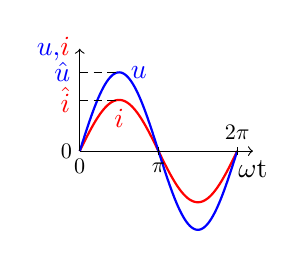
\begin{tikzpicture}
			[
			SinusPlot/.style={domain=0:360, samples=100, variable=\t, thick, color=red},	%Options for sinus plot	
			Achsenpfeil/.style={->},												  		%Style des Achsenpfeils
			HelpLine/.style={densely dashed, very thin}										%Hilfslinien
			]	
			
			%% Definitionen wie Zeigerlänge und Winkel %%  	
			\def\ISpitze{0.65cm};	%Amplitude von I
			\def\USpitze{1cm};		%Amplitude von U
			\def\LenSca{180};		%Die Länge des Sinusplot wird: (max_domain - min_domain) / LenSca; in [cm]
			\def\TickLen{0.05};		% Halbe Länge des Achsen-Tick
			\def\BeschScale{0.8};   %Beschriftungsgrösse Skalierungsfaktor
			
			% Definieren von verschiedenen Koordinaten
			\coordinate (xStart) at (0cm,0cm);		  		  	  %Startpunkt der x-Achse (wt-Achse)
			\coordinate (xEnd)   at (360/\LenSca+0.2,0); 	 	  %Endpunkt der x-Achse (wt-Achse)
			\coordinate (yStart) at (0cm,0cm);    				  %Startpunkt der y-Achse
			\coordinate (yEnd)   at (0cm,\USpitze+0.3cm);	      %Endpunkt der y-Achse 
			
			%%%%%%%%%%%%%%%%%%%%%%%%%% Zeitbereich %%%%%%%%%%%%%%%%%%%%%%%%%%%%%%%
			% Harmonishce Funktionen plotten: 
			\draw[SinusPlot, red]  plot (\t/\LenSca,{\ISpitze*sin(\t)});	%Plot i = I*sin(wt)
			\draw[SinusPlot, blue] plot (\t/\LenSca,{\USpitze*sin(\t)});	%Plot u = U*sin(wt)
			% Achsen Plotten:
			\draw[Achsenpfeil, name path=yAchse] (yStart) -- (yEnd) node[at end, left]{\textcolor{blue}{$u$,}\textcolor{red}{$i$}};	%Plot y-axis
			\draw[Achsenpfeil, name path=xAchse] (xStart) -- (xEnd) node[at end, below]{$\omega$t};  %Plot x-axis
			%Ticks & Beschriftung der x-Achse
			\node[scale = \BeschScale, anchor = north] at (0/\LenSca,0) {$0$};
			\node[scale = \BeschScale, anchor = east]  at (0/\LenSca,0) {$0$};
			\draw (180/\LenSca,\TickLen) -- (180/\LenSca,-\TickLen) node[scale = \BeschScale, below]{$\pi$};		
			\draw (360/\LenSca,-\TickLen) -- (360/\LenSca,\TickLen) node[scale = \BeschScale, above]{$2\pi$};
			% Hilfslinien und Amplitudenbeschriftung
			\draw[HelpLine] (0,\USpitze) -- (90/\LenSca,\USpitze)
				node[at start, left, color=blue]{$\hat{u}$}  	 %Bechriftung der Spannungsamplitude
				node[pos=1.5, color=blue]{$u$};					 %Beschriftung der Spannungsschwingung
			\draw[HelpLine] (0,\ISpitze) -- (90/\LenSca,\ISpitze)
				node[at start, left, color=red]{$\hat{i}$}		 %Bechriftung der Stromamplitude
				node[anchor=west, at end, below, color=red]{$i$};%Beschriftung der Stromschwingung 		
		\end{tikzpicture}
		%-----------------------------------------------------------------------------------------------------------------%	
		
		%-----------------------------------------------------------------------------------------------------------------%	
		\tikzsetnextfilename{WiderstandImWechselstromkreis_c}
		\begin{tikzpicture}	
			[
			Strompfeil/.style={-{Latex[length=2mm]},thick, red},	    %Definiert den Sytle der Strompfeile
			Spannungspfeil/.style={-{Latex[length=2mm]},thick, blue},	%Definiert den Sytle der Spannungsfeile
			]
			
			%% Definitionen wie Zeigerlänge und Winkel - ACHTUNG: Für Länge selbe Werte wie in b) verwenden !! %%  	
			\def\ISpitze{0.65cm};	%Amplitude von I
			\def\USpitze{1cm};		%Amplitude von U
			
			%% Zeigerdiagramm %% 
			\draw[Spannungspfeil] (0,0)      -- ++(0:\USpitze) node[at start, above]{$\hat{\underline{u}}$}; %Spannungspfeil
			\draw[Strompfeil]     (0,-0.1cm) -- ++(0:\ISpitze) node[at start, below] {$\hat{\underline{i}}$};%Strompfeil
		\end{tikzpicture}
		%-----------------------------------------------------------------------------------------------------------------%	
		
	\end{flushright}
	
}\fi

\end{frame}

%%%%%%%%%%%%%%%%%%%%%%%%%%%%%%%%%%%%%%%%%%%%%%%%%%%%%%%%%%%%%%%%%%%%%%%%%%%%%%%%%%%%%%%%%%%%%%%%%%%%%%%%%%%%%%%%%%%%%%

\begin{frame}\frametitle{Induktivität im Wechselstromkreis}

\ifInduktivitaetImWechselstromkreis{
	
	\begin{flushright}
		
		\tikzsetnextfilename{InduktivitaetImWechselstromkreis_b}
		\begin{tikzpicture}
			[
			SinusPlot/.style={domain=0:360, samples=100, variable=\t, thick, color=red},	%Options for sinus plot	
			Achsenpfeil/.style={->},												  		%Style des Achsenpfeils
			HelpLine/.style={densely dashed, very thin},									%Hilfslinien
			Phasenpfeil/.style={-{Latex[length=0.7mm]}, very thin},				  		    %Style des Phasenpfeils (Zeitbereich)
			]	
			
			%% Definitionen wie Zeigerlänge und Winkel %%  	
			\def\ISpitze{0.65cm};	%Amplitude von I
			\def\USpitze{1cm};		%Amplitude von U
			\def\PhiU{90};			%Phasenverschiebung
			\def\LenSca{180};		%Die Länge des Sinusplot wird: (max_domain - min_domain) / LenSca; in [cm]
			\def\TickLen{0.05};		% Halbe Länge des Achsen-Tick
			\def\BeschScale{0.8};   %Beschriftungsgrösse Skalierungsfaktor
			
			% Definieren von verschiedenen Koordinaten
			\coordinate (xStart) at (0cm,0cm);		  		  	  %Startpunkt der x-Achse (wt-Achse)
			\coordinate (xEnd)   at (360/\LenSca+0.2,0); 	 	  %Endpunkt der x-Achse (wt-Achse)
			\coordinate (yStart) at (0cm,0cm);    				  %Startpunkt der y-Achse
			\coordinate (yEnd)   at (0cm,\USpitze+0.3cm);	      %Endpunkt der y-Achse 
			
			%%%%%%%%%%%%%%%%%%%%%%%%%% Zeitbereich %%%%%%%%%%%%%%%%%%%%%%%%%%%%%%%
			% Harmonishce Funktionen plotten: 
			\draw[SinusPlot, red, name path=i]  plot (\t/\LenSca,{\ISpitze*sin(\t)});			%Plot i = I*sin(wt)
			\draw[SinusPlot, blue, name path=u] plot (\t/\LenSca,{\USpitze*sin(\t + \PhiU)});	%Plot u = U*sin(wt + phi)
			% Achsen Plotten:
			\draw[Achsenpfeil, name path=yAchse] (yStart) -- (yEnd) node[at end, left]{\textcolor{blue}{$u$,}\textcolor{red}{$i$}};	%Plot y-axis
			\draw[Achsenpfeil, name path=xAchse] (xStart) -- (xEnd) node[at end, below]{$\omega$t};  %Plot x-axis
			%Ticks & Beschriftung der x-Achse
			\node[scale = \BeschScale, anchor = north] at (0/\LenSca,0) {$0$};
			\node[scale = \BeschScale, anchor = east]  at (0/\LenSca,0) {$0$};
			\draw (180/\LenSca,\TickLen) -- (180/\LenSca,-\TickLen) node[scale = \BeschScale, below]{$\pi$};		
			\draw (360/\LenSca,-\TickLen) -- (360/\LenSca,\TickLen) node[scale = \BeschScale, above]{$2\pi$};
			% Hilfslinien und Amplitudenbeschriftung
			\draw[HelpLine] (0,\USpitze) -- (90/\LenSca - \PhiU/\LenSca,\USpitze)
				node[at start, left, color=blue]{$\hat{u}$}  	 			%Bechriftung der Spannungsamplitude
				node[at end, anchor=west, color=blue]{\hspace{0.1cm}$u$};   %Beschriftung der Spannungsschwingung
			\draw[HelpLine] (0,\ISpitze) -- (90/\LenSca,\ISpitze)
				node[at start, left, color=red]{$\hat{i}$}		 %Bechriftung der Stromamplitude
				node[anchor=west, at end, below, color=red]{$i$};%Beschriftung der Stromschwingung
			% Pfeil der Phasenverschiebung 
			\draw [name intersections={of=i and xAchse, name=interi}, very thin]
				(interi-3) -- ++(-90:\USpitze - 0.1cm) node(HNode1){};	%Plotted Hilfslinie und genereirt Hilfsnode am Ende
			\draw [name intersections={of=u and xAchse, name=interu}, very thin]
				(interu-2) -- ++(-90:\USpitze - 0.1cm) node(HNode2){};	%Plotted Hilfslinie und genereirt Hilfsnode am End	
			\draw[Phasenpfeil] ($(0,0.1cm)+(HNode2)$) -- ($(0,0.1cm)+(HNode1)$)
				node[below, midway]{$\varphi$};									%Plotted Pfeil mit Beschriftung 		
		\end{tikzpicture}
		%-----------------------------------------------------------------------------------------------------------------%	
		
		%-----------------------------------------------------------------------------------------------------------------%	
		\tikzsetnextfilename{InduktivitaetImWechselstromkreis_c}
		\begin{tikzpicture}	
			[
			Strompfeil/.style={-{Latex[length=2mm]},thick, red},	    %Definiert den Sytle der Strompfeile
			Spannungspfeil/.style={-{Latex[length=2mm]},thick, blue},	%Definiert den Sytle der Spannungsfeile
			]
			
			%% Definitionen wie Zeigerlänge und Winkel - ACHTUNG: Für Länge selbe Werte wie in b) verwenden !! %%  	
			\def\ISpitze{0.65cm};	%Amplitude von I
			\def\USpitze{1cm};		%Amplitude von U
			\def\PhiU{90};			%Phasenverschiebung
			
			\coordinate (Ursprung) at (0,0);
			\coordinate (Uend) 	   at (\PhiU:\USpitze);
			\coordinate (Iend) 	   at (0:\ISpitze);
			
			%% Zeigerdiagramm %% 
			\draw[Spannungspfeil] (Ursprung) -- (Uend) node[midway, left]  {$\hat{\underline{u}}$}; %Spannungspfeil
			\draw[Strompfeil]     (Ursprung) -- (Iend) node[midway, below] {$\hat{\underline{i}}$}; %Strompfeil
			%Zwischenwinkel:
			\path (Iend) -- (Ursprung) -- (Uend) 			
				pic[pic text=$\varphi$, draw, -{Latex[length=1mm]}, 
				angle radius = 3mm, angle eccentricity=1.4]
				{angle= Iend--Ursprung--Uend}; % Winkel phi
		\end{tikzpicture}
		%-----------------------------------------------------------------------------------------------------------------%	
		
	\end{flushright}
	
}\fi

\end{frame}

%%%%%%%%%%%%%%%%%%%%%%%%%%%%%%%%%%%%%%%%%%%%%%%%%%%%%%%%%%%%%%%%%%%%%%%%%%%%%%%%%%%%%%%%%%%%%%%%%%%%%%%%%%%%%%%%%%%%%%

\begin{frame}\frametitle{Kondensator im Wechselstromkreis}

\ifKondensatorImWechselstromkreis{
	
	\begin{flushright}
		
		\tikzsetnextfilename{KondensatorImWechselstromkreis_b}
		\begin{tikzpicture}
			[
			SinusPlot/.style={domain=0:360, samples=100, variable=\t, thick, color=red},	%Options for sinus plot	
			Achsenpfeil/.style={->},												  		%Style des Achsenpfeils
			HelpLine/.style={densely dashed, very thin},									%Hilfslinien
			Phasenpfeil/.style={-{Latex[length=0.7mm]}, very thin},				  		    %Style des Phasenpfeils (Zeitbereich)
			]	
			
			%% Definitionen wie Zeigerlänge und Winkel %%  	
			\def\ISpitze{0.65cm};	%Amplitude von I
			\def\USpitze{1cm};		%Amplitude von U
			\def\PhiI{90};			%Phasenverschiebung
			\def\LenSca{180};		%Die Länge des Sinusplot wird: (max_domain - min_domain) / LenSca; in [cm]
			\def\TickLen{0.05};		% Halbe Länge des Achsen-Tick
			\def\BeschScale{0.8};   %Beschriftungsgrösse Skalierungsfaktor
			
			% Definieren von verschiedenen Koordinaten
			\coordinate (xStart) at (0cm,0cm);		  		  	  %Startpunkt der x-Achse (wt-Achse)
			\coordinate (xEnd)   at (360/\LenSca+0.2,0); 	 	  %Endpunkt der x-Achse (wt-Achse)
			\coordinate (yStart) at (0cm,0cm);    				  %Startpunkt der y-Achse
			\coordinate (yEnd)   at (0cm,\USpitze+0.3cm);	      %Endpunkt der y-Achse 
			
			%%%%%%%%%%%%%%%%%%%%%%%%%% Zeitbereich %%%%%%%%%%%%%%%%%%%%%%%%%%%%%%%
			% Harmonishce Funktionen plotten: 
			\draw[SinusPlot, red, name path=i]  plot (\t/\LenSca,{\ISpitze*sin(\t + \PhiI)});%Plot i = I*sin(wt + phi)
			\draw[SinusPlot, blue, name path=u] plot (\t/\LenSca,{\USpitze*sin(\t)});	     %Plot u = U*sin(wt)
			% Achsen Plotten:
			\draw[Achsenpfeil, name path=yAchse] (yStart) -- (yEnd) node[at end, left]{\textcolor{blue}{$u$,}\textcolor{red}{$i$}};	%Plot y-axis
			\draw[Achsenpfeil, name path=xAchse] (xStart) -- (xEnd) node[at end, below]{$\omega$t};  %Plot x-axis
			%Ticks & Beschriftung der x-Achse
			\node[scale = \BeschScale, anchor = north] at (0/\LenSca,0) {$0$};
			\node[scale = \BeschScale, anchor = east]  at (0/\LenSca,0) {$0$};
			\draw (180/\LenSca,\TickLen) -- (180/\LenSca,-\TickLen) node[scale = \BeschScale, anchor=north east]{$\pi$};		
			\draw (360/\LenSca,-\TickLen) -- (360/\LenSca,\TickLen) node[scale = \BeschScale, above]{$2\pi$};
			% Hilfslinien und Amplitudenbeschriftung
			\draw[HelpLine] (0,\USpitze) -- (90/\LenSca,\USpitze)
				node[at start, left, color=blue]{$\hat{u}$}  	 			%Bechriftung der Spannungsamplitude
				node[at end, anchor=west, color=blue]{\hspace{0.1cm}$u$};   %Beschriftung der Spannungsschwingung
			\draw[HelpLine] (0,\ISpitze) -- (90/\LenSca - \PhiI/\LenSca,\ISpitze)
				node[at start, left, color=red]{$\hat{i}$}		 	  %Bechriftung der Stromamplitude
				node[anchor=north west, color=red]{\hspace{0.3cm}$i$};%Beschriftung der Stromschwingung
			% Pfeil der Phasenverschiebung 
			\draw [name intersections={of=i and xAchse, name=interi}, very thin]
				(interi-1) -- ++(-90:\USpitze - 0.1cm) node(HNode1){};	%Plotted Hilfslinie und genereirt Hilfsnode am Ende
			\draw [name intersections={of=u and xAchse, name=interu}, very thin]
				(interu-2) -- ++(-90:\USpitze - 0.1cm) node(HNode2){};	%Plotted Hilfslinie und genereirt Hilfsnode am End	
			\draw[Phasenpfeil] ($(0,0.1cm)+(HNode2)$) -- ($(0,0.1cm)+(HNode1)$)
				node[below, midway]{$\varphi$};									%Plotted Pfeil mit Beschriftung 		
		\end{tikzpicture}
		%-----------------------------------------------------------------------------------------------------------------%	
		
		%-----------------------------------------------------------------------------------------------------------------%	
		\tikzsetnextfilename{KondensatorImWechselstromkreis_c}
		\begin{tikzpicture}	
			[
			Strompfeil/.style={-{Latex[length=2mm]},thick, red},	    %Definiert den Sytle der Strompfeile
			Spannungspfeil/.style={-{Latex[length=2mm]},thick, blue},	%Definiert den Sytle der Spannungsfeile
			]
			
			%% Definitionen wie Zeigerlänge und Winkel - ACHTUNG: Für Länge selbe Werte wie in b) verwenden !! %%  	
			\def\ISpitze{0.65cm};	%Amplitude von I
			\def\USpitze{1cm};		%Amplitude von U
			\def\PhiI{90};			%Phasenverschiebung
			
			\coordinate (Ursprung) at (0,0);
			\coordinate (Uend) 	   at (0:\USpitze);
			\coordinate (Iend) 	   at (\PhiI:\ISpitze);
			
			%% Zeigerdiagramm %% 
			\draw[Spannungspfeil] (Ursprung) -- (Uend) node[midway, below]  {$\hat{\underline{u}}$}; %Spannungspfeil
			\draw[Strompfeil]     (Ursprung) -- (Iend) node[midway, left]   {$\hat{\underline{i}}$}; %Strompfeil
			%Zwischenwinkel:
			\path (Uend) -- (Ursprung) -- (Iend) 			
				pic[pic text=$\varphi$, draw, {Latex[length=1mm]}-, 
				angle radius = 3mm, angle eccentricity=1.4]
				{angle= Uend--Ursprung--Iend}; % Winkel phi
		\end{tikzpicture}
		%-----------------------------------------------------------------------------------------------------------------%	
		
	\end{flushright}
	
}\fi

\end{frame}

%%%%%%%%%%%%%%%%%%%%%%%%%%%%%%%%%%%%%%%%%%%%%%%%%%%%%%%%%%%%%%%%%%%%%%%%%%%%%%%%%%%%%%%%%%%%%%%%%%%%%%%%%%%%%%%%%%%%%%

\begin{frame}\frametitle{Beispiel - Konstruktion eines Zeigerdiagramms}

\ifKonstruktionEinesZeigerdiagramms{
	
	
	\begin{flushright}
		%-----------------------------------------------------------------------------------------------------------------%	
		\tikzsetnextfilename{KonstruktionEinesZeigerdiagramms_b}
		\begin{tikzpicture}	
			[
			Strompfeil/.style={-{Latex[length=2mm]},thick, red},	    			 %Definiert den Sytle der Strompfeile
			Spannungspfeil/.style={-{Latex[length=2mm]},thick, blue},				 %Definiert den Sytle der Spannungsfeile
			HelpNode/.style={at end, inner sep=0pt, outer sep=0pt, minimum size=0pt} %Options für Hilfs-Node am Ende der Hilfslinie
			]
			
			%% Definitionen wie Zeigerlänge und Winkel %%  
			\def\IspitzeE{1.5cm}; %Amplitude von i1
			\def\IspitzeC{1.3cm};	  %Amplitude von ic
			\def\UspitzeE{2.3cm}; %Amplitude von u1
			\def\UspitzeZ{1.1cm}; %Amplitude von uc
			
			\pgfmathsetmacro\PhiD{atan(\IspitzeC/\IspitzeE)}; %Berechne Winkel zwischen i1 und i2
			
			%% Definitionen von verschiedenen Koordinaten %%
			\coordinate (Ursprung) at (0,0);
			\coordinate (UEend)	   at (0:\UspitzeE);
			\coordinate (IEend)	   at (0:\IspitzeE);
			\coordinate (ICend)	   at (90:\IspitzeC);
			\coordinate (UZend)	   at (\PhiD:\UspitzeZ);
			
			%% Zeigerdiagramm %%
			\draw[Spannungspfeil] (Ursprung) -- (UEend) 	node[at end, below]  {$\mzeiger{u}_1$}; %Spannung u1
			\draw[Strompfeil]     (Ursprung) -- (IEend) 	node[near end, below]{$\mzeiger{i}_1$}; %Strom i1
			\draw[Strompfeil]     (IEend)  -- ++(ICend) 	node[near end, right]{$\mzeiger{i}_C$} node[HelpNode](NodeICend){}; %Strom iC
			\draw[Strompfeil]     (Ursprung) -- (NodeICend) node[near end, above]{$\mzeiger{i}_2$}; %Strom i2
			\draw[Spannungspfeil] (Ursprung) -- (UZend) 	node[midway, above]  {$\mzeiger{u}_2$}; %Spannung u2
			\draw[Spannungspfeil] (UEend)  -- ++(UZend) 	node[near end, below]{$\mzeiger{u}_2$} node[HelpNode](NodeUZend){}; %Spannung u2
			\draw[Spannungspfeil, color=black] (Ursprung) -- (NodeUZend) node[near end, above]{$\mzeiger{u}$}; %Quellspannung
			
			% Winkelbeschriftungen %
			\path (UEend) -- (Ursprung) -- (NodeUZend) 			
				pic[pic text=$\varphi_1$, draw, -{Latex[length=1mm]}, 
				angle radius = 17mm, angle eccentricity=1.13]
				{angle= UEend--Ursprung--NodeUZend}; % Winkel phi1
			\path (NodeUZend) -- (Ursprung) -- (NodeICend) 			
				pic[pic text=$\varphi_2$, draw, -{Latex[length=1mm]}, 
				angle radius = 6.5mm, angle eccentricity=1.3]
				{angle= NodeUZend--Ursprung--NodeICend}; % Winkel phi2	
		\end{tikzpicture}
		%-----------------------------------------------------------------------------------------------------------------%		 	
	\end{flushright}

}\fi

\end{frame}

%%%%%%%%%%%%%%%%%%%%%%%%%%%%%%%%%%%%%%%%%%%%%%%%%%%%%%%%%%%%%%%%%%%%%%%%%%%%%%%%%%%%%%%%%%%%%%%%%%%%%%%%%%%%%%%%%%%%%%

\begin{frame}\frametitle{Grundbegriffe der komplexen Rechnung}

\ifGrundbegriffeDerKomplexenRechnung{
		
	\begin{flushright}
		%-----------------------------------------------------------------------------------------------------------------%
		\tikzsetnextfilename{GrundbegriffeDerKomplexenRechnung_a}
		\begin{tikzpicture}
			%Verschiedene Styles definieren:
			[
			 Achsenpfeil/.style={->},												  %Style des Achsenpfeils
		     HelpNode/.style={at end, inner sep=0pt, outer sep=0pt, minimum size=0pt},%Options für Hilfs-Node (z.B. am Ende eines Zeigers)
			 Zeiger/.style={-{Latex[length=2mm]}, thick, blue},					      %Style der komplexen Zeiger
		     Winkelpfeil/.style={draw, -{Latex[length=1mm]}, angle radius = 9mm},	  %Style der Winkelpfeil 
		     HelpLine/.style={densely dashed, very thin},							  %Hilfslinien 								  
			]
			% Verschiedene Variabeln definieren:
			\def\Zlen{1.5cm}; 	%Länge des komplexen Zeigers
			\def\Zphi{45};		%Winkel des komplexen Zeigers
			
			% Definieren von verschiedenen Koordinaten
			\coordinate (xStart)   at (-0.6cm,0);		   %Startpunkt der x-Achse (wt-Achse)
			\coordinate (xEnd) 	   at (\Zlen+0.8cm,0); 	   %Endpunkt der x-Achse (wt-Achse)
			\coordinate (yStart)   at (0cm,-\Zlen);  %Startpunkt der y-Achse
			\coordinate (yEnd) 	   at (0cm,\Zlen+0.2cm);   %Endpunkt der y-Achse 
			\coordinate (Ursprung) at (0,0);
		
			%%%%%%%%%%%%%%%%%%%%%%%%%% Zeigerdiagramm %%%%%%%%%%%%%%%%%%%%%%%%%%%%%%%%%%%
			% Graue Box
			\fill[gray!25] (-1.3,-1.7) --++ (3.9,0) --++ (0,3.7) --++ (-3.9,0) -- cycle;
			% Plotten der Achsen
			\draw[Achsenpfeil, name path=xAchse] (xStart) -- (xEnd) node[below]{$X$};  	%Plot x-axis
			\draw[Achsenpfeil, name path=yAchse] (yStart) -- (yEnd) node[left] {$jY$}; 	%Plot y-axis
			\node[anchor=north east] at (Ursprung) {$0$}; 								%Beschriftnug des Urpsrungs 
			% Plotten der Zeiger 
			\draw[Zeiger] (Ursprung) --++ (\Zphi:\Zlen)
				node[near end, left] {$\lvert\underline{Z}\rvert\textcolor{black}{=Z}$}
				node(tmp1) [HelpNode]{}; %Komplexer Zeiger nach oben
			\draw[Zeiger] (Ursprung) --++ (-\Zphi:\Zlen)
				node[midway, left, black, anchor=north east] {$Z$}
				node(tmp2) [HelpNode]{}; %Komplexer Zeiger nach unten
			% Winkel-Beschriftung
			\path (tmp2) -- (Ursprung) -- (xEnd) 
				pic[Winkelpfeil, pic text=$\varphi$ ] {angle = xEnd--Ursprung--tmp1};%Winkelpfiel
			\path (xEnd) -- (Ursprung) -- (tmp1) 
				pic[Winkelpfeil, pic text=-$\varphi$, {Latex[length=1mm]}-] {angle = tmp2--Ursprung--xEnd};%Winkelpfie	
			% Hilfslinien
			\draw[HelpLine] (Ursprung |- tmp1) -- (tmp1) node[at start, anchor=east, scale=0.8] {$Y=\operatorname{Im}\{\underline{Z}\}$};
			\draw[HelpLine] (Ursprung |- tmp2) -- (tmp2) node[at start, anchor=east, scale=0.8] {$Y=-\operatorname{Im}\{\underline{Z}\}$};	
			\draw[HelpLine] (tmp1) 			   -- (tmp2) node[midway, anchor=south west, scale=0.8] {$X=\operatorname{Re}\{\underline{Z}\}$};
			% Beschriftungen
			\node[anchor=south west, scale=0.8, draw] (Algebra)  at (tmp1) {$\textcolor{blue}{\underline{Z}}=X+jY$};
			\node[anchor=north west, scale=0.8, draw] 			 at (tmp2) {$\textcolor{blue}{\underline{Z}^*}=X-jY$};
			\node[above = 0.8cm of Algebra, align=left]    (AlgebraText) {Algebraische\\ Darstellung}; 			  %Beschrifuntg Algebra
			\node[left = 0.6cm of AlgebraText, align=left] (EbeneText)   {Komplexe\\ (Gauss'sche)\\ Zahlenebene}; %Beschrigtung Gauss
			\draw (Algebra) 		-- (AlgebraText);	%Strich für Algebraische Darstellung
			\draw (EbeneText.south) --++(230:0.4);		%Strich für Gauss-Ebene	
		\end{tikzpicture}
		%------------------------------------------------------------------------------	-----------------------------------%	

	\end{flushright}
	
}\fi

\end{frame}

%%%%%%%%%%%%%%%%%%%%%%%%%%%%%%%%%%%%%%%%%%%%%%%%%%%%%%%%%%%%%%%%%%%%%%%%%%%%%%%%%%%%%%%%%%%%%%%%%%%%%%%%%%%%%%%%%%%%%%

\begin{frame}\frametitle{Rechenoperationen mit komplexen Zahlen}

\ifRechenOperationenMitKomplexenZahlen{
	
	\begin{flushright}
		%-----------------------------------------------------------------------------------------------------------------%
		\tikzsetnextfilename{RechenOperationenMitKomplexenZahlen_a}
		\begin{tikzpicture}
			%Verschiedene Styles definieren:
			[
			 Achsenpfeil/.style={->},												  %Style des Achsenpfeils
			 HelpNode/.style={at end, inner sep=0pt, outer sep=0pt, minimum size=0pt},%Options für Hilfs-Node (z.B. am Ende eines Zeigers)
			 Zeiger/.style={-{Latex[length=2mm]}, thick},					          %Style der komplexen Zeiger
			 Winkelpfeil/.style={draw, -{Latex[length=1mm]}, angle radius = 9mm},	  %Style der Winkelpfeil 								  
			]
			% Verschiedene Variabeln definieren:
			\def\Zeins{1.5cm}; 	  %Länge von Z1
			\def\Zzwei{0.5cm};	  %Länge von Z2
			\def\PhiE{30};		  %Winkel Phi1 von Z1
			\def\PhiZ{150};		  %Winkel Phi2 von Z2
			\def\BeschScale{0.8}; %Skalierungsfaktor für Beschriftung
			
			% Definieren von verschiedenen Koordinaten
			\coordinate (xStart)   at (-0.5cm,0);		   %Startpunkt der x-Achse (wt-Achse)
			\coordinate (xEnd) 	   at (2cm,0);   %Endpunkt der x-Achse (wt-Achse)
			\coordinate (yStart)   at (0cm,-0.1cm);  	   %Startpunkt der y-Achse
			\coordinate (yEnd) 	   at (0cm,1.3cm); 	   %Endpunkt der y-Achse 
			\coordinate (Ursprung) at (0,0);
			
			%%%%%%%%%%%%%%%%%%%%%%%%%% Zeigerdiagramm %%%%%%%%%%%%%%%%%%%%%%%%%%%%%%%%%%%
			% Plotten der Achsen
			\draw[Achsenpfeil, name path=xAchse] (xStart) -- (xEnd) node[below]{$X$};  	%Plot x-axis
			\draw[Achsenpfeil, name path=yAchse] (yStart) -- (yEnd) node[left] {$jY$}; 	%Plot y-axis
			\node[anchor=north east] at (Ursprung) {$0$}; 								%Beschriftnug des Urpsrungs 
			% Plotten der Zeiger 
			\draw[Zeiger] (Ursprung) --++ (\PhiE:\Zeins)
				node[pos=0.65, above, scale=\BeschScale] {$\underline{Z}_1$}
				node(tmp1) [HelpNode]{}; %Komplexer Zeiger Z1
			\draw[Zeiger] (Ursprung) --++ (\PhiZ:\Zzwei)
				node[near end, above, scale=\BeschScale] {$\underline{Z}_2$}
				node(tmp2) [HelpNode]{}; %Komplexer Zeiger Z2
			\draw[Zeiger, blue, densely dashed] (tmp1) --++ (\PhiZ+180:\Zzwei)
				node[near end, above, anchor= south west, scale=\BeschScale] {-$\underline{Z}_2$}
				node(tmp3) [HelpNode]{}; % -Z2 an Z1
			\draw[Zeiger, blue, densely dashed] (tmp1) --++ (\PhiZ:\Zzwei)
				node[midway, above, anchor=south west, scale=\BeschScale] {$\underline{Z}_2$}
				node(tmp4) [HelpNode]{}; % +Z2 an Z1
			\draw[Zeiger, blue] (Ursprung) --++ (tmp3)
				node[near end, right, anchor=north west, scale=\BeschScale] {$\underline{Z}_1-\underline{Z}_2$}; % Z1 - Z2
			\draw[Zeiger, blue] (Ursprung) --++ (tmp4)
				node[pos=0.9, left, anchor=south east, scale=\BeschScale] {$\underline{Z}_1+\underline{Z}_2$}; % Z1 + Z2
			% Beschriftung
			\node[anchor=north west, align=left, scale=\BeschScale] at (xEnd |- yEnd)
				{$\underline{Z}_1=X_1+jY_1$\\ $\underline{Z}_2=X_2+jY_2$};
		\end{tikzpicture}
		%------------------------------------------------------------------------------	-----------------------------------%
			
		%------------------------------------------------------------------------------------------------------------------%
		\tikzsetnextfilename{RechenOperationenMitKomplexenZahlen_b}
		\begin{tikzpicture}
			%Verschiedene Styles definieren:
			[
			 Achsenpfeil/.style={->},												  %Style des Achsenpfeils
			 HelpNode/.style={at end, inner sep=0pt, outer sep=0pt, minimum size=0pt},%Options für Hilfs-Node (z.B. am Ende eines Zeigers)
			 Zeiger/.style={-{Latex[length=2mm]}, thick},					          %Style der komplexen Zeiger
			 Winkelpfeil/.style={draw, -{Latex[length=1mm]}},	  					  %Style der Winkelpfeil 								  
			]
			% Verschiedene Variabeln definieren:
			\def\Zeins{1.2}; 	  %Länge von Z1 [cm]
			\def\Zzwei{1};	      %Länge von Z2 [cm]
			\def\PhiE{30};		  %Winkel Phi1 von Z1 [°]
			\def\PhiZ{100};		  %Winkel Phi2 von Z2 [°]
			\def\BeschScale{0.8}; %Skalierungsfaktor für Beschriftung
			
			% Definieren von verschiedenen Koordinaten
			\coordinate (xStart)   at (-0.5cm,0);   %Startpunkt der x-Achse (wt-Achse)
			\coordinate (xEnd) 	   at (2cm,0);      %Endpunkt der x-Achse (wt-Achse)
			\coordinate (yStart)   at (0cm,-0.1cm); %Startpunkt der y-Achse
			\coordinate (yEnd) 	   at (0cm,1.2cm); 	%Endpunkt der y-Achse 
			\coordinate (Ursprung) at (0,0);
			
			%%%%%%%%%%%%%%%%%%%%%%%%%% Zeigerdiagramm %%%%%%%%%%%%%%%%%%%%%%%%%%%%%%%%%%%
			% Plotten der Achsen
			\draw[Achsenpfeil, name path=xAchse] (xStart) -- (xEnd) node[below]{$X$};  	%Plot x-axis
			\draw[Achsenpfeil, name path=yAchse] (yStart) -- (yEnd) node[left] {$jY$}; 	%Plot y-axis
			\node[anchor=north east] at (Ursprung) {$0$}; 								%Beschriftnug des Urpsrungs 
			% Plotten der Zeiger 
			\draw[Zeiger] (Ursprung) --++ (\PhiE:\Zeins)
				node[at end, right, scale=\BeschScale] {$\underline{Z}_1$}
				node(tmp1) [HelpNode]{}; % Zeiger Z1
			\draw[Zeiger] (Ursprung) --++ (\PhiZ:\Zzwei)
				node[near end, left, scale=\BeschScale] {$\underline{Z}_2$}
				node(tmp2) [HelpNode]{};  % Zeiger Z2
			\draw[Zeiger, blue] (Ursprung) --++ (\PhiE+\PhiZ:\Zeins*\Zzwei)
				node[at end, above, scale=\BeschScale] {$\underline{Z}_1\underline{Z}_2$}
				node(tmp3) [HelpNode]{}; % Z1*Z2
			% Winkel-Beschriftung
			\path (xEnd) -- (Ursprung) -- (tmp1)
				pic[Winkelpfeil, pic text options={scale=\BeschScale}, pic text=$\varphi_1$, -{Latex[length=1mm]}, angle radius = 7mm, angle eccentricity=1.2]
				{angle = xEnd--Ursprung--tmp1}; %phi1
			\path (xEnd) -- (Ursprung) -- (tmp2)
				pic[Winkelpfeil, pic text options={scale=\BeschScale}, pic text=$\varphi_2$, -{Latex[length=1mm]}, angle radius = 5mm, angle eccentricity=1.3]
				{angle = xEnd--Ursprung--tmp2}; %phi2
			\path (xEnd) -- (Ursprung) -- (tmp3)
				pic[Winkelpfeil, -{Latex[length=1mm]}, angle radius = 3mm, blue]
				{angle = xEnd--Ursprung--tmp3}; %phi3 = phi1 + phi2	
			\node[anchor=south east, blue, scale=\BeschScale] (phi3) at (-0.1,0) {$\varphi_1+\varphi_2$};
			% Beschriftung
			\node[anchor=north west, align=left, scale=\BeschScale] at (xEnd |- yEnd)
				{$\underline{Z}_1=Z_1\mathrm{e}^{\mathrm{j}\varphi_1}$\\ $\underline{Z}_2=Z_2\mathrm{e}^{\mathrm{j}\varphi_2}$};	
		\end{tikzpicture}
		%------------------------------------------------------------------------------	-----------------------------------%
		
		%------------------------------------------------------------------------------------------------------------------%
		\tikzsetnextfilename{RechenOperationenMitKomplexenZahlen_c}
		\begin{tikzpicture}
			%Verschiedene Styles definieren:
			[
			 Achsenpfeil/.style={->},												  %Style des Achsenpfeils
			 HelpNode/.style={at end, inner sep=0pt, outer sep=0pt, minimum size=0pt},%Options für Hilfs-Node (z.B. am Ende eines Zeigers)
			 Zeiger/.style={-{Latex[length=2mm]}, thick},					          %Style der komplexen Zeiger
			 Winkelpfeil/.style={draw, -{Latex[length=1mm]}},	  					  %Style der Winkelpfeil 								  
			]
			% Verschiedene Variabeln definieren: ACHTUNG: Länge/Winkel von Z1 hängen von den Werten aus b) ab!!!
			\def\Zeins{1.2*1};    %Länge von Z1 [cm]
			\def\Zzwei{1};	      %Länge von Z2 [cm]
			\def\PhiE{130};		  %Winkel Phi1 von Z1 [°]
			\def\PhiZ{100};		  %Winkel Phi2 von Z2 [°]
			\def\BeschScale{0.8}; %Skalierungsfaktor für Beschriftung
			
			% Definieren von verschiedenen Koordinaten
			\coordinate (xStart)   at (-0.5cm,0);   %Startpunkt der x-Achse (wt-Achse)
			\coordinate (xEnd) 	   at (2cm,0);      %Endpunkt der x-Achse (wt-Achse)
			\coordinate (yStart)   at (0cm,-0.1cm); %Startpunkt der y-Achse
			\coordinate (yEnd) 	   at (0cm,1.2cm); 	%Endpunkt der y-Achse 
			\coordinate (Ursprung) at (0,0);
			
			%%%%%%%%%%%%%%%%%%%%%%%%%% Zeigerdiagramm %%%%%%%%%%%%%%%%%%%%%%%%%%%%%%%%%%%
			% Plotten der Achsen
			\draw[Achsenpfeil, name path=xAchse] (xStart) -- (xEnd) node[below]{$X$};  	%Plot x-axis
			\draw[Achsenpfeil, name path=yAchse] (yStart) -- (yEnd) node[left] {$jY$}; 	%Plot y-axis
			\node[anchor=north east] at (Ursprung) {$0$}; 								%Beschriftnug des Urpsrungs 
			% Plotten der Zeiger 
			\draw[Zeiger] (Ursprung) --++ (\PhiE:\Zeins)
				node[at end, above, scale=\BeschScale] {$\underline{Z}_1$}
				node(tmp1) [HelpNode]{}; % Zeiger Z1
			\draw[Zeiger] (Ursprung) --++ (\PhiZ:\Zzwei)
				node[near end, left, scale=\BeschScale] {$\underline{Z}_2$}
				node(tmp2) [HelpNode]{};  % Zeiger Z2
			\draw[Zeiger, blue] (Ursprung) --++ (\PhiE-\PhiZ:\Zeins/\Zzwei)
				node[at end, above, scale=\BeschScale] {$\underline{Z}_1/\underline{Z}_2$}
				node(tmp3) [HelpNode]{}; % Z1*Z2
			% Winkel-Beschriftung
			\path (xEnd) -- (Ursprung) -- (tmp1)
				pic[Winkelpfeil, -{Latex[length=1mm]}, angle radius = 3mm]
				{angle = xEnd--Ursprung--tmp1}; %phi1
			\node[anchor=south east, scale=\BeschScale] (phi1) at (-0.1,0) {$\varphi_1$}; %Beschriftung Phi1
			\path (xEnd) -- (Ursprung) -- (tmp2)
				pic[Winkelpfeil, pic text options={scale=\BeschScale}, pic text=$\varphi_2$, -{Latex[length=1mm]}, angle radius = 5mm, angle eccentricity=1.3]
				{angle = xEnd--Ursprung--tmp2}; %phi2
			\path (xEnd) -- (Ursprung) -- (tmp3)
				pic[Winkelpfeil, pic text options={scale=\BeschScale}, pic text=$\varphi_1-\varphi_2$, -{Latex[length=1mm]}, angle radius = 3mm, blue, angle radius = 7mm, angle eccentricity=1, anchor=west]
				{angle = xEnd--Ursprung--tmp3}; %phi3 = phi1 + phi2	
			% Beschriftung
			\node[anchor=north west, align=left, scale=\BeschScale] at (xEnd |- yEnd)
				{$\underline{Z}_1=Z_1\mathrm{e}^{\mathrm{j}\varphi_1}$\\ $\underline{Z}_2=Z_2\mathrm{e}^{\mathrm{j}\varphi_2}$};	
		\end{tikzpicture}
		%------------------------------------------------------------------------------	-----------------------------------%
		
		%------------------------------------------------------------------------------------------------------------------%
		\tikzsetnextfilename{RechenOperationenMitKomplexenZahlen_d}
		\begin{tikzpicture}
			%Verschiedene Styles definieren:
			[
			 Achsenpfeil/.style={->},												  %Style des Achsenpfeils
			 HelpNode/.style={at end, inner sep=0pt, outer sep=0pt, minimum size=0pt},%Options für Hilfs-Node (z.B. am Ende eines Zeigers)
			 Zeiger/.style={-{Latex[length=2mm]}, thick},					          %Style der komplexen Zeiger							  
			]
			% Verschiedene Variabeln definieren:
			\def\Zeins{0.8};  	  %Länge von Z1 [cm]
			\def\PhiE{40};		  %Winkel Phi1 von Z1 [°]
			\def\BeschScale{0.8}; %Skalierungsfaktor für Beschriftung
			\def\Xoff{-2};		  %X-Achsen Offset zwischen links & rechts
			
			% Definieren von verschiedenen Koordinaten
			\coordinate (xStart)    at (-0.5cm,0);   %Startpunkt der x-Achse (wt-Achse)
			\coordinate (xEnd) 	    at (1.2cm,0);    %Endpunkt der x-Achse (wt-Achse)
			\coordinate (yStart)    at (0cm,-0.1cm); %Startpunkt der y-Achse
			\coordinate (yEnd) 	    at (0cm,0.8cm);  %Endpunkt der y-Achse 
			\coordinate (Ursprung)  at (0,0);			
			%%%%%%%%%%%%%%%%%%%%%%%%%% Zeigerdiagramm rechts %%%%%%%%%%%%%%%%%%%%%%%%%%%%%%%%%%%
			% Plotten der Achsen
			\draw[Achsenpfeil, name path=xAchse] (xStart) -- (xEnd) node[below]{$X$};  	%Plot x-axis
			\draw[Achsenpfeil, name path=yAchse] (yStart) -- (yEnd) node[left] {$jY$}; 	%Plot y-axis
			\node[anchor=north east] at (Ursprung) {$0$}; 								%Beschriftnug des Urpsrungs 
			% Plotten der Zeiger 
			\draw[Zeiger] (Ursprung) --++ (\PhiE:\Zeins)
				node[at end, above, scale=\BeschScale] {$\underline{Z}$}
				node(tmp1) [HelpNode]{}; % Zeiger Z1
			\draw[Zeiger, blue] (Ursprung) --++ (\PhiE-90:\Zeins)
				node[at end, right, scale=\BeschScale] {-$j\underline{Z}$}
				node(tmp2) [HelpNode]{}; % Zeiger -j*Z1
			% Winkelbeschrifutng
			\path (tmp2) -- (Ursprung) -- (tmp1)
				pic[draw, pic text options={scale=\BeschScale, anchor=north west}, pic text=-$\frac{\pi}{2}$, {Latex[length=1mm]}-,
				angle radius = 3mm, angle eccentricity=0.9]
				{angle = tmp2--Ursprung--tmp1}; %-pi/2
			%%%%%%%%%%%%%%%%%%%%%%%%%% Zeigerdiagramm links %%%%%%%%%%%%%%%%%%%%%%%%%%%%%%%%%%%
			\begin{scope}[xshift=-2cm]
				%Koordinaten müssen nochmals definiert werden, sonst werden sie nicht geshifted... 
				\coordinate (xStart)    at (-0.5cm,0);   %Startpunkt der x-Achse (wt-Achse)
				\coordinate (xEnd) 	    at (1.2cm,0);    %Endpunkt der x-Achse (wt-Achse)
				\coordinate (yStart)    at (0cm,-0.1cm); %Startpunkt der y-Achse
				\coordinate (yEnd) 	    at (0cm,0.8cm);  %Endpunkt der y-Achse 
				\coordinate (Ursprung)  at (0,0);
				% Plotten der Achsen
				\draw[Achsenpfeil, name path=xAchse] (xStart) -- (xEnd) node[below]{$X$};  	%Plot x-axis
				\draw[Achsenpfeil, name path=yAchse] (yStart) -- (yEnd) node[left] {$jY$}; 	%Plot y-axis
				\node[anchor=north east] at (Ursprung) {$0$}; 								%Beschriftnug des Urpsrungs 
				% Plotten der Zeiger 
				\draw[Zeiger] (Ursprung) --++ (\PhiE:\Zeins)
					node[at end, above, scale=\BeschScale] {$\underline{Z}$}
					node(tmp1) [HelpNode]{}; % Zeiger Z1
				\draw[Zeiger, blue] (Ursprung) --++ (\PhiE+90:\Zeins)
					node[at end, left, scale=\BeschScale] {$j\underline{Z}$}
					node(tmp2) [HelpNode]{}; % Zeiger j*Z1
				% Winkelbeschrifutng
				\path (tmp1) -- (Ursprung) -- (tmp2)
					pic[draw, pic text options={scale=\BeschScale, anchor=south west}, pic text=$\frac{\pi}{2}$, -{Latex[length=1mm]},
					angle radius = 3mm, angle eccentricity=0.85]
					{angle = tmp1--Ursprung--tmp2}; %pi/2	
			\end{scope}	
		\end{tikzpicture}
		%------------------------------------------------------------------------------	-----------------------------------%
			
	\end{flushright}	
}\fi
\end{frame}

%%%%%%%%%%%%%%%%%%%%%%%%%%%%%%%%%%%%%%%%%%%%%%%%%%%%%%%%%%%%%%%%%%%%%%%%%%%%%%%%%%%%%%%%%%%%%%%%%%%%%%%%%%%%%%%%%%%%%%

\begin{frame}\frametitle{Komplexe Wechselstromrechnung}

\ifKomplexeWechselstromrechnung{	
	\begin{flushright}
		%------------------------------------------------------------------------------------------------------------------%
		\tikzsetnextfilename{KomplexeWechselstromrechnung_a}
		\begin{tikzpicture}
			%Verschiedene Styles definieren:
			[
			 Achsenpfeil/.style={->},												  %Style des Achsenpfeils
			 HelpNode/.style={at end, inner sep=0pt, outer sep=0pt, minimum size=0pt},%Options für Hilfs-Node (z.B. am Ende eines Zeigers)
			 Zeiger/.style={-{Latex[length=2mm]}, thick, blue},					      %Style der komplexen Zeiger
			 Winkelpfeil/.style={draw, -{Latex[length=1mm]}},	  					  %Style der Winkelpfeil 
			 HelpLine/.style={densely dashed, very thin},							  %Hilfslinien 								  
			]
			% Verschiedene Variabeln definieren: ACHTUNG: Länge/Winkel von Z1 hängen von den Werten aus b) ab!!!
			\def\USpitze{1.9};    %Betrag von u [cm]
			\def\PhiU{20};		  %Initalwinkel für t=0 [°]
			\def\Phiwt{40};	  %Winkel nach Zeit t [°]
			
			% Definieren von verschiedenen Koordinaten
			\coordinate (xStart)   at (-0.1cm,0);   %Startpunkt der x-Achse (wt-Achse)
			\coordinate (xEnd) 	   at (2cm,0);      %Endpunkt der x-Achse (wt-Achse)
			\coordinate (yStart)   at (0cm,-0.1cm); %Startpunkt der y-Achse
			\coordinate (yEnd) 	   at (0cm,2.5cm); 	%Endpunkt der y-Achse 
			\coordinate (Ursprung) at (0,0);
			
			%%%%%%%%%%%%%%%%%%%%%%%%%% Zeigerdiagramm %%%%%%%%%%%%%%%%%%%%%%%%%%%%%%%%%%%
			% Plotten der Achsen
			\draw[Achsenpfeil, name path=xAchse] (xStart) -- (xEnd) node[below]{$\operatorname{Re}(\underline{u})$};  	%Plot x-axis
			\draw[Achsenpfeil, name path=yAchse] (yStart) -- (yEnd) node[right] {$j\operatorname{Im}(\underline{u})$}; 	%Plot y-axis 
			% Plotten der Zeiger 
			\draw[Zeiger, densely dashed] (Ursprung) --++ (\PhiU:\USpitze)
				node[near end, below] {$\underline{\hat{u}}$}
				node[at end, anchor=west, black] {$\hat{u}e^{j\varphi_u}$}
				node(uEnd1) [HelpNode]{}; % Zeiger Z1
			\draw[Zeiger] (Ursprung) --++ (\PhiU+\Phiwt:\USpitze)
				node[near end, left] {$\underline{\hat{u}}'$}
				node(uEnd2) [HelpNode]{};  % Zeiger Z2
			% Winkel-Beschriftung
			\path (xEnd) -- (Ursprung) -- (uEnd1)
				pic[Winkelpfeil, pic text options={anchor=west}, pic text=$\varphi_u$, -{Latex[length=1mm]}, angle radius = 9mm]
				{angle = xEnd--Ursprung--uEnd1}; %phiu
			\path (uEnd1) -- (Ursprung) -- (uEnd2)
				pic[Winkelpfeil, pic text options={}, pic text=$\omega t$, -{Latex[length=1mm]}, angle radius = 10mm, 
				angle eccentricity=0.8]
				{angle = uEnd1--Ursprung--uEnd2}; %wt
			% Hilfslinien
			\draw[HelpLine]  (uEnd2) -- (uEnd2 |- Ursprung) node[near start, anchor=west](BeschImag){$j\hat{u}\sin(\omega t + \varphi_u)$};
			\draw[HelpLine]  (uEnd2) -- (uEnd2 -| Ursprung);
			% Pfeil für Drechrichtung 
			\draw[Zeiger, red] (50:\USpitze+0.1) 
				arc[start angle=50, delta angle=20, x radius=\USpitze+0.05, y radius=\USpitze+0.05]
				node[near end, anchor=south, black] (BeschReal) {$\hat{u}\cos(\omega t + \varphi_u)$} %Beschriftung des Realteils
				node[midway, right]{$\omega$};
			%Striche für Beschriftung
			\draw ($(BeschReal.south) + (-0.4,0.1)$) --++(-90:0.25);
			\draw ($(BeschImag.south) + (-0.5,0.1)$) --++(220:0.35);	
		\end{tikzpicture}
		%------------------------------------------------------------------------------	-----------------------------------%	
	\end{flushright}	
}\fi
\end{frame}

%%%%%%%%%%%%%%%%%%%%%%%%%%%%%%%%%%%%%%%%%%%%%%%%%%%%%%%%%%%%%%%%%%%%%%%%%%%%%%%%%%%%%%%%%%%%%%%%%%%%%%%%%%%%%%%%%%%%%%

\begin{frame}\frametitle{Zeiger für komplexe Wechselstromrechnung}

\ifZeigerFuerKomplexeWechselstromrechnung{	
	\begin{flushright}
		%------------------------------------------------------------------------------------------------------------------%
		\tikzsetnextfilename{ZeigerFuerKomplexeWechselstromrechnung_a}
		\begin{tikzpicture}
			[
			Spannungspfeil/.style={-{Latex[length=2mm]},thick, blue},						%Definiert den Sytle der Strompfeile
			SinusPlot/.style={domain=0:360, samples=100, variable=\t, thick, color=blue},	%Options for sinus plot	
			Achsenpfeil/.style={->},												  		%Style des Achsenpfeils
			HelpNode/.style={at end, inner sep=0pt, outer sep=0pt, minimum size=0pt},		%Options für Hilfs-Node am Ende der Hilfslinie
			Winkelpfeil/.style={draw, -{Latex[length=1mm]}},								%Style der  Winkelpfeile
			HelpLine/.style={densely dashed, very thin}										%Hilfslinien
			]	
			
			%% Definitionen wie Zeigerlänge etc.. %% 
			\def\USpitze{0.8cm};		%Amplitude von U
			\def\LenSca{200};			%Die Länge des Sinusplot wird: (max_domain - min_domain) / LenSca; in [cm]
			\def\PhiO{0};				%Winkel wt0
			\def\PhiE{30};				%Winkel wt1			
			\def\PhiZ{60};				%Winkel wt2
			\def\TickLen{0.05}			% Halbe Länge des Achsen-Tick
			\def\BeschScale{0.8}		%Skalireung der Achsenbeschrifung
			
			% Definieren von verschiedenen Koordinaten
			\coordinate (xStart) at (-0.2cm,0);		  		  %Startpunkt der x-Achse (wt-Achse)
			\coordinate (xEnd) at (360cm/\LenSca+0.2cm,0); 	  %Endpunkt der x-Achse (wt-Achse)
			\coordinate (yStart) at (0cm,-0.2cm);   		  %Startpunkt der y-Achse
			\coordinate (yEnd) at (0cm,\USpitze+0.2cm);	      %Endpunkt der y-Achse 
			
			%%%%%%%%%%%%%%%%%%%%%%%%%% Zeitbereich %%%%%%%%%%%%%%%%%%%%%%%%%%%%%%%
			% Harmonishce Funktionen plotten: 
			\draw[SinusPlot, name path=u] plot (\t/\LenSca,{\USpitze*sin(\t+\PhiO)});		%Plot u = U*sin(wt+phi0)
			% Achsen Plotten:
			\draw[Achsenpfeil, name path=yAchse] (yStart) -- (yEnd) node[at end, right]{$u$};		 %Plot y-axis
			\draw[Achsenpfeil, name path=xAchse] (xStart) -- (xEnd) node[at end, below]{$\omega$t};  %Plot x-axis
			%Ticks & Beschriftung der x-Achse
			\node[scale = \BeschScale, anchor = north east] at (0/\LenSca,0) {$0$};
			\draw (90/\LenSca,\TickLen) -- (90/\LenSca,-\TickLen) node[scale = \BeschScale, below]{$\frac{\pi}{2}$};		
			\draw (180/\LenSca,\TickLen) -- (180/\LenSca,-\TickLen) node[scale = \BeschScale, below]{$\pi$};
			\draw (270/\LenSca,-\TickLen) -- (270/\LenSca,\TickLen) node[scale = \BeschScale, above]{$\frac{3\pi}{2}$};
			\draw (360/\LenSca,-\TickLen) -- (360/\LenSca,\TickLen) node[scale = \BeschScale, above]{$2\pi$};
			% Bechriftung der Spannungsamplitude:
			\draw[HelpLine] (0,\USpitze) -- (90/\LenSca-\PhiO/\LenSca,\USpitze)
				node[at start, left, color=blue]{$\hat{u}$};
			
			%%%%%%%%%%%%%%%%%%%%%%%%%% Zeigerdiagramm %%%%%%%%%%%%%%%%%%%%%%%%%%%%%%%%%%%
			% Kreise 
			\coordinate (Ursprung) at ($(0,0) - (\USpitze+0.5cm,0)$); 	%Definiert den Ursprung des Zeigerdiagramms
			\draw (Ursprung) circle  (\USpitze);						%Kreis mit Radius von U
			\node[anchor = north east] at (Ursprung) {M};				%Beschriftung des Mittelpunktes
			% Achsen
			\draw[->] ($(Ursprung) - (0,\USpitze+0.2cm)$) -- ($(Ursprung) + (0,\USpitze+0.2cm)$) %Zeichnet y-achse
				node[at start, left, scale = \BeschScale]{$\frac{3\pi}{2}$}					 % 3Pi/2 Beschr.
				node[at end, left, scale = \BeschScale]{{$\frac{\pi}{2}$}}					 % Pi/2 Beschr.
				node[at end, right, scale= \BeschScale]{\textcolor{gray}{\hspace{1mm}jy}};	 % jy Beschr.
			\draw[->] ($(Ursprung) - (\USpitze+0.1cm,0)$) -- ($(Ursprung) + (\USpitze+0.2cm,0)$) %Zeichnet x-achse
				node[at start, below, scale = \BeschScale]{$\pi$}					 		 % Pi Beschr.
				node[at end, below, scale = \BeschScale]{\textcolor{gray}{x}};				 % x Beschr.
			% Pfeile 
			\draw[Spannungspfeil] (Ursprung) -- ++(\PhiO:\USpitze) node[near end, below]{$\mzeiger{u}$}
				node(tmp1) [HelpNode]{}; %
			\draw[Spannungspfeil, densely dotted] (Ursprung) -- ++(\PhiE:\USpitze) node(tmp2) [HelpNode]{}; 
			\draw[Spannungspfeil, densely dotted] (Ursprung) -- ++(\PhiZ:\USpitze) node(tmp3) [HelpNode]{}; 
			% Winkel einzeichenen
			% Winkel wt1 einzeichnen:
			\path (xStart) -- (Ursprung) -- (tmp2)
				pic[Winkelpfeil, angle radius = 4mm, pic text options={scale=0.7}, pic text=$\omega t_1$, angle eccentricity=1.45] {angle = xStart--Ursprung--tmp2}; 
			% Winkel wt2 einzeichnen:
			\path (xStart) -- (Ursprung) -- (tmp3)
				pic[Winkelpfeil, angle radius = 2.5mm] {angle = xStart--Ursprung--tmp3};	
			\node [anchor=north west, scale=0.7] at (Ursprung) {$\omega t_2$}; %Beschriftung für wt2	
			% Hilfslinien
			\draw[HelpLine] (Ursprung |- tmp2) -- (\PhiE/\LenSca,0 |- tmp2) -- (\PhiE/\LenSca, -0.8*\USpitze)
				node[at end, anchor=east, scale=\BeschScale]{$\omega t_1$}; % |- Orthogonal coordinate (manual S.141 (13.3))	
			\draw[HelpLine] (Ursprung |- tmp3) -- (\PhiZ/\LenSca,0 |- tmp3) -- (\PhiZ/\LenSca, -0.8*\USpitze)
				node[at end, anchor=west, scale=\BeschScale]{$\omega t_2$}; % |- Orthogonal coordinate (manual S.141 (13.3))
			% Pfeil für Drehrichtung
			\draw[-{Latex[length=0.7mm]}, very thin] ($(Ursprung) + (0:\USpitze+0.08cm)$) 
				arc[start angle=0, delta angle=20, x radius=\USpitze+0.05, y radius=\USpitze+0.05]
				node[near end, right, scale = \BeschScale]{$\omega t$}; 	
		\end{tikzpicture}
		%------------------------------------------------------------------------------------------------------------------%
	
		%------------------------------------------------------------------------------------------------------------------%	
		\tikzsetnextfilename{ZeigerFuerKomplexeWechselstromrechnung_b}
		\begin{tikzpicture}
			[
			Spannungspfeil/.style={-{Latex[length=2mm]},thick, blue},						%Definiert den Sytle der Strompfeile
			SinusPlot/.style={domain=0:360, samples=100, variable=\t, thick, color=blue},	%Options for sinus plot	
			Achsenpfeil/.style={->},												  		%Style des Achsenpfeils
			HelpNode/.style={at end, inner sep=0pt, outer sep=0pt, minimum size=0pt},		%Options für Hilfs-Node am Ende der Hilfslinie
			Winkelpfeil/.style={draw, -{Latex[length=1mm]}, angle radius = 3mm, angle eccentricity=1.4},																%Style der  Winkelpfeile
			HelpLine/.style={densely dashed, very thin}										%Hilfslinien
			]
			
			%% Definitionen wie Zeigerlänge etc. ACHTUNNG: Selbe Werte wqie in a) benutzen %% 
			\def\USpitze{0.8cm};		%Amplitude von U
			\def\LenSca{200};			%Die Länge des Sinusplot wird: (max_domain - min_domain) / LenSca; in [cm]
			\def\PhiO{0};				%Winkel wt0
			\def\PhiE{30};				%Winkel wt1			
			\def\PhiZ{60};				%Winkel wt2
			\def\TickLen{0.05}			% Halbe Länge des Achsen-Tick
			\def\BeschScale{0.8}		%Skalireung der Achsenbeschrifung
							
			%%%%%%%%%%%%%%%%%%%%%%%%%% Zeigerdiagramm %%%%%%%%%%%%%%%%%%%%%%%%%%%%%%%%%%%
			% Kreis und Pfeile  
			\coordinate (Ursprung) at (0,0); 				%Definiert den Ursprung des Zeigerdiagramms
			\draw (Ursprung) circle  (\USpitze);		 	%Kreis mit Radius von U
			\node[anchor = north east] at (Ursprung) {M};	%Beschriftung des Mittelpunktes
			% Achsen
			\draw[->] ($(Ursprung) - (0,\USpitze+0.2cm)$) -- ($(Ursprung) + (0,\USpitze+0.2cm)$) %Zeichnet y-achse
				node[at start, left, scale = \BeschScale]{$\frac{3\pi}{2}$}					 	 % 3Pi/2 Beschr.
				node[at end, left, scale = \BeschScale]{{$\frac{\pi}{2}$}}					 	 % Pi/2 Beschr.
				node[at end, right, scale= \BeschScale]{\textcolor{gray}{\hspace{1mm}jy}};	 	 % jy Beschr.
			\draw[->] ($(Ursprung) - (\USpitze+0.1cm,0)$) -- ($(Ursprung) + (\USpitze+0.2cm,0)$) %Zeichnet x-achse
				node[at start, below, scale = \BeschScale]{$\pi$}					 		 	 % Pi Beschr.
				node[at end, below, scale = \BeschScale]{\textcolor{gray}{x}};				 	 % x Beschr.
			% Pfeile 
			\draw[Spannungspfeil] (Ursprung) -- ++(\PhiO:\USpitze) node[pos=0.67, below]{$\mzeiger{u}$}
				node(tmp1) [HelpNode]{}; % Spannungspfiel zur zeit t=0,
			\draw[Spannungspfeil, densely dotted] (Ursprung) -- ++(\PhiE:\USpitze) node(tmp2) [HelpNode]{}; % Pfeil zu wt1  
			\draw[Spannungspfeil, densely dotted] (Ursprung) -- ++(\PhiZ:\USpitze) node(tmp3) [HelpNode]{}; % Pfeil zu wt2 
			%% Winkel einzeichnen %% 
			% Winkel wt2 einzeichnen:
			\path (tmp1) -- (Ursprung) -- (tmp3)
				pic[Winkelpfeil, angle radius = 2.5mm] {angle = tmp1--Ursprung--tmp3};	
			\node [anchor=north west, scale=0.7] at (Ursprung) {$\omega t_2$}; %Beschriftung für wt2
			% Winkel wt1 einzeichnen:
			\draw[-{Latex[length=1mm]}] ($(Ursprung) + (0:\USpitze+0.08cm)$) 
				arc[start angle=0, delta angle=\PhiE, x radius=\USpitze+0.05, y radius=\USpitze+0.05]
				node[near end, right, scale = 0.7]{$\omega t_1$};
			
			%%%%%%%%%%%%%%%%%%%%%%%%%% Zeitbereich vertikal %%%%%%%%%%%%%%%%%%%%%%%%%%%%%%%
			% Definieren von verschiedenen Koordinaten für vertikalen cosinus plot
			\coordinate (Nullpunkt2pi) at (0,-\USpitze-0.5cm-360cm/\LenSca);  %Endpunkt für den Cosinusplot
			\coordinate (Nullpunkt) at (0,-\USpitze-0.5cm); 			   	  %Startpunkt für den Cosinusplot
			\coordinate (xStart2) at ($(Nullpunkt) - (0.4cm,0)$);	  		  %Startpunkt der x-Achse 
			\coordinate (xEnd2) at ($(Nullpunkt) + (\USpitze+0.2cm,0)$); 	  %Endpunkt der x-Achse 
			\coordinate (yStart2) at ($(Nullpunkt) + (0,0.2cm)$);    		  %Startpunkt der y-Achse (wt-Achse)
			\coordinate (yEnd2) at ($(Nullpunkt) - (0,360cm/\LenSca+0.2cm)$); %Endpunkt der y-Achse (wt-Achse)
			
			% Harmonishce Funktionen plotten: 
			\draw[SinusPlot, name path=u2, shift=(Nullpunkt2pi)] plot({\USpitze*cos(\t)},\t/\LenSca); %Zeichnen des Kosinus
			\node[anchor=south, blue] at ($(Nullpunkt) + (\USpitze,0)$) {$\hat{u}$}; 				  %Beschriftung der Amplitude u
			% Achsen Plotten:
			\draw[Achsenpfeil, name path=yAchse2] (yStart2) -- (yEnd2) node[at end, right, scale=\BeschScale]{$\omega$t};%Plot y-axis
			\draw[Achsenpfeil, name path=xAchse2] (xStart2) -- (xEnd2) node[at end, below, scale=\BeschScale]{u};		 %Plot x-axis
			%Ticks & Beschriftung der y-Achse
			\node[scale=\BeschScale, anchor=south west] at (Nullpunkt) {$0$};
			\draw[shift=(Nullpunkt)] (\TickLen,-90/\LenSca) -- (-\TickLen,-90/\LenSca)
				node[scale=\BeschScale, left, fill=white]{$\frac{\pi}{2}$};
			\draw[shift=(Nullpunkt)] (-\TickLen,-180/\LenSca) -- (\TickLen,-180/\LenSca)
				node[scale=\BeschScale, right, fill=white]{$\pi$};
			\draw[shift=(Nullpunkt)] (\TickLen,-270/\LenSca) -- (-\TickLen,-270/\LenSca)
				node[scale=\BeschScale, left, fill=white]{$\frac{3\pi}{2}$};
			\draw[shift=(Nullpunkt)] (\TickLen,-360/\LenSca) -- (-\TickLen,-360/\LenSca)
				node[scale=\BeschScale, left, fill=white]{$2\pi$};		
			%% Hilfslinien %%
			%Hilfslinie für wt1:
			\draw[HelpLine] (tmp2) -- (tmp2 |- {$(0,-\PhiE/\LenSca)+(Nullpunkt)$}) -- (xStart2 |- {$(0,-\PhiE/\LenSca)+(Nullpunkt)$})
				node[anchor=east, scale=\BeschScale] {$\omega t_1$}; 
		    %Hilfslinie für wt2:
			\draw[HelpLine] (tmp3) -- (tmp3 |- {$(0,-\PhiZ/\LenSca)+(Nullpunkt)$}) -- (xStart2 |- {$(0,-\PhiZ/\LenSca)+(Nullpunkt)$})
				node[anchor=east, scale=\BeschScale] {$\omega t_2$}; 
		\end{tikzpicture}	
	\end{flushright}	
}\fi
\end{frame}


%%%%%%%%%%%%%%%%%%%%%%%%%%%%%%%%%%%%%%%%%%%%%%%%%%%%%%%%%%%%%%%%%%%%%%%%%%%%%%%%%%%%%%%%%%%%%%%%%%%%%%%%%%%%%%%%%%%%%%

\begin{frame}\frametitle{Strom-Spannungsbeziehung für Induktivität}

\ifStromSpannungsbeziehungInduktivitaeten{	
	\begin{flushright}
		%-----------------------------------------------------------------------------------------------------------------%
		\tikzsetnextfilename{StromSpannungsbeziehungInduktivitaet_a}
		\begin{tikzpicture}
			%Verschiedene Styles definieren:
			[
			Achsenpfeil/.style={->},												  %Style des Achsenpfeils
			HelpNode/.style={at end, inner sep=0pt, outer sep=0pt, minimum size=0pt},%Options für Hilfs-Node (z.B. am Ende eines Zeigers)
			Zeiger/.style={-{Latex[length=2mm]}, thick},					          %Style der komplexen Zeiger
			Winkelpfeil/.style={draw, -{Latex[length=1mm]}, angle radius = 9mm},	  %Style der Winkelpfeil 
			HelpLine/.style={densely dashed, very thin}								  %Hilfslinie
			]
			% Verschiedene Variabeln definieren:
			\def\ISpitze{1.2cm};  %Länge von Stromzeiger
			\def\USpitze{1.8cm};  %Länge von Spannungszeiger
			\def\PhiI{20};		  %Winkel des Stroms
	
			% Definieren von verschiedenen Koordinaten
			\coordinate (xStart)   at (-0.1cm,0);	%Startpunkt der x-Achse (wt-Achse)
			\coordinate (xEnd) 	   at (2cm,0);   	%Endpunkt der x-Achse (wt-Achse)
			\coordinate (yStart)   at (0cm,-0.1cm); %Startpunkt der y-Achse
			\coordinate (yEnd) 	   at (0cm,2.3cm); 	%Endpunkt der y-Achse 
			\coordinate (Ursprung) at (0,0);
			
			%%%%%%%%%%%%%%%%%%%%%%%%%% Zeigerdiagramm %%%%%%%%%%%%%%%%%%%%%%%%%%%%%%%%%%%
			% Plotten der Achsen
			\draw[Achsenpfeil, name path=xAchse] (xStart) -- (xEnd) node[below]{$\operatorname{Re}$};  	%Plot x-axis
			\draw[Achsenpfeil, name path=yAchse] (yStart) -- (yEnd) node[left] {$j\operatorname{Im}$}; 	%Plot y-axis
			\node[anchor=north] at (yStart) {$0$}; 														%Beschriftnug des Urpsrungs 
			% Plotten der Zeiger
			%Stromzeiger: 
			\draw[Zeiger, red] (Ursprung) --++ (\PhiI:\ISpitze)
				node[pos=1.1] (StromBesch) {$\underline{\hat{i}}$}
				node(tmp1) [HelpNode]{}; 
			%Spannungszeiger:
			\draw[Zeiger, blue] (Ursprung) --++ (\PhiI+90:\USpitze)
				node[at end, left] {$\underline{\hat{u}}$}
				node(tmp2) [HelpNode]{}; 	
			% Winkel Beschriftung
			% Phi i:
			\path (xEnd) -- (Ursprung) -- (tmp1)
				pic[Winkelpfeil, angle radius = 7mm, pic text=$\varphi_i$, angle eccentricity=1.3] {angle = xEnd--Ursprung--tmp1};
			% +pi/2:
			\path (tmp1) -- (Ursprung) -- (tmp2)
				pic[Winkelpfeil, angle radius = 7mm, pic text=$+\frac{\pi}{2}$, angle eccentricity=1.3] {angle = tmp1--Ursprung--tmp2};	
			% Rechter Winkel einzeichnen	 
			\path (tmp1) -- (Ursprung) -- (tmp2)
				pic[draw, angle radius = 2mm] {right angle=tmp1--Ursprung--tmp2};
			%Drehrichtungspfeil
			\draw[-{Latex[length=2mm]}, densely dashed] (75:\ISpitze) 
				arc[start angle=75, delta angle=50, x radius=\ISpitze, y radius=\ISpitze]
				node[at end, anchor=north]{$\omega$};
			%Hilfslinien:
			\draw[HelpLine, red] (tmp1 |- 0,0.7cm) -- (tmp1 |- 0,-0.1cm) 
				node[at end, anchor=north] {$i(t=0)$};
			\draw[HelpLine, red] (StromBesch) -- (\PhiI:\ISpitze+0.5cm) node[at end, anchor=west] {$t=0$};	
		\end{tikzpicture}
		%------------------------------------------------------------------------------	-----------------------------------%		
		
		%-----------------------------------------------------------------------------------------------------------------%
		\tikzsetnextfilename{StromSpannungsbeziehungInduktivitaet_b}
		\begin{tikzpicture}
			%Verschiedene Styles definieren:
			[
			Achsenpfeil/.style={->},												  %Style des Achsenpfeils
			HelpNode/.style={at end, inner sep=0pt, outer sep=0pt, minimum size=0pt},%Options für Hilfs-Node (z.B. am Ende eines Zeigers)
			Zeiger/.style={-{Latex[length=2mm]}, thick},					          %Style der komplexen Zeiger
			Winkelpfeil/.style={draw, -{Latex[length=1mm]}, angle radius = 9mm},	  %Style der Winkelpfeil 
			HelpLine/.style={densely dashed, very thin}								  %Hilfslinie
			]
			% Verschiedene Variabeln definieren - ACHTUNG: gleiche Werte wie bei a):
			\def\ISpitze{1.2cm};  %Länge von Stromzeiger
			\def\USpitze{1.8cm};  %Länge von Spannungszeiger
			\def\PhiI{20};		  %Winkel des Stroms
			
			% Definieren von verschiedenen Koordinaten
			\coordinate (xStart)   at (-0.8cm,0);	%Startpunkt der x-Achse (wt-Achse)
			\coordinate (xEnd) 	   at (2cm,0);   	%Endpunkt der x-Achse (wt-Achse)
			\coordinate (yStart)   at (0cm,-0.1cm); %Startpunkt der y-Achse
			\coordinate (yEnd) 	   at (0cm,2.3cm); 	%Endpunkt der y-Achse 
			\coordinate (Ursprung) at (0,0);
			
			%%%%%%%%%%%%%%%%%%%%%%%%%% Zeigerdiagramm %%%%%%%%%%%%%%%%%%%%%%%%%%%%%%%%%%%
			% Plotten der Achsen
			\draw[Achsenpfeil, name path=xAchse] (xStart) -- (xEnd) node[below]{$\operatorname{Re}$};  	%Plot x-axis
			\draw[Achsenpfeil, name path=yAchse] (yStart) -- (yEnd) node[right] {$j\operatorname{Im}$}; %Plot y-axis
			\node[anchor=north] at (yStart) {$0$}; 														%Beschriftnug des Urpsrungs 
			% Plotten der Zeiger
			%Stromzeiger: 
			\draw[Zeiger, red] (Ursprung) --++ (\PhiI:\ISpitze)
				node[pos=1.1] {$\underline{\hat{i}}$}
				node(tmp1) [HelpNode]{}; 
			%Spannungszeiger:
			\draw[Zeiger, blue] (Ursprung) --++ (\PhiI+90:\USpitze)
				node[at end, left] {$\underline{\hat{u}}$}
				node(tmp2) [HelpNode]{}; 	
			% Winkel Beschriftung
			% Phi u:
			\path (xEnd) -- (Ursprung) -- (tmp2)
				pic[Winkelpfeil, angle radius = 5mm] {angle = xEnd--Ursprung--tmp2};
			\node[anchor=north] at (0:5mm) {$\varphi_u$};
			% -pi/2:
			\path (tmp1) -- (Ursprung) -- (tmp2)
				pic[draw, {Latex[length=1mm]}-, angle radius = 7mm, pic text=$-\frac{\pi}{2}$, angle eccentricity=1.3]
				{angle = tmp1--Ursprung--tmp2};	
			% Rechter Winkel einzeichnen	 
			\path (tmp1) -- (Ursprung) -- (tmp2)
				pic[draw, angle radius = 2mm] {right angle=tmp1--Ursprung--tmp2};
			%Hilfslinien:
			\draw[HelpLine, blue] (tmp2) -- (tmp2 |- 0,-0.1cm) 
				node[at end, anchor=north] {$u(t=0)$};
			\draw[HelpLine, blue] (tmp2) --++ (70:0.3cm) node[at end, anchor=south] {$t=0$};
			%Drehrichtungspfeil
			\draw[-{Latex[length=2mm]}, densely dashed] (75:\ISpitze) 
				arc[start angle=75, delta angle=50, x radius=\ISpitze, y radius=\ISpitze]
				node[at end, anchor=north, fill=white]{$\omega$};	
		\end{tikzpicture}	
	\end{flushright}	
}\fi
\end{frame}

%%%%%%%%%%%%%%%%%%%%%%%%%%%%%%%%%%%%%%%%%%%%%%%%%%%%%%%%%%%%%%%%%%%%%%%%%%%%%%%%%%%%%%%%%%%%%%%%%%%%%%%%%%%%%%%%%%%%%%

\begin{frame}\frametitle{Strom-Spannungsbeziehung im Bildbereich}

\ifStromSpannungsbeziehungImBildbereich{	
	\begin{flushright}
		%-----------------------------------------------------------------------------------------------------------------%
		\tikzsetnextfilename{StromSpannungsbeziehungImBildbereich_a}
		\begin{tikzpicture}
			%Verschiedene Styles definieren:
			[
			Zeiger/.style={-{Latex[length=2mm]}, thick},					         %Style der komplexen Zeiger
			HelpNode/.style={at end, inner sep=0pt, outer sep=0pt, minimum size=0pt},%Options für Hilfs-Node (z.B. am Ende eines Zeigers)
			Winkelpfeil/.style={draw, -{Latex[length=1mm]}, angle radius=5mm, pic text=$\varphi$}, %Style der Winkelpfeil 
			]
			% Verschiedene Variabeln definieren:
			\def\ISpitze{0.9cm};  %Länge von Stromzeiger
			\def\USpitze{1.0cm};  %Länge von Spannungszeiger
			
			% Definieren von verschiedenen Koordinaten 
			\coordinate (Ursprung) at (0,0);
			
			%%%%%%%%%%%%%%%%%%%%%%%%%% Zeigerdiagramm %%%%%%%%%%%%%%%%%%%%%%%%%%%%%%%%%%%
			% Plotten der Zeiger
			%Stromzeiger: 
			\draw[Zeiger, red] (Ursprung) --++ (0:\ISpitze)
				node[at end, anchor=south] {$\underline{\hat{i}}_L$}
				node(tmp1) [HelpNode]{}; 
			%Spannungszeiger:
			\draw[Zeiger, blue] (Ursprung) --++ (90:\USpitze)
				node[at end, left] {$\underline{\hat{u}}_L$}
				node(tmp2) [HelpNode]{}; 	
			% Winkel Beschriftung
			% +pi:
			\path (tmp1) -- (Ursprung) -- (tmp2)
				pic[Winkelpfeil] {angle = tmp1--Ursprung--tmp2};		
		\end{tikzpicture}
		%------------------------------------------------------------------------------	-----------------------------------%		
		
		%-----------------------------------------------------------------------------------------------------------------%
		\tikzsetnextfilename{StromSpannungsbeziehungImBildbereich_b}
		\begin{tikzpicture}
			%Verschiedene Styles definieren:
			[
			Zeiger/.style={-{Latex[length=2mm]}, thick},					         %Style der komplexen Zeiger
			HelpNode/.style={at end, inner sep=0pt, outer sep=0pt, minimum size=0pt},%Options für Hilfs-Node (z.B. am Ende eines Zeigers)
			Winkelpfeil/.style={draw, -{Latex[length=1mm]}, angle radius=5mm, pic text=$\varphi$},%Style der Winkelpfeil 
			]
			% Verschiedene Variabeln definieren:
			\def\ISpitze{0.9cm};  %Länge von Stromzeiger
			\def\USpitze{1.0cm};  %Länge von Spannungszeiger
			
			% Definieren von verschiedenen Koordinaten 
			\coordinate (Ursprung) at (0,0);
			
			%%%%%%%%%%%%%%%%%%%%%%%%%% Zeigerdiagramm %%%%%%%%%%%%%%%%%%%%%%%%%%%%%%%%%%%
			% Plotten der Zeiger
			%Stromzeiger: 
			\draw[Zeiger, red] (Ursprung) --++ (90:\ISpitze)
				node[at end, left] {$\underline{\hat{i}}_C$}
				node(tmp1) [HelpNode]{}; 
			%Spannungszeiger:
			\draw[Zeiger, blue] (Ursprung) --++ (0:\USpitze)
				node[at end, anchor=south] {$\underline{\hat{u}}_C$}
				node(tmp2) [HelpNode]{}; 	
			% Winkel Beschriftung
			% +pi:
			\path (tmp2) -- (Ursprung) -- (tmp1)
				pic[Winkelpfeil, {Latex[length=1mm]}-] {angle = tmp2--Ursprung--tmp1};	
		\end{tikzpicture}	
	\end{flushright}	
}\fi
\end{frame}

%%%%%%%%%%%%%%%%%%%%%%%%%%%%%%%%%%%%%%%%%%%%%%%%%%%%%%%%%%%%%%%%%%%%%%%%%%%%%%%%%%%%%%%%%%%%%%%%%%%%%%%%%%%%%%%%%%%%%%

\begin{frame}\frametitle{Komplexe Wechselstromrechnung - Beispiel II}

\ifKomplexeWechselstromrechnungBeispielII{	
	\begin{flushright}
		%-----------------------------------------------------------------------------------------------------------------%
		\tikzsetnextfilename{KomplexeWechselstromrechnungBeispiel_II}
		\begin{tikzpicture}
			%Verschiedene Styles definieren:
			[
			Achsenpfeil/.style={->},												  %Style des Achsenpfeils
			HelpNode/.style={at end, inner sep=0pt, outer sep=0pt, minimum size=0pt},%Options für Hilfs-Node (z.B. am Ende eines Zeigers)
			Zeiger/.style={-{Latex[length=2mm]}, thick},					          %Style der komplexen Zeiger
			Winkelpfeil/.style={draw, -{Latex[length=1mm]}, angle radius = 9mm},	  %Style der Winkelpfeil 
			HelpLine/.style={densely dashed, very thin}								  %Hilfslinie
			]
			% Verschiedene Variabeln definieren:
			\def\ISpitze{1.0cm};  %Länge von Stromzeiger
			\def\USpitze{1.8cm};  %Länge von Spannungszeiger
			\def\Phi{20};		  %Winkel 
			
			% Definieren von verschiedenen Koordinaten
			\coordinate (xStart)   at (-0.1cm,0);	%Startpunkt der x-Achse (wt-Achse)
			\coordinate (xEnd) 	   at (2.1cm,0);   	%Endpunkt der x-Achse (wt-Achse)
			\coordinate (yStart)   at (0cm,-0.1cm); %Startpunkt der y-Achse
			\coordinate (yEnd) 	   at (0cm,1.2cm); 	%Endpunkt der y-Achse 
			\coordinate (Ursprung) at (0,0);
			
			%%%%%%%%%%%%%%%%%%%%%%%%%% Zeigerdiagramm %%%%%%%%%%%%%%%%%%%%%%%%%%%%%%%%%%%
			% Plotten der Achsen
			\draw[Achsenpfeil, name path=xAchse] (xStart) -- (xEnd) node[below]{$\operatorname{Re}$};  	%Plot x-axis
			\draw[Achsenpfeil, name path=yAchse] (yStart) -- (yEnd) node[left] {$j\operatorname{Im}$}; 	%Plot y-axis
			\node[anchor=north east] at (Ursprung) {$0$}; 												%Beschriftnug des Urpsrungs 
			% Plotten der Zeiger
			%Stromzeiger: 
			\draw[Zeiger, red] (Ursprung) --++ (0:\ISpitze)
				node[midway, below] (StromBesch) {$\underline{\hat{i}}=\hat{i}$}
				node(tmp1) [HelpNode]{}; 
			%Spannungszeiger u:
			\draw[Zeiger, blue] (Ursprung) --++ (\Phi:\USpitze)
				node[near end, below] {$\underline{\hat{u}}$}
				node(tmp2) [HelpNode]{};
			%Spannungszeiger uR: 
			\draw[Zeiger, blue] (tmp1) -- (tmp2 |- 0,0)
				node[midway, below] {$\underline{\hat{u}}_R$}
				node(tmp3) [HelpNode]{};
			%Spannungszeiger uL: 
			\draw[Zeiger, blue] (Ursprung) -- (tmp2 -| 0,0)
				node[midway, left] {$\underline{\hat{u}}_L$}
				node(tmp4) [HelpNode]{};				
			% Winkel Beschriftung
			%Phi i:
			\path (tmp1) -- (Ursprung) -- (tmp2)
				pic[Winkelpfeil, angle radius = 7.5mm, pic text=$\varphi$, angle eccentricity=1.2] {angle = tmp1--Ursprung--tmp2};
			% Hilfslinien:
			\draw[HelpLine] (tmp3) -- (tmp2) -- (tmp4); 
			% Beschriftung:
			\node[anchor=west, align=left] at ($(yEnd) + (0.3cm,0)$) {zufällig:\\ $\varphi = \varphi_u \rightarrow \varphi_i = 0$};	
		\end{tikzpicture}	
	\end{flushright}	
}\fi
\end{frame}

%%%%%%%%%%%%%%%%%%%%%%%%%%%%%%%%%%%%%%%%%%%%%%%%%%%%%%%%%%%%%%%%%%%%%%%%%%%%%%%%%%%%%%%%%%%%%%%%%%%%%%%%%%%%%%%%%%%%%%

\begin{frame}\frametitle{Strom-Spannungs- und Widerstands Diagramm}

\ifStromSpannungsUndWiderstandsDiagramm{	
	\begin{flushright}
		%-----------------------------------------------------------------------------------------------------------------%
		\tikzsetnextfilename{StromSpannungsUndWiderstandsDiagramm_b}
		%% ACHTUNG: Kopie von Komplexe Wechselstromrechnung - Beispiel II, ohne Beschriftung !! %%  
		\begin{tikzpicture}
			%Verschiedene Styles definieren:
			[
			Achsenpfeil/.style={->},												  %Style des Achsenpfeils
			HelpNode/.style={at end, inner sep=0pt, outer sep=0pt, minimum size=0pt},%Options für Hilfs-Node (z.B. am Ende eines Zeigers)
			Zeiger/.style={-{Latex[length=2mm]}, thick},					          %Style der komplexen Zeiger
			Winkelpfeil/.style={draw, -{Latex[length=1mm]}, angle radius = 9mm},	  %Style der Winkelpfeil 
			HelpLine/.style={densely dashed, very thin}								  %Hilfslinie
			]
			% Verschiedene Variabeln definieren:
			\def\ISpitze{1.0cm};  %Länge von Stromzeiger
			\def\USpitze{1.8cm};  %Länge von Spannungszeiger
			\def\Phi{20};		  %Winkel
			
			% Definieren von verschiedenen Koordinaten
			\coordinate (xStart)   at (-0.1cm,0);	%Startpunkt der x-Achse (wt-Achse)
			\coordinate (xEnd) 	   at (2.1cm,0);   	%Endpunkt der x-Achse (wt-Achse)
			\coordinate (yStart)   at (0cm,-0.1cm); %Startpunkt der y-Achse
			\coordinate (yEnd) 	   at (0cm,1.2cm); 	%Endpunkt der y-Achse 
			\coordinate (Ursprung) at (0,0);
			
			%%%%%%%%%%%%%%%%%%%%%%%%%% Zeigerdiagramm %%%%%%%%%%%%%%%%%%%%%%%%%%%%%%%%%%%
			% Plotten der Achsen
			\draw[Achsenpfeil, name path=xAchse] (xStart) -- (xEnd) node[below]{$\operatorname{Re}$};  	%Plot x-axis
			\draw[Achsenpfeil, name path=yAchse] (yStart) -- (yEnd) node[left] {$j\operatorname{Im}$}; 	%Plot y-axis
			\node[anchor=north east] at (Ursprung) {$0$}; 												%Beschriftnug des Urpsrungs 
			% Plotten der Zeiger
			%Stromzeiger: 
			\draw[Zeiger, red] (Ursprung) --++ (0:\ISpitze)
				node[midway, below] (StromBesch) {$\underline{\hat{i}}=\hat{i}$}
				node(tmp1) [HelpNode]{}; 
			%Spannungszeiger u:
			\draw[Zeiger, blue] (Ursprung) --++ (\Phi:\USpitze)
				node[near end, below] {$\underline{\hat{u}}$}
				node(tmp2) [HelpNode]{};
			%Spannungszeiger uR: 
			\draw[Zeiger, blue] (tmp1) -- (tmp2 |- 0,0)
				node[midway, below] {$\underline{\hat{u}}_R$}
				node(tmp3) [HelpNode]{};
			%Spannungszeiger uL: 
			\draw[Zeiger, blue] (Ursprung) -- (tmp2 -| 0,0)
				node[midway, left] {$\underline{\hat{u}}_L$}
				node(tmp4) [HelpNode]{};				
			% Winkel Beschriftung
			%Phi i:
			\path (tmp1) -- (Ursprung) -- (tmp2)
				pic[Winkelpfeil, angle radius = 7.5mm, pic text=$\varphi$, angle eccentricity=1.2] {angle = tmp1--Ursprung--tmp2};
			% Hilfslinien:
			\draw[HelpLine] (tmp3) -- (tmp2) -- (tmp4); 
			% Beschriftung:
			%\node[anchor=west, align=left] at ($(yEnd) + (0.3cm,0)$) {zufällig:\\ $\varphi = \varphi_u \rightarrow \varphi_i = 0$};	
		\end{tikzpicture}
		%-----------------------------------------------------------------------------------------------------------------%
		
		%-----------------------------------------------------------------------------------------------------------------%
		\tikzsetnextfilename{StromSpannungsUndWiderstandsDiagramm_c}
		%% ACHTUNG: Kopie b), mit kleinen Änderungen !! %%  
		\begin{tikzpicture}
			%Verschiedene Styles definieren:
			[
			Achsenpfeil/.style={->},												  %Style des Achsenpfeils
			HelpNode/.style={at end, inner sep=0pt, outer sep=0pt, minimum size=0pt},%Options für Hilfs-Node (z.B. am Ende eines Zeigers)
			Zeiger/.style={-{Latex[length=2mm]}, thick},					          %Style der komplexen Zeiger
			Winkelpfeil/.style={draw, -{Latex[length=1mm]}, angle radius = 9mm},	  %Style der Winkelpfeil 
			HelpLine/.style={densely dashed, very thin}								  %Hilfslinie
			]
			% Verschiedene Variabeln definieren:
			\def\ZSpitze{1.8cm};  %Länge von Spannungszeiger
			\def\Phi{20};		  %Winkel 
			
			% Definieren von verschiedenen Koordinaten
			\coordinate (xStart)   at (-0.1cm,0);	%Startpunkt der x-Achse (wt-Achse)
			\coordinate (xEnd) 	   at (2.1cm,0);   	%Endpunkt der x-Achse (wt-Achse)
			\coordinate (yStart)   at (0cm,-0.1cm); %Startpunkt der y-Achse
			\coordinate (yEnd) 	   at (0cm,1.2cm); 	%Endpunkt der y-Achse 
			\coordinate (Ursprung) at (0,0);
			
			%%%%%%%%%%%%%%%%%%%%%%%%%% Zeigerdiagramm %%%%%%%%%%%%%%%%%%%%%%%%%%%%%%%%%%%
			% Plotten der Achsen
			\draw[Achsenpfeil, name path=xAchse] (xStart) -- (xEnd) node[below]{$\operatorname{Re}$};  	%Plot x-axis
			\draw[Achsenpfeil, name path=yAchse] (yStart) -- (yEnd) node[left] {$j\operatorname{Im}$}; 	%Plot y-axis
			\node[anchor=north east] at (Ursprung) {$0$}; 												%Beschriftnug des Urpsrungs 
			% Plotten der Zeiger
			%Zeiger Z:
			\draw[Zeiger] (Ursprung) --++ (\Phi:\ZSpitze)
				node[near end, above] {$\underline{Z}$}
				node(tmp1) [HelpNode]{};
			%Zeiger Z_R: 
			\draw[Zeiger] (Ursprung) -- (tmp1 |- 0,0)
				node[pos=0.85, below] {$\underline{Z}_R$}
				node[midway, below, red] {$\underline{\hat{i}}=\hat{i}$}
				node(tmp2) [HelpNode]{};
			%Zeiger Z_L: 
			\draw[Zeiger] (tmp2) -- (tmp1)
				node[midway, right] {$\underline{Z}_L$}
				node(tmp3) [HelpNode]{};				
			% Winkel Beschriftung
			%Phi i:
			\path (tmp2) -- (Ursprung) -- (tmp1)
				pic[Winkelpfeil, angle radius = 7.5mm, pic text=$\varphi$, angle eccentricity=1.2] {angle = tmp2--Ursprung--tmp1};
			% Hilfslinien:
			%\draw[HelpLine] (tmp3) -- (tmp2) -- (tmp4); 
			% Beschriftung:
			%\node[anchor=west, align=left] at ($(yEnd) + (0.3cm,0)$) {zufällig:\\ $\varphi = \varphi_u \rightarrow \varphi_i = 0$};	
		\end{tikzpicture}	
	\end{flushright}	
}\fi
\end{frame}


%%%%%%%%%%%%%%%%%%%%%%%%%%%%%%%%%%%%%%%%%%%%%%%%%%%%%%%%%%%%%%%%%%%%%%%%%%%%%%%%%%%%%%%%%%%%%%%%%%%%%%%%%%%%%%%%%%%%%%

\begin{frame}\frametitle{RLC-Serienschwingkreis}

\ifRLCSerienschwingkreis{	
	\begin{flushright}
		%-----------------------------------------------------------------------------------------------------------------%
		\tikzsetnextfilename{RLCSerienschwingkreis_b}  
		\begin{tikzpicture}
			%Verschiedene Styles definieren:
			[
			Achsenpfeil/.style={->},												  %Style des Achsenpfeils
			HelpNode/.style={at end, inner sep=0pt, outer sep=0pt, minimum size=0pt}, %Options für Hilfs-Node (z.B. am Ende eines Zeigers)
			Zeiger/.style={-{Latex[length=2mm]}, thick},					          %Style der komplexen Zeiger
			Winkelpfeil/.style={draw, -{Latex[length=1mm]}, angle radius = 6mm,
				 pic text=$\varphi$, angle eccentricity=1.2},						  %Style der Winkelpfeil 
			]
			% Verschiedene Variabeln definieren:
			\def\ISpitze{1.6cm};  %Länge von Stromzeiger
			\def\UR{1.0cm};  	  %Länge von U_R
			\def\UL{1.2cm};		  %Länge von U_L
			\def\UC{0.7cm};		  %Länge von U_C
			
			% Definieren von verschiedenen Koordinaten
			\coordinate (xStart)   at (-0.1cm,0);	%Startpunkt der x-Achse (wt-Achse)
			\coordinate (xEnd) 	   at (2.0cm,0);   	%Endpunkt der x-Achse (wt-Achse)
			\coordinate (yStart)   at (0cm,-0.1cm); %Startpunkt der y-Achse
			\coordinate (yEnd) 	   at (0cm,1.4cm); 	%Endpunkt der y-Achse 
			\coordinate (Ursprung) at (0,0);
			
			%%%%%%%%%%%%%%%%%%%%%%%%%% Zeigerdiagramm %%%%%%%%%%%%%%%%%%%%%%%%%%%%%%%%%%%
			% Plotten der Achsen
			\draw[Achsenpfeil, name path=xAchse] (xStart) -- (xEnd) node[below]{$\operatorname{Re}$};  	%Plot x-axis
			\draw[Achsenpfeil, name path=yAchse] (yStart) -- (yEnd) node[left] {$j\operatorname{Im}$}; 	%Plot y-axis
			\node[anchor=north east] at (Ursprung) {$0$}; 												%Beschriftnug des Urpsrungs 
			% Plotten der Zeiger
			%Stromzeiger: 
			\draw[Zeiger, red] (Ursprung) --++ (0:\ISpitze)
				node[at end, below] {$\underline{\hat{i}}$}
				node(tmpI) [HelpNode]{}; 
			%Spannungszeiger uR:
			\draw[Zeiger, blue] (Ursprung) --++ (0:\UR)
				node[near end, below] {$\underline{\hat{u}}_R$}
				node(tmpUR) [HelpNode]{};
			%Spannungszeiger uL: 
			\draw[Zeiger, blue] (tmpUR) --++ (90:\UL)
				node[near end, left] {$\underline{\hat{u}}_L$}
				node(tmpUL) [HelpNode]{};
			%Spannungszeiger uC: 
			\draw[Zeiger, blue] ($(tmpUL) + (0.1cm,0)$) --++ (-90:\UC)
				node[midway, right] {$\underline{\hat{u}}_C$}
				node(tmpUC) [HelpNode]{};
			%Spannungszeiger u:	
			\draw[Zeiger, blue] (Ursprung) -- (tmpUC)
				node[midway, above] {$\underline{\hat{u}}$}
				node(tmpU) [HelpNode]{};				
			% Winkel Beschriftung
			%Phi:
			\path (tmpUR) -- (Ursprung) -- (tmpU)
				pic[Winkelpfeil] {angle = tmpUR--Ursprung--tmpU};	
			\end{tikzpicture}
			%-----------------------------------------------------------------------------------------------------------------%
			
			%-----------------------------------------------------------------------------------------------------------------%
			\tikzsetnextfilename{RLCSerienschwingkreis_c}
			%% ACHTUNG: Kopie von b) %%  
			\begin{tikzpicture}
				%Verschiedene Styles definieren:
				[
				Achsenpfeil/.style={->},												  %Style des Achsenpfeils
				HelpNode/.style={at end, inner sep=0pt, outer sep=0pt, minimum size=0pt}, %Options für Hilfs-Node (z.B. am Ende eines Zeigers)
				Zeiger/.style={-{Latex[length=2mm]}, thick},					          %Style der komplexen Zeiger
				Winkelpfeil/.style={draw, -{Latex[length=1mm]}, angle radius = 6mm,
					pic text=$\varphi$, angle eccentricity=1.2},						  %Style der Winkelpfeil 
				]
				% Verschiedene Variabeln definieren:
				\def\ZR{1.0cm};  	  %Länge von Z_R
				\def\ZL{1.2cm};		  %Länge von Z_L
				\def\ZC{0.7cm};		  %Länge von Z_C
				
				% Definieren von verschiedenen Koordinaten
				\coordinate (xStart)   at (-0.1cm,0);	%Startpunkt der x-Achse (wt-Achse)
				\coordinate (xEnd) 	   at (2.0cm,0);   	%Endpunkt der x-Achse (wt-Achse)
				\coordinate (yStart)   at (0cm,-0.1cm); %Startpunkt der y-Achse
				\coordinate (yEnd) 	   at (0cm,1.4cm); 	%Endpunkt der y-Achse 
				\coordinate (Ursprung) at (0,0);
				
				%%%%%%%%%%%%%%%%%%%%%%%%%% Zeigerdiagramm %%%%%%%%%%%%%%%%%%%%%%%%%%%%%%%%%%%
				% Plotten der Achsen
				\draw[Achsenpfeil, name path=xAchse] (xStart) -- (xEnd) node[below]{$\operatorname{Re}$};  	%Plot x-axis
				\draw[Achsenpfeil, name path=yAchse] (yStart) -- (yEnd) node[left] {$j\operatorname{Im}$}; 	%Plot y-axis
				\node[anchor=north east] at (Ursprung) {$0$}; 												%Beschriftnug des Urpsrungs 
				% Plotten der Zeiger
				%Impedanz ZR:
				\draw[Zeiger] (Ursprung) --++ (0:\ZR)
					node[near end, below] {$\underline{Z}_R$}
					node(tmpZR) [HelpNode]{};
				%Impedanz ZL: 
				\draw[Zeiger] (tmpZR) --++ (90:\ZL)
					node[near end, left] {$\underline{Z}_L$}
					node(tmpZL) [HelpNode]{};
				%Impedanz ZC: 
				\draw[Zeiger] ($(tmpZL) + (0.1cm,0)$) --++ (-90:\ZC)
					node[midway, right] {$\underline{Z}_C$}
					node(tmpZC) [HelpNode]{};
				%Impedanz Z:	
				\draw[Zeiger] (Ursprung) -- (tmpZC)
					node[midway, above] {$\underline{Z}$}
					node(tmpZ) [HelpNode]{};				
				% Winkel Beschriftung
				%Phi:
				\path (tmpZR) -- (Ursprung) -- (tmpZ)
					pic[Winkelpfeil] {angle = tmpZR--Ursprung--tmpZ};	
			\end{tikzpicture}
			%-----------------------------------------------------------------------------------------------------------------%	
	\end{flushright}	
}\fi
\end{frame}


%%%%%%%%%%%%%%%%%%%%%%%%%%%%%%%%%%%%%%%%%%%%%%%%%%%%%%%%%%%%%%%%%%%%%%%%%%%%%%%%%%%%%%%%%%%%%%%%%%%%%%%%%%%%%%%%%%%%%%

\begin{frame}\frametitle{Serienschwingkreis - Bauelementespannungen I}

	\begin{flushright}
		%-----------------------------------------------------------------------------------------------------------------%
		\tikzsetnextfilename{SerienschwingkreisBauelementenspannungen_I_b}  
		\begin{tikzpicture}
			%Verschiedene Styles definieren:
			[
			HelpNode/.style={at end, inner sep=0pt, outer sep=0pt, minimum size=0pt}, %Options für Hilfs-Node (z.B. am Ende eines Zeigers)
			Zeiger/.style={-{Latex[length=2mm]}, thick},					          %Style der komplexen Zeiger
			Winkelpfeil/.style={draw, -{Latex[length=1mm]}, angle radius = 6mm,
				pic text=$\varphi$, angle eccentricity=1.2},						  %Style der Winkelpfeil 
			]
			% Verschiedene Variabeln definieren:
			\def\ISpitze{1.4cm};  %Länge von Stromzeiger
			\def\UR{1.1cm};  	  %Länge von U_R
			\def\UL{1.6cm};		  %Länge von U_L
			\def\UC{1.6cm};		  %Länge von U_C
			
			% Definieren von verschiedenen Koordinaten
			\coordinate (Ursprung) at (0,0);
			
			%%%%%%%%%%%%%%%%%%%%%%%%%% Zeigerdiagramm %%%%%%%%%%%%%%%%%%%%%%%%%%%%%%%%%%%
			%Stromzeiger: 
			\draw[Zeiger, red] (Ursprung) --++ (0:\ISpitze)
				node[at end, below] {$\underline{\hat{i}}$}
				node(tmpI) [HelpNode]{}; 
			%Spannungszeiger uR:
			\draw[Zeiger, blue] ($(Ursprung) + (0,0.1cm)$) --++ (0:\UR)
				node[pos=0.4, above] {$\underline{\hat{u}}=\underline{\hat{u}}_R$}
				node(tmpUR) [HelpNode]{};
			%Spannungszeiger uL: 
			\draw[Zeiger, blue] (tmpUR) --++ (90:\UL)
				node[near end, right] {$\underline{\hat{u}}_L$}
				node(tmpUL) [HelpNode]{};
			%Spannungszeiger uC: 
			\draw[Zeiger, blue] ($(tmpUL) + (-0.1cm,0)$) --++ (-90:\UC)
				node[near start, left] {$\underline{\hat{u}}_C$}
				node(tmpUC) [HelpNode]{};	
		\end{tikzpicture}
		%-----------------------------------------------------------------------------------------------------------------%	
	\end{flushright}
	
\end{frame}

%%%%%%%%%%%%%%%%%%%%%%%%%%%%%%%%%%%%%%%%%%%%%%%%%%%%%%%%%%%%%%%%%%%%%%%%%%%%%%%%%%%%%%%%%%%%%%%%%%%%%%%%%%%%%%%%%%%%%%

\begin{frame}\frametitle{Parallelschwingkreis}
	
	\begin{flushright}
		%-----------------------------------------------------------------------------------------------------------------%
		\tikzsetnextfilename{Parallelschwingkreis_b}  
		\begin{tikzpicture}
			%Verschiedene Styles definieren:
			[
			Achsenpfeil/.style={->},												  %Style des Achsenpfeils
			HelpNode/.style={at end, inner sep=0pt, outer sep=0pt, minimum size=0pt}, %Options für Hilfs-Node (z.B. am Ende eines Zeigers)
			Zeiger/.style={-{Latex[length=2mm]}, thick},					          %Style der komplexen Zeiger
			Winkelpfeil/.style={draw, -{Latex[length=1mm]}, angle radius = 6mm,
				pic text=$\Psi$, angle eccentricity=1.25},						  %Style der Winkelpfeil 
			]
			% Verschiedene Variabeln definieren:
			\def\USpitze{1.6cm};  %Länge von Spannungszeiger
			\def\IR{1.0cm};  	  %Länge von I_R
			\def\IC{1.2cm};		  %Länge von I_C
			\def\IL{0.7cm};		  %Länge von I_L
			
			% Definieren von verschiedenen Koordinaten
			\coordinate (xStart)   at (-0.1cm,0);	%Startpunkt der x-Achse (wt-Achse)
			\coordinate (xEnd) 	   at (2.0cm,0);   	%Endpunkt der x-Achse (wt-Achse)
			\coordinate (yStart)   at (0cm,-0.1cm); %Startpunkt der y-Achse
			\coordinate (yEnd) 	   at (0cm,1.4cm); 	%Endpunkt der y-Achse 
			\coordinate (Ursprung) at (0,0);
			
			%%%%%%%%%%%%%%%%%%%%%%%%%% Zeigerdiagramm %%%%%%%%%%%%%%%%%%%%%%%%%%%%%%%%%%%
			% Plotten der Achsen
			\draw[Achsenpfeil, name path=xAchse] (xStart) -- (xEnd) node[below]{$\operatorname{Re}$};  	%Plot x-axis
			\draw[Achsenpfeil, name path=yAchse] (yStart) -- (yEnd) node[left] {$j\operatorname{Im}$}; 	%Plot y-axis
			\node[anchor=north east] at (Ursprung) {$0$}; 												%Beschriftnug des Urpsrungs 
			% Plotten der Zeiger
			%Stromzeiger: 
			\draw[Zeiger, blue] (Ursprung) --++ (0:\USpitze)
			node[at end, below] {$\underline{\hat{u}}$}
			node(tmpU) [HelpNode]{}; 
			%Spannungszeiger uR:
			\draw[Zeiger, red] (Ursprung) --++ (0:\IR)
			node[near end, below] {$\underline{\hat{i}}_R$}
			node(tmpIR) [HelpNode]{};
			%Spannungszeiger uL: 
			\draw[Zeiger, red] (tmpIR) --++ (90:\IC)
			node[near end, left] {$\underline{\hat{i}}_C$}
			node(tmpIC) [HelpNode]{};
			%Spannungszeiger uC: 
			\draw[Zeiger, red] ($(tmpIC) + (0.1cm,0)$) --++ (-90:\IL)
			node[midway, right] {$\underline{\hat{i}}_L$}
			node(tmpIL) [HelpNode]{};
			%Spannungszeiger u:	
			\draw[Zeiger, red] (Ursprung) -- (tmpIL)
			node[midway, above] {$\underline{\hat{i}}$}
			node(tmpI) [HelpNode]{};				
			% Winkel Beschriftung
			%Phi:
			\path (tmpIR) -- (Ursprung) -- (tmpI)
			pic[Winkelpfeil] {angle = tmpIR--Ursprung--tmpI};	
		\end{tikzpicture}
		%-----------------------------------------------------------------------------------------------------------------%
		
		%-----------------------------------------------------------------------------------------------------------------%
		\tikzsetnextfilename{Parallelschwingkreis_c}
		%% ACHTUNG: Kopie von b) %%  
		\begin{tikzpicture}
			%Verschiedene Styles definieren:
			[
			Achsenpfeil/.style={->},												  %Style des Achsenpfeils
			HelpNode/.style={at end, inner sep=0pt, outer sep=0pt, minimum size=0pt}, %Options für Hilfs-Node (z.B. am Ende eines Zeigers)
			Zeiger/.style={-{Latex[length=2mm]}, thick},					          %Style der komplexen Zeiger
			Winkelpfeil/.style={draw, -{Latex[length=1mm]}, angle radius = 6mm,
				pic text=$\Psi$, angle eccentricity=1.25},						  	  %Style der Winkelpfeil 
			]
			% Verschiedene Variabeln definieren:
			\def\YR{1.0cm};  	  %Länge von Y_R
			\def\YC{1.2cm};		  %Länge von Y_C
			\def\YL{0.7cm};		  %Länge von Y_L
			
			% Definieren von verschiedenen Koordinaten
			\coordinate (xStart)   at (-0.1cm,0);	%Startpunkt der x-Achse (wt-Achse)
			\coordinate (xEnd) 	   at (2.0cm,0);   	%Endpunkt der x-Achse (wt-Achse)
			\coordinate (yStart)   at (0cm,-0.1cm); %Startpunkt der y-Achse
			\coordinate (yEnd) 	   at (0cm,1.4cm); 	%Endpunkt der y-Achse 
			\coordinate (Ursprung) at (0,0);
			
			%%%%%%%%%%%%%%%%%%%%%%%%%% Zeigerdiagramm %%%%%%%%%%%%%%%%%%%%%%%%%%%%%%%%%%%
			% Plotten der Achsen
			\draw[Achsenpfeil, name path=xAchse] (xStart) -- (xEnd) node[below]{$\operatorname{Re}$};  	%Plot x-axis
			\draw[Achsenpfeil, name path=yAchse] (yStart) -- (yEnd) node[left] {$j\operatorname{Im}$}; 	%Plot y-axis
			\node[anchor=north east] at (Ursprung) {$0$}; 												%Beschriftnug des Urpsrungs 
			% Plotten der Zeiger
			%Impedanz YR:
			\draw[Zeiger] (Ursprung) --++ (0:\YR)
				node[near end, below] {$\underline{Y}_R$}
				node(tmpYR) [HelpNode]{};
			%Impedanz YL: 
			\draw[Zeiger] (tmpYR) --++ (90:\YC)
				node[near end, left] {$\underline{Y}_C$}
				node(tmpYC) [HelpNode]{};
			%Impedanz YC: 
			\draw[Zeiger] ($(tmpYC) + (0.1cm,0)$) --++ (-90:\YL)
				node[midway, right] {$\underline{Y}_L$}
				node(tmpYL) [HelpNode]{};
			%Impedanz Y:	
			\draw[Zeiger] (Ursprung) -- (tmpYL)
				node[midway, above] {$\underline{Y}$}
				node(tmpY) [HelpNode]{};				
			% Winkel Beschriftung
			%Phi:
			\path (tmpYR) -- (Ursprung) -- (tmpY)
				pic[Winkelpfeil] {angle = tmpYR--Ursprung--tmpY};	
			\end{tikzpicture}
		%-----------------------------------------------------------------------------------------------------------------%	
	\end{flushright}	

\end{frame}

%%%%%%%%%%%%%%%%%%%%%%%%%%%%%%%%%%%%%%%%%%%%%%%%%%%%%%%%%%%%%%%%%%%%%%%%%%%%%%%%%%%%%%%%%%%%%%%%%%%%%%%%%%%%%%%%%%%%%%

\begin{frame}\frametitle{Parallelschwingkreis - Bauelementeströme I}

	\begin{flushright}
		%-----------------------------------------------------------------------------------------------------------------%
		\tikzsetnextfilename{ParallelschwingkreisBauelementestroeme_I_c}  
		\begin{tikzpicture}
			%Verschiedene Styles definieren:
			[
			HelpNode/.style={at end, inner sep=0pt, outer sep=0pt, minimum size=0pt}, %Options für Hilfs-Node (z.B. am Ende eines Zeigers)
			Zeiger/.style={-{Latex[length=2mm]}, thick},					          %Style der komplexen Zeiger
			Winkelpfeil/.style={draw, -{Latex[length=1mm]}, angle radius = 6mm,
				pic text=$\varphi$, angle eccentricity=1.2},						  %Style der Winkelpfeil 
			]
			% Verschiedene Variabeln definieren:
			\def\USpitze{1.4cm};  %Länge von Spannungzeiger
			\def\IR{0.5cm};  	  %Länge von I_R
			\def\IL{1.6cm};		  %Länge von I_L
			\def\IC{1.6cm};		  %Länge von I_C
			
			% Definieren von verschiedenen Koordinaten
			\coordinate (Ursprung) at (0,0);
			
			%%%%%%%%%%%%%%%%%%%%%%%%%% Zeigerdiagramm %%%%%%%%%%%%%%%%%%%%%%%%%%%%%%%%%%%
			%Spannungszeiger: 
			\draw[Zeiger, blue] (Ursprung) --++ (0:\USpitze)
				node[at end, below] {$\underline{\hat{u}}$}
				node(tmpU) [HelpNode]{}; 
			%Stromzeiger iR:
			\draw[Zeiger, red] ($(Ursprung) + (0,0.1cm)$) --++ (0:\IR)
				node[at start, above] {$\underline{\hat{i}}=\underline{\hat{i}}_R$}
				node(tmpIR) [HelpNode]{};
			%Stromszeiger iC: 
			\draw[Zeiger, red] (tmpIR) --++ (90:\IC)
				node[near end, right] {$\underline{\hat{i}}_C$}
				node(tmpIC) [HelpNode]{};
			%Stromzeiger iL: 
			\draw[Zeiger, red] ($(tmpIC) + (-0.1cm,0)$) --++ (-90:\IL)
				node[near start, left] {$\underline{\hat{i}}_L$}
				node(tmpIL) [HelpNode]{};	
		\end{tikzpicture}
		%-----------------------------------------------------------------------------------------------------------------%	
	\end{flushright}

\end{frame}

%%%%%%%%%%%%%%%%%%%%%%%%%%%%%%%%%%%%%%%%%%%%%%%%%%%%%%%%%%%%%%%%%%%%%%%%%%%%%%%%%%%%%%%%%%%%%%%%%%%%%%%%%%%%%%%%%%%%%%

\begin{frame}\frametitle{Zeigerdiagramme für Serien-/Parallelschwingkreis}

	\begin{flushright}
		%-----------------------------------------------------------------------------------------------------------------%
		\tikzsetnextfilename{ZeigerdiagrammeFuerSerienParallelschwingkreis}  
		\begin{tikzpicture}[scale=0.7]
			%%% Definitionen des Settings %%%
			\pgfkeys{/pgf/fpu=true,/pgf/fpu/output format=fixed}
			\def\Alpha{0}
			\def\FarbeSpannung{blue}
			\def\FarbeStrom{red}
			
			%Bauteile (Rs,Rp,L,C) & Quellen definieren, Resonanz/Güte berechnen
			\def\L{1e-3}
			\def\C{1e-6} 
			\pgfmathsetmacro{\fres}{ 1 / ( 2 * pi * sqrt( \L * \C ) ) }
			%Serie
			\def\Rs{12} 
			\def\uq{1}
			\pgfmathsetmacro{\Qs}{ 1 / \Rs * sqrt( \L / \C )  }
			%Parallel 
			\def\Rp{80}
			\def\iqp{1}
			\pgfmathsetmacro{\Qp}{  \Rp * sqrt( \C / \L )  }
			
			%Differenz zur Resonanzfrequenze der 3 Fälle (a,b,c) definieren. Selbe für Serie und Parallel 
			\def\frea{\fres-3000}
			\def\freb{\fres}
			\def\frec{\fres+3000}
			
			%Positionen der Plots definieren
			\def\Xstep{3.5} %Schritt in x-Richtung bis zum Nächsten Plot
			\def\Ystep{-5.3} %Schritt in y-Richtung bis zum Nächsten Plot
			
			\def\Xoffa{0} %X-Position für Serie und Parallel gleich
			\pgfmathsetmacro{\Xoffb}{\Xoffa+\Xstep}
			\pgfmathsetmacro{\Xoffc}{\Xoffb+\Xstep}
			
			\def\Yoffs{0} %Y-Position der Serie-Plots
			\pgfmathsetmacro{\Yoffp}{\Yoffs+\Ystep} %Y-Position der Parallel-Plot
			
			\def\RefStep{0.06}	%Offset von Referenzpfeil zu Re-Achse
			
			%Caption der Plots 
			\def\CaptK{kapazitiv}
			\def\CaptO{ohmsch}
			\def\CaptI{induktiv}
			
			%Plotten der Beschriftung in der Mitte 
			\node at (\Xoffa+0.9,\Yoffs-1.6) {$f < f_{res}$};
			\node at (\Xoffb+0.9,\Yoffs-1.6) {Resonanzfall $f = f_{res}$};
			\node at (\Xoffc+0.9,\Yoffs-1.6) {$f > f_{res}$};
			
			%%%%%%%%%%%%%%%%%%%%%% Rechnen & Plotten des Serieschwingkreises %%%%%%%%%%%%%%%%%%%%%%
			
			%Doku zu \foreach: pgfmanual.pdf Kapitel 87, Abschnitt "multiple variables" (Seite 974) 
			\foreach \Xoff/\fre/\Capt/\LabPosR/\LabPosQ/\Bool in
			{\Xoffa/\frea/\CaptK/above/below/0, \Xoffb/\freb/\CaptO/above/below/1, \Xoffc/\frec/\CaptI/below/above/0}
			{
				%%%% Rechnung %%%% 
				\pgfkeys{/pgf/fpu=true,/pgf/fpu/output format=fixed}
				\pgfmathsetmacro{\w}{ 2*pi*\fre}
				
				\pgfmathsetmacro{\iq}{ \uq / ( sqrt( \Rs^2 + ( \w*\L - 1/(\w*\C) )^2 ) ) }
				\pgfmathsetmacro{\uR}{\Rs*\iq }
				\pgfmathsetmacro{\uL}{\w * \L * \iq }
				\pgfmathsetmacro{\uC}{\iq/(\w*\C) }
				
				%%%% Plot %%%%
				\pgfkeys{/pgf/fpu=false}
				%% Achsen, Referenzpfeil und Caption %%
				\draw[->] (\Xoff-0.3,\Yoffs) -- (\Xoff+1.8,\Yoffs) node[anchor= north west] {Re}; % X-Achse
				\draw[->] (\Xoff,\Yoffs-0.5) -- (\Xoff,\Yoffs+2.5) node[anchor=south east] {Im}; % Y-Achse 
				%Referenzpfeil
				\draw[-{Latex[length=2mm]}, color=\FarbeStrom,  thick]
				(\Xoff, \Yoffs-\RefStep) -- (\Xoff+1.5,\Yoffs-\RefStep) node[anchor= north] {$\mzeiger{i}\;$};
				\node at (\Xoff+0.9,\Yoffs-0.9) {\Capt}; % Caption
				
				% Widerstandsspannung
				\draw[-{Latex[length=2mm]}, color=\FarbeSpannung,  thick] 
				(\Alpha:0)++(\Xoff,\Yoffs) -- ++(\Alpha:\uR) node [midway, \LabPosR] {$\mzeiger{u}_R\;$}
				\if\Bool1{
					node [midway, \LabPosQ] {$\mzeiger{u}\;$}
				}\fi
				node[at end, inner sep=0pt, outer sep=0pt, minimum size=0pt](tmp) {};
				% Induktivitätsspannung
				\draw[-{Latex[length=2mm]}, color=\FarbeSpannung,  thick]
				(tmp) --++({\Alpha+90}:\uL) node [midway, left] {$\mzeiger{u}_L$} node[at end, inner sep=0pt, outer sep=0pt, minimum size=0pt](tmp) {};
				% Kondensatorspannung
				\draw[-{Latex[length=2mm]}, color=\FarbeSpannung,  thick]
				(tmp)++({0}:0.15) -- ++({\Alpha-90}:\uC)  node[at end, inner sep=0pt, outer sep=0pt, minimum size=0pt](tmp2) {} node [midway, right] {$\mzeiger{u}_C$};
				% Eingangsspannung
				\if\Bool0{
					\draw[-{Latex[length=2mm]}, color=\FarbeSpannung,  thick] 
					(\Xoff,\Yoffs) -- ++(tmp2) node [midway, \LabPosQ] {$\;\mzeiger{u}$};
				}\fi
			}
			
			%%%%%%%%%%%%%%%%%% Rechnen & Plotten des Parallelchwingkreises %%%%%%%%%%%%%%%%%%%%%%
			\foreach \Xoff/\fre/\Capt/\LabPosR/\LabPosQ/\Bool in 
			{\Xoffa/\frea/\CaptI/above/below/0, \Xoffb/\freb/\CaptO/above/below/1, \Xoffc/\frec/\CaptK/below/above/0}
			{
				%%%% Rechnung %%%% 
				\pgfkeys{/pgf/fpu=true,/pgf/fpu/output format=fixed}
				\pgfmathsetmacro{\w}{ 2*pi*\fre}
				\pgfmathsetmacro{\uqp}{ \iqp / ( sqrt( (1/\Rp)^2 + ( \w*\C - 1/(\w*\L) )^2 ) ) }
				\pgfmathsetmacro{\iR}{\uqp / \Rp }
				\pgfmathsetmacro{\iL}{\uqp / (\w * \L) }
				\pgfmathsetmacro{\iC}{\uqp * (\w*\C) }
				
				%%%% Plot %%% 
				\pgfkeys{/pgf/fpu=false}
				%% Achsen, Referenzpfeil und Caption %% 
				\draw[->] (\Xoff-0.3,\Yoffp) -- (\Xoff+1.8,\Yoffp) node[anchor=north west] {Re}; % X-Achse
				\draw[->] (\Xoff,\Yoffp-0.5) -- (\Xoff,\Yoffp+2.5) node[anchor=south east] {Im}; % Y-Achse
				%Referenzpfeil
				\draw[-{Latex[length=2mm]}, color=\FarbeSpannung,  thick]
				(\Xoff, \Yoffp-\RefStep) -- (\Xoff+1.5,\Yoffp-\RefStep) node[anchor= north] {$\mzeiger{u}\;$};
				\node at (\Xoff+0.9,\Yoffp+2.9) {\Capt}; %Caption 
				
				%  Widerstandsstrom
				\draw[-{Latex[length=2mm]}, color=\FarbeStrom, thick] 
				(\Alpha:0)++(\Xoff,\Yoffp) -- ++(\Alpha:\iR) node [midway, \LabPosR] {$\mzeiger{i}_R\;$} 
				\if\Bool1{
					node [midway, \LabPosQ] {$\mzeiger{i}\;$}
				}\fi
				node[at end, inner sep=0pt, outer sep=0pt, minimum size=0pt](tmp) {};
				% Kondensatorstrom
				\draw[-{Latex[length=2mm]}, color=\FarbeStrom, thick]
				(tmp) --++({\Alpha+90}:\iC) node [midway, left] {$\mzeiger{i}_C$} node[at end, inner sep=0pt, outer sep=0pt, minimum size=0pt](tmp) {};
				% Induktivitätsstrom
				\draw[-{Latex[length=2mm]}, color=\FarbeStrom, thick]
				(tmp)++({0}:0.15) -- ++({\Alpha-90}:\iL)  node[at end, inner sep=0pt, outer sep=0pt, minimum size=0pt](tmp2) {} node [midway, right] {$\mzeiger{i}_L$};
				% Eingangsstrom
				\if\Bool0{
					\draw[-{Latex[length=2mm]}, color=\FarbeStrom, thick] 
					(\Xoff,\Yoffp) -- ++(tmp2) node [midway, \LabPosQ] {$\;\mzeiger{i}$};
				}\fi
			}
		\end{tikzpicture}
		%-----------------------------------------------------------------------------------------------------------------%	
	\end{flushright}

\end{frame}

%%%%%%%%%%%%%%%%%%%%%%%%%%%%%%%%%%%%%%%%%%%%%%%%%%%%%%%%%%%%%%%%%%%%%%%%%%%%%%%%%%%%%%%%%%%%%%%%%%%%%%%%%%%%%%%%%%%%%%

\begin{frame}\frametitle{Impedanz RL-Reihenschaltung - R variabel}

	\begin{flushright}
		%-----------------------------------------------------------------------------------------------------------------%
		\tikzsetnextfilename{ImpedanzRLReihenschalungRvariabel_b}  
		\begin{tikzpicture}
			%Verschiedene Styles definieren:
			[
			Achsenpfeil/.style={->},												  %Style des Achsenpfeils
			HelpNode/.style={at end, inner sep=0pt, outer sep=0pt, minimum size=0pt}, %Options für Hilfs-Node (z.B. am Ende eines Zeigers)
			Zeiger/.style={-{Latex[length=2mm]}, thick},					          %Style der komplexen Zeiger
			Ortskurve/.style={cyan, thick}, 										  %Style der Ortskurvenlinie
			]
			% Verschiedene Variabeln definieren:
			\def\wL{0.8cm};  %Länge von wL
			\def\Re{0.6cm};  %Länge von R1
			\def\Rz{1.0cm};	 %Länge von R2
			\def\Rd{1.5cm};	 %Länge von R3
			
			% Definieren von verschiedenen Koordinaten
			\coordinate (xStart)   at (-0.1cm,0);	%Startpunkt der x-Achse (wt-Achse)
			\coordinate (xEnd) 	   at (1.7cm,0);   	%Endpunkt der x-Achse (wt-Achse)
			\coordinate (yStart)   at (0cm,-0.1cm); %Startpunkt der y-Achse
			\coordinate (yEnd) 	   at (0cm,1.3cm); 	%Endpunkt der y-Achse 
			\coordinate (Ursprung) at (0,0);
			
			%%%%%%%%%%%%%%%%%%%%%%%%%% Zeigerdiagramm %%%%%%%%%%%%%%%%%%%%%%%%%%%%%%%%%%%
			% Plotten der Achsen
			\draw[Achsenpfeil, name path=xAchse] (xStart) -- (xEnd) node[below]{$\operatorname{Re}$};  	%Plot x-axis
			\draw[Achsenpfeil, name path=yAchse] (yStart) -- (yEnd) node[left] {$j\operatorname{Im}$}; 	%Plot y-axis
			\node[anchor=north east] at (Ursprung) {$0$}; 												%Beschriftnug des Urpsrungs 
			% Plotten der Zeiger
			%jwL: 
			\draw[Zeiger] (Ursprung) -- (0,\wL)
				node[at end, left] {$j\omega L$}
				node(tmpwL) [HelpNode]{}; 
			%Z(R1):
			\draw[Zeiger] (Ursprung) -- (\Re,\wL)
				node[at end, above] {$R_1$}
				node(tmpRe) [HelpNode]{};
			%Z(R2): 
			\draw[Zeiger] (Ursprung) -- (\Rz,\wL)
				node[at end, above] {$R_2$}
				node(tmpRz) [HelpNode]{};
			%Z(R3): 
			\draw[Zeiger] (Ursprung) -- (\Rd,\wL)
				node[at end, above] {$R_3$}
				node[pos=0.6, anchor=north west] {$\underline{Z}(R)$}
				node(tmpRd) [HelpNode]{};				
			% Ortskurve
			\draw[Ortskurve] (tmpwL) -- ($(xEnd) + (0,\wL)$);	
		\end{tikzpicture}
		%-----------------------------------------------------------------------------------------------------------------%	
	\end{flushright}	

\end{frame}

%%%%%%%%%%%%%%%%%%%%%%%%%%%%%%%%%%%%%%%%%%%%%%%%%%%%%%%%%%%%%%%%%%%%%%%%%%%%%%%%%%%%%%%%%%%%%%%%%%%%%%%%%%%%%%%%%%%%%%

\begin{frame}\frametitle{Impedanz RL-Reihenschaltung - L/$\omega$ variabel}

	\begin{flushright}
		%-----------------------------------------------------------------------------------------------------------------%
		\tikzsetnextfilename{ImpedanzRLReihenschalungLwvariabel_b}  
		\begin{tikzpicture}
			%Verschiedene Styles definieren:
			[
			Achsenpfeil/.style={->},												  %Style des Achsenpfeils
			HelpNode/.style={at end, inner sep=0pt, outer sep=0pt, minimum size=0pt}, %Options für Hilfs-Node (z.B. am Ende eines Zeigers)
			Zeiger/.style={-{Latex[length=2mm]}, thick},					          %Style der komplexen Zeiger
			Ortskurve/.style={cyan, thick}, 										  %Style der Ortskurvenlinie
			]
			% Verschiedene Variabeln definieren:
			\def\R{1.0cm};   %Länge von R
			\def\wLe{0.6cm}; %Länge von wL1
			\def\wLz{1.0cm}; %Länge von wL2
			\def\wLd{1.5cm}; %Länge von wL3
			
			% Definieren von verschiedenen Koordinaten
			\coordinate (xStart)   at (-0.1cm,0);	%Startpunkt der x-Achse (wt-Achse)
			\coordinate (xEnd) 	   at (1.7cm,0);   	%Endpunkt der x-Achse (wt-Achse)
			\coordinate (yStart)   at (0cm,-0.1cm); %Startpunkt der y-Achse
			\coordinate (yEnd) 	   at (0cm,1.6cm); 	%Endpunkt der y-Achse 
			\coordinate (Ursprung) at (0,0);
			
			%%%%%%%%%%%%%%%%%%%%%%%%%% Zeigerdiagramm %%%%%%%%%%%%%%%%%%%%%%%%%%%%%%%%%%%
			% Plotten der Achsen
			\draw[Achsenpfeil, name path=xAchse] (xStart) -- (xEnd) node[below]{$\operatorname{Re}$};  	%Plot x-axis
			\draw[Achsenpfeil, name path=yAchse] (yStart) -- (yEnd) node[left] {$j\operatorname{Im}$}; 	%Plot y-axis
			\node[anchor=north east] at (Ursprung) {$0$}; 												%Beschriftnug des Urpsrungs 
			% Plotten der Zeiger
			%R: 
			\draw[Zeiger] (Ursprung) -- (\R,0)
				node[at end, below] {$R$}
				node(tmpR) [HelpNode]{}; 
			%Z(L1):
			\draw[Zeiger] (Ursprung) -- (\R,\wLe)
				node[at end, right] {$j\omega L_1$}
				node(tmpwLe) [HelpNode]{};
			%Z(L2): 
			\draw[Zeiger] (Ursprung) -- (\R,\wLz)
				node[at end, right] {$j\omega L_2$}
				node(tmpwLz) [HelpNode]{};
			%Z(L3): 
			\draw[Zeiger] (Ursprung) -- (\R,\wLd)
				node[at end, right] {$j\omega L_3$}
				node[pos=0.7, anchor=south east] {$\underline{Z}(L)$}
				node(tmpwLd) [HelpNode]{};				
			% Ortskurve
			\draw[Ortskurve] (tmpR) -- ($(yEnd) + (\R,0)$);
		\end{tikzpicture}
		%-----------------------------------------------------------------------------------------------------------------%	
		
		%-----------------------------------------------------------------------------------------------------------------%
		\tikzsetnextfilename{ImpedanzRLReihenschalungLwvariabel_c}  
		\begin{tikzpicture}
			%Verschiedene Styles definieren:
			[
			Achsenpfeil/.style={->},												  %Style des Achsenpfeils
			HelpNode/.style={at end, inner sep=0pt, outer sep=0pt, minimum size=0pt}, %Options für Hilfs-Node (z.B. am Ende eines Zeigers)
			Zeiger/.style={-{Latex[length=2mm]}, thick},					          %Style der komplexen Zeiger
			Ortskurve/.style={cyan, thick}, 										  %Style der Ortskurvenlinie
			]
			% Verschiedene Variabeln definieren:
			\def\R{1.0cm};   %Länge von R
			\def\wLe{0.6cm}; %Länge von w1L
			\def\wLz{1.0cm}; %Länge von w2L
			\def\wLd{1.5cm}; %Länge von w3L
			
			% Definieren von verschiedenen Koordinaten
			\coordinate (xStart)   at (-0.1cm,0);	%Startpunkt der x-Achse (wt-Achse)
			\coordinate (xEnd) 	   at (1.7cm,0);   	%Endpunkt der x-Achse (wt-Achse)
			\coordinate (yStart)   at (0cm,-0.1cm); %Startpunkt der y-Achse
			\coordinate (yEnd) 	   at (0cm,1.6cm); 	%Endpunkt der y-Achse 
			\coordinate (Ursprung) at (0,0);
			
			%%%%%%%%%%%%%%%%%%%%%%%%%% Zeigerdiagramm %%%%%%%%%%%%%%%%%%%%%%%%%%%%%%%%%%%
			% Plotten der Achsen
			\draw[Achsenpfeil, name path=xAchse] (xStart) -- (xEnd) node[below]{$\operatorname{Re}$};  	%Plot x-axis
			\draw[Achsenpfeil, name path=yAchse] (yStart) -- (yEnd) node[left] {$j\operatorname{Im}$}; 	%Plot y-axis
			\node[anchor=north east] at (Ursprung) {$0$}; 												%Beschriftnug des Urpsrungs 
			% Plotten der Zeiger
			%R: 
			\draw[Zeiger] (Ursprung) -- (\R,0)
				node[at end, below] {$R$}
				node(tmpR) [HelpNode]{}; 
			%Z(L1):
			\draw[Zeiger] (Ursprung) -- (\R,\wLe)
				node[at end, right] {$j\omega_1L$}
				node(tmpwLe) [HelpNode]{};
			%Z(L2): 
			\draw[Zeiger] (Ursprung) -- (\R,\wLz)
				node[at end, right] {$j\omega_2L$}
				node(tmpwLz) [HelpNode]{};
			%Z(L3): 
			\draw[Zeiger] (Ursprung) -- (\R,\wLd)
				node[at end, right] {$j\omega_3L$}
				node[pos=0.7, anchor=south east] {$\underline{Z}(\omega)$}
				node(tmpwLd) [HelpNode]{};				
			% Ortskurve
			\draw[Ortskurve] (tmpR) -- ($(yEnd) + (\R,0)$);
		\end{tikzpicture}
		%-----------------------------------------------------------------------------------------------------------------%				
	\end{flushright}	

\end{frame}

%%%%%%%%%%%%%%%%%%%%%%%%%%%%%%%%%%%%%%%%%%%%%%%%%%%%%%%%%%%%%%%%%%%%%%%%%%%%%%%%%%%%%%%%%%%%%%%%%%%%%%%%%%%%%%%%%%%%%%

\begin{frame}\frametitle{Ortskurve Admittanz: Inversion der Impedanz}

	\begin{flushright}
		%-----------------------------------------------------------------------------------------------------------------%
		\tikzsetnextfilename{OrtskurveAdmittanzInversionDerImpedanz_b}  
		\begin{tikzpicture}
			%Verschiedene Styles definieren:
			[
			Achsenpfeil/.style={->},												  %Style des Achsenpfeils
			HelpNode/.style={at end, inner sep=0pt, outer sep=0pt, minimum size=0pt}, %Options für Hilfs-Node (z.B. am Ende eines Zeigers)
			Zeiger/.style={-{Latex[length=2mm]}, thick},					          %Style der komplexen Zeiger
			HelpLine/.style={densely dashed, very thin},							  %Hilfslinie
			Winkelpfeil/.style={draw, -{Latex[length=1mm]}, pic text=$\varphi$,
				 angle radius = 2mm, angle eccentricity=1.6},	  					  %Style der Winkelpfeil 
			]
			% Verschiedene Variabeln definieren:
			\def\TickStep{0.5cm}; 	%Länge von wL3
			\def\TickLen{0.05}		%Halbe Länge des Achsen-Tick
			
			% Definieren von verschiedenen Koordinaten
			\coordinate (xStart)   at (-0.1cm,0);	%Startpunkt der x-Achse (wt-Achse)
			\coordinate (xEnd) 	   at (1.5cm,0);   	%Endpunkt der x-Achse (wt-Achse)
			\coordinate (yStart)   at (0cm,-0.1cm); %Startpunkt der y-Achse
			\coordinate (yEnd) 	   at (0cm,1.5cm); 	%Endpunkt der y-Achse 
			\coordinate (Ursprung) at (0,0);
			
			%%%%%%%%%%%%%%%%%%%%%%%%%% Zeigerdiagramm %%%%%%%%%%%%%%%%%%%%%%%%%%%%%%%%%%%
			% Plotten der Achsen
			\draw[Achsenpfeil, name path=xAchse, align=left] (xStart) -- (xEnd) node[right]{$\operatorname{Re}$\\$[\Omega]$};  	%Plot x-axis
			\draw[Achsenpfeil, name path=yAchse] (yStart) -- (yEnd) node[above]{$j\operatorname{Im}$ $[\Omega]$}; 	%Plot y-axis
			\node[anchor=north east] at (Ursprung) {$0$}; 												%Beschriftnug des Urpsrungs 
			% Plotten der Zeiger
			%Z: 
			\draw[Zeiger] (Ursprung) -- (\TickStep,2*\TickStep) 
				node[at end, anchor=south west] {$\underline{Z} = R + jX$}
				node(tmpZ) [HelpNode]{};
			%Kreis am Ende von Zeiger:
			\draw (tmpZ) circle[radius=0.03cm];
			% Ticks und Hilfslinien
			%Ticks: 
			\draw (\TickStep,\TickLen)    -- (\TickStep,-\TickLen)  node[at end, below] (tmp1) {$R$};
			\draw (2*\TickStep,-\TickLen) -- (2*\TickStep,\TickLen); 
			\draw (\TickLen,\TickStep)	  -- (-\TickLen,\TickStep);
			\draw (\TickLen,2*\TickStep)  -- (-\TickLen,2*\TickStep) node[at end, left] (tmp2) {$jX$}; 
			%Hilfslinien:
			\draw[HelpLine] (tmp1) -- (tmpZ) -- (tmp2);
			%Winkel einzeichnen:
			\path (xEnd) -- (Ursprung) -- (tmpZ)
				pic[Winkelpfeil] {angle = xEnd--Ursprung--tmpZ};
		\end{tikzpicture}
		%-----------------------------------------------------------------------------------------------------------------%	
		
		%-----------------------------------------------------------------------------------------------------------------%
		\tikzsetnextfilename{OrtskurveAdmittanzInversionDerImpedanz_c}  
		\begin{tikzpicture}
			%Verschiedene Styles definieren:
			[
			Achsenpfeil/.style={->},												  %Style des Achsenpfeils
			HelpNode/.style={at end, inner sep=0pt, outer sep=0pt, minimum size=0pt}, %Options für Hilfs-Node (z.B. am Ende eines Zeigers)
			Zeiger/.style={-{Latex[length=2mm]}, thick},					          %Style der komplexen Zeiger
			HelpLine/.style={densely dashed, very thin},							  %Hilfslinie
			Winkelpfeil/.style={draw, {Latex[length=1mm]}-, pic text=$\Psi$,
				angle radius = 2mm, angle eccentricity=2.0},	  			  		  %Style der Winkelpfeil 
			]
			% Verschiedene Variabeln definieren:
			\def\TickStep{0.5cm}; 	%Länge von wL3
			\def\TickLen{0.05}		%Halbe Länge des Achsen-Tick
			
			% Definieren von verschiedenen Koordinaten
			\coordinate (xStart)   at (-0.1cm,0);	%Startpunkt der x-Achse (wt-Achse)
			\coordinate (xEnd) 	   at (2.2cm,0);   	%Endpunkt der x-Achse (wt-Achse)
			\coordinate (yStart)   at (0cm,-1.2cm); %Startpunkt der y-Achse
			\coordinate (yEnd) 	   at (0cm,0.8cm); 	%Endpunkt der y-Achse 
			\coordinate (Ursprung) at (0,0);
			
			%%%%%%%%%%%%%%%%%%%%%%%%%% Zeigerdiagramm %%%%%%%%%%%%%%%%%%%%%%%%%%%%%%%%%%%
			% Plotten der Achsen
			%Plot x-axis
			\draw[Achsenpfeil, name path=xAchse, align=left] (xStart) -- (xEnd) 
				node[right]{$\operatorname{Re}$\\$\left[\frac{1}{\Omega}\right]$}; 
			%Plot y-axis 
			\draw[Achsenpfeil, name path=yAchse] (yStart) -- (yEnd) 
				node[above]{$j\operatorname{Im}$ $\left[\frac{1}{\Omega}\right]$}; 
			\node[anchor=north east] at (Ursprung) {$0$}; 				%Beschriftnug des Urpsrungs 
			%Ticks:
			%xAchse:
			\foreach \n in {1,2,3,4}
				{
					\draw (\n*\TickStep,\TickLen) -- (\n*\TickStep,-\TickLen);
				}
			%yAchse 
			\foreach \n in {-2, -1, 1}
				{
					\draw (-\TickLen,\n*\TickStep) -- (\TickLen,\n*\TickStep);
				}
			% Plotten der Zeiger
			%1/R: 
			\draw[Zeiger, teal] (Ursprung) -- (4*\TickStep,0) 
				node[pos=0.9, above] {$\frac{1}{R}$}
				node(tmpR) [HelpNode]{};
			% -j/X:
			\draw[Zeiger, teal] (Ursprung) -- (0,-2*\TickStep) 
				node[near end, left] {$\frac{-j}{X}$}
				node(tmpX) [HelpNode]{};
			%Admittanz Zeiger: !! ACHTUNG: Werte mit Hilfe von b) berechnet. !!
			\draw[Zeiger, violet] (Ursprung) --++ (-63.43:0.894cm)
				node[pos=0.8, anchor=north west, black] {$\underline{Y}=G+jB=\dfrac{1}{\underline{Z}}$}
				node(tmpY) [HelpNode]{};
			\draw (tmpY) circle[radius=0.03cm];
			% Hilfslinien
			% V-Linie:
			\draw[gray, thin] (tmpR) -- (tmpX)
				node[pos=0.3, anchor=north west] {Linie V};
			%Winkel einzeichnen:
			\path (tmpY) -- (Ursprung) -- (xEnd)
				pic[Winkelpfeil] {angle=tmpY--Ursprung--xEnd};
			\path (xEnd) -- (tmpY) -- (Ursprung)
				pic[draw, pic text=., angle radius = 3mm] {angle = xEnd--tmpY--Ursprung};
		\end{tikzpicture}
		%-----------------------------------------------------------------------------------------------------------------%	
					
	\end{flushright}	

\end{frame}

%%%%%%%%%%%%%%%%%%%%%%%%%%%%%%%%%%%%%%%%%%%%%%%%%%%%%%%%%%%%%%%%%%%%%%%%%%%%%%%%%%%%%%%%%%%%%%%%%%%%%%%%%%%%%%%%%%%%%%

\begin{frame}\frametitle{Admittanz $RL$-Reihenschaltung -- $R$ \& $\omega$ variabel}

\noindent
\begin{minipage}[l]{0.48\textwidth}
		%-----------------------------------------------------------------------------------------------------------------%
		\tikzsetnextfilename{Admittanz_RL_Reihenschaltung_RundW_variabel_b}  
		\begin{tikzpicture}
			%Verschiedene Styles definieren:
			[
			Achsenpfeil/.style={->},												  %Style des Achsenpfeils
			HelpNode/.style={at end, inner sep=0pt, outer sep=0pt, minimum size=0pt}, %Options für Hilfs-Node (z.B. am Ende eines Zeigers)
			Zeiger/.style={-{Latex[length=2mm]}, thick},					          %Style der komplexen Zeiger
			Ortskurve/.style={cyan, thick}, 										  %Style der Ortskurvenlinie
			]
			% Verschiedene Variabeln definieren:
			\def\wL{0.8cm};  %Länge von wL
			\def\Re{0.6cm};  %Länge von R1
			\def\Rz{1.0cm};	 %Länge von R2
			\def\Rd{1.5cm};	 %Länge von R3
			\def\TickLen{0.05cm}; % Halbe Länge des Achsen-Tick
			
			% Definieren von verschiedenen Koordinaten
			\coordinate (xStart)   at (-0.1cm,0);	%Startpunkt der x-Achse (wt-Achse)
			\coordinate (xEnd) 	   at (2.0cm,0);   	%Endpunkt der x-Achse (wt-Achse)
			\coordinate (yStart)   at (0cm,-0.1cm); %Startpunkt der y-Achse
			\coordinate (yEnd) 	   at (0cm,1.3cm); 	%Endpunkt der y-Achse 
			\coordinate (Ursprung) at (0,0);
			
			%%%%%%%%%%%%%%%%%%%%%%%%%% Zeigerdiagramm %%%%%%%%%%%%%%%%%%%%%%%%%%%%%%%%%%%
			% Plotten der Achsen
			\draw[Achsenpfeil, name path=xAchse] (xStart) -- (xEnd) node[below]{$\operatorname{Re}$};  	%Plot x-axis
			\draw[Achsenpfeil, name path=yAchse] (yStart) -- (yEnd) node[left] {$j\operatorname{Im}$}; 	%Plot y-axis
			\node[anchor=north east] at (Ursprung) {$0$}; 												%Beschriftnug des Urpsrungs 
			% Plotten der Zeiger
			%jwL: 
			\draw[Zeiger] (Ursprung) -- (0,\wL)
				node[at end, left] {$j\omega L$}
				node(tmpwL) [HelpNode]{}; 
			%Z(R1):
			\draw[Zeiger] (Ursprung) -- (\Re,\wL)
				node[at end, above] {$R_1$}
				node(tmpRe) [HelpNode]{};
			%Z(R2): 
			\draw[Zeiger] (Ursprung) -- (\Rz,\wL)
				node[at end, above] {$R_2$}
				node(tmpRz) [HelpNode]{};
			%Z(R3): 
			\draw[Zeiger] (Ursprung) -- (\Rd,\wL)
				node[at end, above] {$R_3$}
				node[pos=0.6, anchor=north west] {$\underline{Z}(R)$}
				node(tmpRd) [HelpNode]{};				
			% Ortskurve
			\draw[Ortskurve] (tmpwL) -- ($(xEnd) + (0,\wL)$);
			%Ticks auf der Ortskurve 
			\draw (\Re,\wL+\TickLen) -- (\Re,\wL-\TickLen);  %R1
			\draw (\Rz,\wL+\TickLen) -- (\Rz,\wL-\TickLen);  %R2
			\draw (\Rd,\wL+\TickLen) -- (\Rd,\wL-\TickLen);	%R3			
		\end{tikzpicture}
		%-----------------------------------------------------------------------------------------------------------------%	
		
		%-----------------------------------------------------------------------------------------------------------------%
		\tikzsetnextfilename{Admittanz_RL_Reihenschaltung_RundW_variabel_c}  
		\begin{tikzpicture}
			%Verschiedene Styles definieren:
			[
			Achsenpfeil/.style={->},												  %Style des Achsenpfeils
			HelpNode/.style={at end, inner sep=0pt, outer sep=0pt, minimum size=0pt}, %Options für Hilfs-Node (z.B. am Ende eines Zeigers)
			Zeiger/.style={-{Latex[length=2mm]}, thick},					          %Style der komplexen Zeiger
			Ortskurve/.style={cyan, thick}, 										  %Style der Ortskurvenlinie
			HelpLine/.style={gray, thin, densely dashed},							  %Style der Hilfslinie					
			]
			% Verschiedene Variabeln definieren !! ACHTUNG: Werte hängen von b) ab !! 
			\def\wL{0.8};  		%Länge von wL
			\def\Re{0.6};  		%Länge von R1
			\def\Rz{1.0};	 	%Länge von R2
			\def\Rd{1.5};	 	%Länge von R3
			\def\TickLen{0.05}; % Halbe Länge des Achsen-Tick
			
			% Definieren von verschiedenen Koordinaten
			\coordinate (xStart)   at (-0.1cm,0);	%Startpunkt der x-Achse (wt-Achse)
			\coordinate (xEnd) 	   at (2.0cm,0);   	%Endpunkt der x-Achse (wt-Achse)
			\coordinate (yStart)   at (0cm,-1.5cm); %Startpunkt der y-Achse
			\coordinate (yEnd) 	   at (0cm,0.5cm); 	%Endpunkt der y-Achse 
			\coordinate (Ursprung) at (0,0);
			
			%%%%%%%%%%%%%%%%%%%%%%%%%% Zeigerdiagramm %%%%%%%%%%%%%%%%%%%%%%%%%%%%%%%%%%%
			% Plotten der Achsen
			\draw[Achsenpfeil, name path=xAchse] (xStart) -- (xEnd) node[below]{$\operatorname{Re}$};  	%Plot x-axis
			\draw[Achsenpfeil, name path=yAchse] (yStart) -- (yEnd) node[left] {$j\operatorname{Im}$}; 	%Plot y-axis
			\node[anchor=east] at (xStart) {$0$}; 														%Beschriftnug des Urpsrungs 
			% Einzeichnen der Admittanzen:
			\draw (1/\Re,\TickLen) -- (1/\Re,-\TickLen) node[above]{$\frac{1}{R_1}$}; %1/R1
			\draw (1/\Rz,\TickLen) -- (1/\Rz,-\TickLen) node[above]{$\frac{1}{R_2}$}; %1/R2
			\draw (1/\Rd,\TickLen) -- (1/\Rd,-\TickLen) node[above]{$\frac{1}{R_3}$}; %1/R3
			% Ortskurve
			\draw[Ortskurve, name path=ortskurve] (0,-1/\wL) 
				arc[start angle=-90, delta angle=180, x radius=1/\wL/2, y radius=1/\wL/2];
			%Richtungspfeil der Ortskurve
			\draw[Ortskurve, -{stealth[length=2mm]}] (0,-1/\wL) 
				arc[start angle=-90, delta angle=45, x radius=1/\wL/2, y radius=1/\wL/2];
			%Hilfslinien
			\draw[HelpLine, name path=R1] (0,-1/\wL) -- (1/\Re,0);
			\draw[HelpLine, name path=R2] (0,-1/\wL) -- (1/\Rz,0);
			\draw[HelpLine, name path=R3] (0,-1/\wL) -- (1/\Rd,0);
			% Plotten der Zeiger
			%1/jwL: 
			\draw[Zeiger] (Ursprung) -- (0,-1/\wL)
				node[at end, left] {$\frac{1}{j\omega L}$}
				node(tmpwL) [HelpNode]{}; 
			%Y(R1):
			\draw[Zeiger, name intersections={of=R1 and ortskurve}] (Ursprung) -- (intersection-2)
				node[at end, anchor=north west] {$\underline{Y}(R)$}
			    node(tmpYe) [HelpNode]{};
			%Y(R2): 
			\draw[Zeiger, name intersections={of=R2 and ortskurve}] (Ursprung) -- (intersection-2)
				node(tmpYz) [HelpNode]{};
			%Y(R3): 
			\draw[Zeiger, name intersections={of=R3 and ortskurve}] (Ursprung) -- (intersection-2)
				node(tmpYd) [HelpNode]{};				
			%zusätzliche Beschriftung
			\draw[thin, gray] (tmpwL) 	 -- ++(-50:0.3cm) node[anchor=west]		 {$R=0$};
			\draw[thin, gray] (Ursprung) -- ++( 60:0.5cm) node[anchor=south west]{$R=\infty$};		
		\end{tikzpicture}
		%-----------------------------------------------------------------------------------------------------------------%	

\end{minipage}
\hfill
\begin{minipage}[r]{0.48\textwidth}
	
		%-----------------------------------------------------------------------------------------------------------------%
		\tikzsetnextfilename{Admittanz_RL_Reihenschaltung_RundW_variabel_e}  
		\begin{tikzpicture}
			%Verschiedene Styles definieren:
			[
			Achsenpfeil/.style={->},												  %Style des Achsenpfeils
			HelpNode/.style={at end, inner sep=0pt, outer sep=0pt, minimum size=0pt}, %Options für Hilfs-Node (z.B. am Ende eines Zeigers)
			Zeiger/.style={-{Latex[length=2mm]}, thick},					          %Style der komplexen Zeiger
			Ortskurve/.style={cyan, thick}, 										  %Style der Ortskurvenlinie
			]
			% Verschiedene Variabeln definieren:
			\def\R{1.0cm};   %Länge von R
			\def\wLe{0.6cm}; %Länge von w1L
			\def\wLz{1.0cm}; %Länge von w2L
			\def\wLd{1.5cm}; %Länge von w3L
			\def\TickLen{0.05cm}; % Halbe Länge des Achsen-Tick
			
			% Definieren von verschiedenen Koordinaten
			\coordinate (xStart)   at (-0.1cm,0);	%Startpunkt der x-Achse (wt-Achse)
			\coordinate (xEnd) 	   at (1.7cm,0);   	%Endpunkt der x-Achse (wt-Achse)
			\coordinate (yStart)   at (0cm,-0.1cm); %Startpunkt der y-Achse
			\coordinate (yEnd) 	   at (0cm,1.6cm); 	%Endpunkt der y-Achse 
			\coordinate (Ursprung) at (0,0);
			
			%%%%%%%%%%%%%%%%%%%%%%%%%% Zeigerdiagramm %%%%%%%%%%%%%%%%%%%%%%%%%%%%%%%%%%%
			% Plotten der Achsen
			\draw[Achsenpfeil, name path=xAchse] (xStart) -- (xEnd) node[below]{$\operatorname{Re}$};  	%Plot x-axis
			\draw[Achsenpfeil, name path=yAchse] (yStart) -- (yEnd) node[left] {$j\operatorname{Im}$}; 	%Plot y-axis
			\node[anchor=north east] at (Ursprung) {$0$}; 												%Beschriftnug des Urpsrungs 
			% Plotten der Zeiger
			%R: 
			\draw[Zeiger] (Ursprung) -- (\R,0)
				node[at end, below] {$R$}
				node(tmpR) [HelpNode]{}; 
			%Z(L1):
			\draw[Zeiger] (Ursprung) -- (\R,\wLe)
				node[at end, right] {$j\omega_1L$}
				node(tmpwLe) [HelpNode]{};
			%Z(L2): 
			\draw[Zeiger] (Ursprung) -- (\R,\wLz)
				node[at end, right] {$j\omega_2L$}
				node(tmpwLz) [HelpNode]{};
			%Z(L3): 
			\draw[Zeiger] (Ursprung) -- (\R,\wLd)
				node[at end, right] {$j\omega_3L$}
				node[pos=0.7, anchor=south east] {$\underline{Z}(\omega)$}
				node(tmpwLd) [HelpNode]{};				
			% Ortskurve
			\draw[Ortskurve] (tmpR) -- ($(yEnd) + (\R,0)$);
			%Ticks auf der Ortskurve 
			\draw (\R+\TickLen,\wLe) -- (\R-\TickLen,\wLe); %wL1
			\draw (\R+\TickLen,\wLz) -- (\R-\TickLen,\wLz); %wL2
			\draw (\R+\TickLen,\wLd) -- (\R-\TickLen,\wLd);	%wL3
			\draw (\R,-\TickLen)     -- (\R,\TickLen);		%R
		\end{tikzpicture}
		%-----------------------------------------------------------------------------------------------------------------%
		
		%-----------------------------------------------------------------------------------------------------------------%
		\tikzsetnextfilename{Admittanz_RL_Reihenschaltung_RundW_variabel_f}  
		\begin{tikzpicture}
			%Verschiedene Styles definieren:
			[
			Achsenpfeil/.style={->},												  %Style des Achsenpfeils
			HelpNode/.style={at end, inner sep=0pt, outer sep=0pt, minimum size=0pt}, %Options für Hilfs-Node (z.B. am Ende eines Zeigers)
			Zeiger/.style={-{Latex[length=2mm]}, thick},					          %Style der komplexen Zeiger
			Ortskurve/.style={cyan, thick}, 										  %Style der Ortskurvenlinie
			HelpLine/.style={gray, thin, densely dashed},							  %Style der Hilfslinie					
			]
			% Verschiedene Variabeln definieren !! ACHTUNG: Werte hängen von e) ab !! 
			\def\R{1.0};   %Länge von R
			\def\wLe{0.6}; %Länge von w1L
			\def\wLz{1.0}; %Länge von w2L
			\def\wLd{1.5}; %Länge von w3L
			\def\TickLen{0.05}; % Halbe Länge des Achsen-Tick
			
			% Definieren von verschiedenen Koordinaten
			\coordinate (xStart)   at (-0.1cm,0);	%Startpunkt der x-Achse (wt-Achse)
			\coordinate (xEnd) 	   at (1.7cm,0);   	%Endpunkt der x-Achse (wt-Achse)
			\coordinate (yStart)   at (0cm,-1.9cm); %Startpunkt der y-Achse
			\coordinate (yEnd) 	   at (0cm,0.5cm); 	%Endpunkt der y-Achse 
			\coordinate (Ursprung) at (0,0);
			
			%%%%%%%%%%%%%%%%%%%%%%%%%% Zeigerdiagramm %%%%%%%%%%%%%%%%%%%%%%%%%%%%%%%%%%%
			% Plotten der Achsen
			\draw[Achsenpfeil, name path=xAchse] (xStart) -- (xEnd) node[below]{$\operatorname{Re}$};  	%Plot x-axis
			\draw[Achsenpfeil, name path=yAchse] (yStart) -- (yEnd) node[left] {$j\operatorname{Im}$}; 	%Plot y-axis
			\node[anchor=east] at (xStart) {$0$}; 														%Beschriftnug des Urpsrungs 
			% Einzeichnen der Admittanzen:
			\draw (\TickLen,-1/\wLe) -- (-\TickLen,-1/\wLe) node[scale=0.8,left]{$\frac{1}{j\omega_1L}$}; %1/jw1L
			\draw (\TickLen,-1/\wLz) -- (-\TickLen,-1/\wLz) node[scale=0.8,left]{$\frac{1}{j\omega_2L}$}; %1/jw2L
			\draw (\TickLen,-1/\wLd) -- (-\TickLen,-1/\wLd) node[scale=0.8,left]{$\frac{1}{j\omega_3L}$}; %1/jw3L
			\draw (1/\R,\TickLen)   -- (1/\R,-\TickLen)     node[scale=0.8, above]{$G=1/R$}; %1/R
			% Ortskurve
			\draw[Ortskurve, name path=ortskurve] (1/\R,0) 
				arc[start angle=0, delta angle=-180, x radius=1/\R/2, y radius=1/\R/2];
			%Richtungspfeil der Ortskurve
			\draw[Ortskurve, -{stealth[length=2mm]}] (1/\R,0) 
				arc[start angle=0, delta angle=-45, x radius=1/\R/2, y radius=1/\R/2];
			%Hilfslinien
			\draw[HelpLine, name path=w1] (1/\R,0) -- (0,-1/\wLe);
			\draw[HelpLine, name path=w2] (1/\R,0) -- (0,-1/\wLz);
			\draw[HelpLine, name path=w3] (1/\R,0) -- (0,-1/\wLd);
			% Plotten der Zeiger
			%Y(w1):
			\draw[Zeiger, name intersections={of=w1 and ortskurve}] (Ursprung) -- (intersection-2)
				node[at end, anchor=north west] {$\underline{Y}(\omega)$}
				node(tmpYe) [HelpNode]{};
			%Y(w2): 
			\draw[Zeiger, name intersections={of=w2 and ortskurve}] (Ursprung) -- (intersection-2)
				node(tmpYz) [HelpNode]{};
			%Y(w3): 
			\draw[Zeiger, name intersections={of=w3 and ortskurve}] (Ursprung) -- (intersection-2)
				node(tmpYd) [HelpNode]{};				
			%zusätzliche Beschriftung
			\draw[thin, gray] (1/\R,0) 	 -- ++(-50:0.5cm) node[anchor=west]				 {$\omega=0$};
			\draw[thin, gray] (Ursprung) -- ++( 50:0.3cm) node[pos=0.7,anchor=south west]{$\omega=\infty$};		
		\end{tikzpicture}
		%-----------------------------------------------------------------------------------------------------------------%	
			
\end{minipage}
					
\end{frame}
%%%%%%%%%%%%%%%%%%%%%%%%%%%%%%%%%%%%%%%%%%%%%%%%%%%%%%%%%%%%%%%%%%%%%%%%%%%%%%%%%%%%%%%%%%%%%%%%%%%%%%%%%%%%%%%%%%%%%%

\begin{frame}\frametitle{Ortskurven von komplitzierten Netzwerken I}

	\begin{flushright}
		%-----------------------------------------------------------------------------------------------------------------%
		\tikzsetnextfilename{OrtskurvenVonKompliziertenNetzwerken_I_b}  
		\begin{tikzpicture}
			%Verschiedene Styles definieren:
			[
			Achsenpfeil/.style={->},												  %Style des Achsenpfeils
			HelpNode/.style={at end, inner sep=0pt, outer sep=0pt, minimum size=0pt}, %Options für Hilfs-Node (z.B. am Ende eines Zeigers)
			Zeiger/.style={-{Latex[length=2mm]}, thick},					          %Style der komplexen Zeiger
			Ortskurve/.style={cyan, thick}, 										  %Style der Ortskurvenlinie
			HelpLine/.style={gray, thin, densely dashed},							  %Style der Hilfslinie					
			]
			% Verschiedene Variabeln definieren !! ACHTUNG: Werte hängen von e) ab !! 
			\def\R{1.0};   %Länge von R
			
			% Definieren von verschiedenen Koordinaten
			\coordinate (xStart)   at (-0.1cm,0);  	%Startpunkt der x-Achse (wt-Achse)
			\coordinate (xEnd) 	   at (1.5cm,0);   	%Endpunkt der x-Achse (wt-Achse)
			\coordinate (yStart)   at (0cm,-0.1cm); %Startpunkt der y-Achse
			\coordinate (yEnd) 	   at (0cm,1.3cm);  %Endpunkt der y-Achse 
			\coordinate (Ursprung) at (0,0);
			
			%%%%%%%%%%%%%%%%%%%%%%%%%% Ortskurve 1/(R+jwL) %%%%%%%%%%%%%%%%%%%%%%%%%%%%%%%%%%%
			% Plotten der Achsen
			\draw[Achsenpfeil, name path=xAchse] (xStart) -- (xEnd) node[below]{$\operatorname{Re}$};  	%Plot x-axis
			\draw[Achsenpfeil, name path=yAchse] (yStart) -- (yEnd) node[left] {$j\operatorname{Im}$}; 	%Plot y-axis
			\node[anchor=north east] at (Ursprung) {$0$}; 												%Beschriftnug des Urpsrungs 
			% Ortskurve
			\draw[Ortskurve, name path=ortskurve] (1/\R,0)
				node[above, black] {$1/R$}
				arc[start angle=0, delta angle=-180, x radius=1/\R/2, y radius=1/\R/2]; %Ortskurve (Halbkreis)
			% Richtungspfeil der Ortskurve
			\draw[Ortskurve, -{stealth[length=2mm]}] (1/\R,0) 
				arc[start angle=0, delta angle=-45, x radius=1/\R/2, y radius=1/\R/2]	%Pfeil für "Drehrichtung
				node[black, anchor=east, pos=0.7] {$\omega$};							%Beschriftung w
			% Beschriftung von w=0:
			\draw[thin, gray] (1/\R,0) -- ++(-60:0.5cm) node[anchor=north] {$\omega = 0$};
			% Beschrifntung von 1/(R+jwL) + jwC
			\draw ($0.9*(xEnd) + 0.6*(yEnd)$) node {$\dfrac{1}{R+j\omega L} \quad + \quad  j\omega C$};
			
			%%%%%%%%%%%%%%%%%%%%%%%%%%    Ortskurve jwC    %%%%%%%%%%%%%%%%%%%%%%%%%%%%%%%%%%%
			% Definiere neuen ursprung für 2. ortskurve 
			\coordinate (Ursprung2) at ($(Ursprung) + 1.7*(xEnd)$);
			% Shiften des Plottes zum Ursprung2
			\begin{scope}[shift=(Ursprung2)]
				% Koordinaten müssen nochmals definiert werden, sonst werden sie nicht geshifted... 
				\coordinate (xStart)   at (-0.1cm,0);  	%Startpunkt der x-Achse (wt-Achse)
				\coordinate (xEnd) 	   at (1.5cm,0);   	%Endpunkt der x-Achse (wt-Achse)
				\coordinate (yStart)   at (0cm,-0.1cm); %Startpunkt der y-Achse
				\coordinate (yEnd) 	   at (0cm,1.3cm);  %Endpunkt der y-Achse 
				% Plotten der Achsen
				\draw[Achsenpfeil] (xStart) -- ($0.3*(xEnd)$) node[below]{$\operatorname{Re}$};  %Plot x-axis
				\draw[Achsenpfeil] (yStart) -- (yEnd) 		  node[left] {$j\operatorname{Im}$}; %Plot y-axis
				% Ortskurve
				\draw[Ortskurve] (Ursprung2) -- ($(yEnd) - (0,0.2cm)$);
				% Richtungspfeil der Ortskurve
				\draw[Ortskurve, -{stealth[length=2mm]}] (Ursprung2) -- ($(yEnd) - (0,0.5cm)$)
					node[black, right, pos=0.9] {$\omega$}; 		
			\end{scope}
			% Beschriftung von Ursprung2 
			\node[anchor=north east] at (Ursprung2) {$0$};
			% Beschriftung von w=0:
			\draw[thin, gray] (Ursprung2) -- ++(-60:0.5cm) node[anchor=north] {$\omega = 0$};
			
			%%%%%%%%%%%%%%%%%%%%%%%%%%    Ortskurve gesamten Netzwerk    %%%%%%%%%%%%%%%%%%%%%%%%%%%%%%%%%%%
			% Definiere neuen ursprung für 3. ortskurve 
			\coordinate (Ursprung3) at ($(Ursprung) + (1.3cm,0) + (0,-2.5cm)$);
			% Shiften des Plottes zum Ursprung3
			\begin{scope}[shift=(Ursprung3)]
				% Koordinaten müssen nochmals definiert werden, sonst werden sie nicht geshifted... 
				\coordinate (xStart)   at (-0.1cm,0);  	%Startpunkt der x-Achse (wt-Achse)
				\coordinate (xEnd) 	   at (1.5cm,0);   	%Endpunkt der x-Achse (wt-Achse)
				\coordinate (yStart)   at (0cm,-0.1cm); %Startpunkt der y-Achse
				\coordinate (yEnd) 	   at (0cm,1.3cm);  %Endpunkt der y-Achse 
				% Plotten der Achsen
				\draw[Achsenpfeil, name path=xAchse3] (xStart) -- (xEnd) node[below]{$\operatorname{Re}$};  %Plot x-axis
				\draw[Achsenpfeil, name path=yAchse3] (yStart) -- (yEnd)
					node[left] {$j\operatorname{Im}$}
					node[left, midway] {$=\quad\underline{Y}(\omega)$}; %Plot y-axis
				% Ortskurve	
				\draw[Ortskurve, name path=ortskurve3] (1/\R,0) to [out=-110, in=-80, looseness=1.5] (0.1cm,1.2cm);
				\draw[Ortskurve, -{stealth[length=2mm]}] (1/\R,0) -- ++(-110:0.2cm) node[right, black] {$\omega$}; %Richtungs-Beschriftung
				% Beschriftung Ortskurve 
				\draw[thin, gray] (1/\R,0) -- ++(60:0.4cm) node[anchor=south] {$\omega = 0$}; % w=0
				\draw[thin, gray, name intersections={of=ortskurve3 and xAchse3}] (intersection-1) -- ++(60:0.2cm)
					 node[anchor=south] {$\omega_0$}; % w0
			\end{scope}
			% Beschriftung von Ursprung3 
			\node[anchor=north east] at (Ursprung3) {$0$};		
			
		\end{tikzpicture}
		%-----------------------------------------------------------------------------------------------------------------%
			
	\end{flushright}	
\end{frame}

%%%%%%%%%%%%%%%%%%%%%%%%%%%%%%%%%%%%%%%%%%%%%%%%%%%%%%%%%%%%%%%%%%%%%%%%%%%%%%%%%%%%%%%%%%%%%%%%%%%%%%%%%%%%%%%%%%%%%%

\begin{frame}\frametitle{Leistung im Wechselstromkreis - $RL$-Schaltung I}	
	\begin{flushright}
		%-----------------------------------------------------------------------------------------------------------------%
		\tikzsetnextfilename{LeistungImWechselstromkreisRLSchaltung_I_b}
		\begin{tikzpicture}
			%Verschiedene Styles definieren:
			[
			HelpNode/.style={at end, inner sep=0pt, outer sep=0pt, minimum size=0pt},%Options für Hilfs-Node (z.B. am Ende eines Zeigers)
			Zeiger/.style={-{Latex[length=2mm]}, thick},					          %Style der komplexen Zeiger
			Winkelpfeil/.style={draw, -{Latex[length=1mm]}, angle radius = 9mm},	  %Style der Winkelpfeil 
			HelpLine/.style={densely dashed, very thin}								  %Hilfslinie
			]
			% Verschiedene Variabeln definieren:
			\def\ISpitze{1.7};    %Länge von Stromzeiger
			\def\USpitze{1.9};	  %Länge von Spannungszeiger
			\def\PhiI{20};		  %Winkel von I
			\def\PhiU{75};		  %Winkel von U
			
			%Berechnen der U-Komponenten
			\pgfmathsetmacro\Ucos{cos(\PhiU-\PhiI)*\USpitze}; %u*cos(phi)
			\pgfmathsetmacro\Usin{sin(\PhiU-\PhiI)*\USpitze}; %u*sin(phi)
			
			% Definieren von verschiedenen Koordinaten
			\coordinate (Ursprung) at (0,0);	%Definieren des Ursprungs
			
			%%%%%%%%%%%%%%%%%%%%%%%%%% Zeigerdiagramm %%%%%%%%%%%%%%%%%%%%%%%%%%%%%%%%%%%
			% Plotten der Hilfslinie
			\draw[HelpLine] (Ursprung) -- ++(0:\ISpitze) node[HelpNode] (xEnd){};
			% Plotten der Zeiger
			%Stromzeiger: 
			\draw[Zeiger, red] (Ursprung) -- ++(\PhiI:\ISpitze)
				node[at end, below] {$\underline{\hat{i}}$}
				node(tmp1) [HelpNode]{}; 
			%Spannungszeiger u*cos(phi):
			\draw[Zeiger, blue] (Ursprung) -- ++(\PhiI:\Ucos)
				node(tmp2) [HelpNode]{};
			%Spannungszeiger u*sin(phi): 
			\draw[Zeiger, blue] (tmp2) -- ++(\PhiI+90:\Usin)
				node[midway, right] {$\hat{u}\sin\varphi$}
				node(tmp3) [HelpNode]{};
			%Spannungszeiger u: 
			\draw[Zeiger, blue] (Ursprung) -- (tmp3)
				node[midway, left] {$\underline{\hat{u}}$}
				node(tmp4) [HelpNode]{};				
			% Winkel Beschriftung
			%Phi i:
			\path (xEnd) -- (Ursprung) -- (tmp1)
				pic[Winkelpfeil, angle radius=8.0mm, pic text=$\varphi_i$, angle eccentricity=1.2] {angle=xEnd--Ursprung--tmp1};
			%Phi u:
 			\path (xEnd) -- (Ursprung) -- (tmp4)
 				pic[Winkelpfeil, angle radius=3.0mm, pic text=$\varphi_u$, angle eccentricity=1.5] {angle=xEnd--Ursprung--tmp4};
 			%Phi:
 			\path (tmp1) -- (Ursprung) -- (tmp4)
 				pic[Winkelpfeil, angle radius=7.0mm, pic text=$\varphi$, angle eccentricity=1.2] {angle=tmp1--Ursprung--tmp4};
			% Beschriftung:
			\node[anchor=west, gray, scale=0.8] at ($(tmp4) + (0.2cm,0)$) {$\varphi=\varphi_u-\varphi_i$};	
			\node[anchor=north west, blue] (BeschUcos) at ($(Ursprung) + (0.5cm,0)$) {$\hat{u}\cos\varphi$};
			\draw[thin, blue] (BeschUcos.west) -- ++(90:0.35cm);
		\end{tikzpicture}
		%-----------------------------------------------------------------------------------------------------------------%	
	\end{flushright}	
\end{frame}

%%%%%%%%%%%%%%%%%%%%%%%%%%%%%%%%%%%%%%%%%%%%%%%%%%%%%%%%%%%%%%%%%%%%%%%%%%%%%%%%%%%%%%%%%%%%%%%%%%%%%%%%%%%%%%%%%%%%%%

\begin{frame}\frametitle{Leistung im Wechselstromkreis - $RL$-Schaltung II}	
	\begin{flushright}
		%-----------------------------------------------------------------------------------------------------------------%
		\tikzsetnextfilename{LeistungImWechselstromkreisRLSchaltung_II_b}
		\begin{tikzpicture}
			%Verschiedene Styles definieren:
			[
			HelpNode/.style={at end, inner sep=0pt, outer sep=0pt, minimum size=0pt},%Options für Hilfs-Node (z.B. am Ende eines Zeigers)
			Zeiger/.style={-{Latex[length=2mm]}, thick},					          %Style der komplexen Zeiger
			Winkelpfeil/.style={draw, -{Latex[length=1mm]}, angle radius = 9mm},	  %Style der Winkelpfeil 
			HelpLine/.style={densely dashed, very thin}								  %Hilfslinie
			]
			% Verschiedene Variabeln definieren !! ACHTUNG: Werte sind identisch wie aus Leistung im Wechselstromkreis I b) !!:
			\def\ISpitze{1.7};    %Länge von Stromzeiger
			\def\USpitze{1.9};	  %Länge von Spannungszeiger
			\def\PhiI{20};		  %Winkel von I
			\def\PhiU{75};		  %Winkel von U
			
			%Berechnen der I-Komponenten
			\pgfmathsetmacro\Icos{cos(\PhiU-\PhiI)*\ISpitze}; %I*cos(phi)
			\pgfmathsetmacro\Isin{sin(\PhiU-\PhiI)*\ISpitze}; %I*sin(phi)
			
			% Definieren von verschiedenen Koordinaten
			\coordinate (Ursprung) at (0,0);	%Definieren des Ursprungs
			
			%%%%%%%%%%%%%%%%%%%%%%%%%% Zeigerdiagramm %%%%%%%%%%%%%%%%%%%%%%%%%%%%%%%%%%%
			% Plotten der Hilfslinie
			\draw[HelpLine] (Ursprung) -- ++(0:\ISpitze) node[HelpNode] (xEnd){};
			% Plotten der Zeiger
			%Spannungszeiger: 
			\draw[Zeiger, blue] (Ursprung) -- ++(\PhiU:\USpitze)
				node[near end, left] {$\underline{\hat{u}}$}
				node(tmp1) [HelpNode]{}; 
			%Stromzeiger i*cos(phi):
			\draw[Zeiger, red] (Ursprung) -- ++(\PhiU:\Icos)
				node[midway, left] {$\hat{i}\cos\varphi$}
				node(tmp2) [HelpNode]{};
			%Stromzeiger i*sin(phi): 
			\draw[Zeiger, red] (tmp2) -- ++(\PhiU-90:\Isin)
				node[midway, above] {$\hat{i}\sin\varphi$}
				node(tmp3) [HelpNode]{};
			%Stromzeiger i: 
			\draw[Zeiger, red] (Ursprung) -- (tmp3)
				node[pos=0.85, below] {$\underline{\hat{i}}$}
				node(tmp4) [HelpNode]{};				
			% Winkel Beschriftung
			%Phi i:
			\path (xEnd) -- (Ursprung) -- (tmp4)
				pic[Winkelpfeil, angle radius=8.0mm, pic text=$\varphi_i$, angle eccentricity=1.2] {angle=xEnd--Ursprung--tmp4};
			%Phi u:
			\path (xEnd) -- (Ursprung) -- (tmp1)
				pic[Winkelpfeil, angle radius=3.0mm, pic text=$\varphi_u$, angle eccentricity=1.5] {angle=xEnd--Ursprung--tmp1};
			%Phi:
			\path (tmp4) -- (Ursprung) -- (tmp1)
				pic[Winkelpfeil, angle radius=7.0mm, pic text=$\varphi$, angle eccentricity=1.2] {angle=tmp4--Ursprung--tmp1};
			% Beschriftung:
			\node[anchor=west, gray, scale=0.8] at ($(tmp1) + (0.2cm,0)$) {$\varphi=\varphi_u-\varphi_i$};	
		\end{tikzpicture}
		%-----------------------------------------------------------------------------------------------------------------%	
	\end{flushright}	
\end{frame}

%%%%%%%%%%%%%%%%%%%%%%%%%%%%%%%%%%%%%%%%%%%%%%%%%%%%%%%%%%%%%%%%%%%%%%%%%%%%%%%%%%%%%%%%%%%%%%%%%%%%%%%%%%%%%%%%%%%%%%

\begin{frame}\frametitle{Scheinleistung}	
	\begin{flushright}
		
				%-----------------------------------------------------------------------------------------------------------------%
		\tikzsetnextfilename{Scheinleistung_a}
		\begin{tikzpicture}
			%Verschiedene Styles definieren:
			[
			HelpNode/.style={at end, inner sep=0pt, outer sep=0pt, minimum size=0pt},%Options für Hilfs-Node (z.B. am Ende eines Zeigers)
			Zeiger/.style={-{Latex[length=2mm]}, thick},					          %Style der komplexen Zeiger
			Winkelpfeil/.style={draw, -{Latex[length=1mm]}, angle radius = 9mm},	  %Style der Winkelpfeil 
			HelpLine/.style={densely dashed, very thin}								  %Hilfslinie
			]
			% Verschiedene Variabeln definieren !! ACHTUNG: Werte sind identisch wie aus Leistung im Wechselstromkreis I b) !!:
			\def\ISpitze{1.7};    %Länge von Stromzeiger
			\def\SSpitze{1.9};	  %Länge von Scheinleistungszeiger
			\def\PhiI{20};		  %Winkel von I
			\def\PhiU{75};		  %Winkel von U
			
			%Berechnen der S-Komponenten
			\pgfmathsetmacro\P{cos(\PhiU-\PhiI)*\SSpitze}; %S*cos(phi)
			\pgfmathsetmacro\Q{sin(\PhiU-\PhiI)*\SSpitze}; %S*sin(phi)
			
			% Definieren von verschiedenen Koordinaten
			\coordinate (Ursprung) at (0,0);	%Definieren des Ursprungs
			
			%%%%%%%%%%%%%%%%%%%%%%%%%% Zeigerdiagramm %%%%%%%%%%%%%%%%%%%%%%%%%%%%%%%%%%%
			% Plotten der Hilfslinie
			\draw[HelpLine] (Ursprung) -- ++(0:\ISpitze) node[HelpNode] (xEnd){};
			% Plotten der Zeiger
			%Stromzeiger: 
			\draw[Zeiger, red] (Ursprung) -- ++(\PhiI:\ISpitze)
				node[at end, below] {$\underline{\hat{i}}$}
				node(tmp1) [HelpNode]{}; 
			%P-Zeiger S*cos(phi):
			\draw[Zeiger, blue] (Ursprung) -- ++(\PhiI:\P)
				node[midway, above, scale=0.8, align=left, black] {$P_R=P$\\}
				node(tmp2) [HelpNode]{};
			%Q-Zeiger S*sin(phi): 
			\draw[Zeiger, blue] (tmp2) -- ++(\PhiI+90:\Q)
				node[midway, right, black] {$P_L=Q$}
				node(tmp3) [HelpNode]{};
			%S-zeiger: 
			\draw[Zeiger, blue] (Ursprung) -- (tmp3)
				node[midway, left, black] {$S$}
				node(tmp4) [HelpNode]{};				
			% Winkel Beschriftung
			%Phi i:
			\path (xEnd) -- (Ursprung) -- (tmp1)
				pic[Winkelpfeil, angle radius=8.0mm, pic text=$\varphi_i$, angle eccentricity=1.2] {angle=xEnd--Ursprung--tmp1};
			%Phi u:
			\path (xEnd) -- (Ursprung) -- (tmp4)
				pic[Winkelpfeil, angle radius=3.0mm, pic text=$\varphi_u$, angle eccentricity=1.5] {angle=xEnd--Ursprung--tmp4};
		\end{tikzpicture}
		%-----------------------------------------------------------------------------------------------------------------%	
		
		%-----------------------------------------------------------------------------------------------------------------%
		\tikzsetnextfilename{Scheinleistung_b}
		\begin{tikzpicture}
			%Verschiedene Styles definieren:
			[
			HelpNode/.style={at end, inner sep=0pt, outer sep=0pt, minimum size=0pt},%Options für Hilfs-Node (z.B. am Ende eines Zeigers)
			Zeiger/.style={-{Latex[length=2mm]}, thick},					          %Style der komplexen Zeiger
			Winkelpfeil/.style={draw, -{Latex[length=1mm]}, angle radius = 9mm},	  %Style der Winkelpfeil 
			HelpLine/.style={densely dashed, very thin}								  %Hilfslinie
			]
			% Verschiedene Variabeln definieren !! ACHTUNG: Werte sind identisch wie aus Leistung im Wechselstromkreis I b) !!:
			\def\SSpitze{1.7};    %Länge von Stromzeiger
			\def\USpitze{1.9};	  %Länge von Spannungszeiger
			\def\PhiI{20};		  %Winkel von I
			\def\PhiU{75};		  %Winkel von U
			
			%Berechnen der S-Komponenten
			\pgfmathsetmacro\P{cos(\PhiU-\PhiI)*\SSpitze}; %S*cos(phi)
			\pgfmathsetmacro\Q{sin(\PhiU-\PhiI)*\SSpitze}; %S*sin(phi)
			
			% Definieren von verschiedenen Koordinaten
			\coordinate (Ursprung) at (0,0);	%Definieren des Ursprungs
			
			%%%%%%%%%%%%%%%%%%%%%%%%%% Zeigerdiagramm %%%%%%%%%%%%%%%%%%%%%%%%%%%%%%%%%%%
			% Plotten der Hilfslinie
			\draw[HelpLine] (Ursprung) -- ++(0:\SSpitze) node[HelpNode] (xEnd){};
			% Plotten der Zeiger
			%Spannungszeiger: 
			\draw[Zeiger, blue] (Ursprung) -- ++(\PhiU:\USpitze)
				node[near end, left] {$\underline{\hat{u}}$}
				node(tmp1) [HelpNode]{}; 
			%P-Zeiger S*cos(phi):
			\draw[Zeiger, red] (Ursprung) -- ++(\PhiU:\P)
				node[midway, left, black, scale=0.8] {$P_R=P$}
				node(tmp2) [HelpNode]{};
			%Stromzeiger i*sin(phi): 
			\draw[Zeiger, red] (tmp2) -- ++(\PhiU-90:\Q)
				node[midway, above, black] {$P_L=Q$}
				node(tmp3) [HelpNode]{};
			%Stromzeiger i: 
			\draw[Zeiger, red] (Ursprung) -- (tmp3)
				node[pos=0.85, below, black] {$S$}
				node(tmp4) [HelpNode]{};				
			% Winkel Beschriftung
			%Phi i:
			\path (xEnd) -- (Ursprung) -- (tmp4)
				pic[Winkelpfeil, angle radius=8.0mm, pic text=$\varphi_i$, angle eccentricity=1.2] {angle=xEnd--Ursprung--tmp4};
			%Phi u:
			\path (xEnd) -- (Ursprung) -- (tmp1)
				pic[Winkelpfeil, angle radius=3.0mm, pic text=$\varphi_u$, angle eccentricity=1.5] {angle=xEnd--Ursprung--tmp1};
			%Phi:
			\path (tmp4) -- (Ursprung) -- (tmp1)
				pic[Winkelpfeil, angle radius=7.0mm, pic text=$\varphi$, angle eccentricity=1.2] {angle=tmp4--Ursprung--tmp1};
			\node[anchor=north west, gray, scale=0.8] at ($(tmp1) + (0.2cm,0)$) {$\varphi=\varphi_u-\varphi_i$}; 	
		\end{tikzpicture}
		%-----------------------------------------------------------------------------------------------------------------%	
	\end{flushright}	
\end{frame}

%%%%%%%%%%%%%%%%%%%%%%%%%%%%%%%%%%%%%%%%%%%%%%%%%%%%%%%%%%%%%%%%%%%%%%%%%%%%%%%%%%%%%%%%%%%%%%%%%%%%%%%%%%%%%%%%%%%%%%

\begin{frame}\frametitle{Blindstrom-/leistungskompensation I}	
	\begin{flushright}
		%-----------------------------------------------------------------------------------------------------------------%
		\tikzsetnextfilename{BlindstromLeistungskompensation_I_b}
		\begin{tikzpicture}
			%Verschiedene Styles definieren:
			[
			HelpNode/.style={at end, inner sep=0pt, outer sep=0pt, minimum size=0pt},%Options für Hilfs-Node (z.B. am Ende eines Zeigers)
			Zeiger/.style={-{Latex[length=2mm]}, thick},					          %Style der komplexen Zeiger
			]
			% Verschiedene Variabeln definieren:
			\def\ISpitze{1.6};    %Länge von Stromzeiger (i_N)
			\def\USpitze{1.3};	  %Länge von Spannungszeiger
			\def\Phi{-60};		  %Winkel zwischen u und i
			
			% Berechnen der I-Komponenten
			\pgfmathsetmacro\Iwirk{cos(\Phi)*\ISpitze};  %Wirkstrom
			\pgfmathsetmacro\Iblind{sin(\Phi)*\ISpitze}; %Blindstrom
			
			% Definieren von verschiedenen Koordinaten
			\coordinate (Ursprung) at (0,0);	%Definieren des Ursprungs
			
			%%%%%%%%%%%%%%%%%%%%%%%%%% Zeigerdiagramm %%%%%%%%%%%%%%%%%%%%%%%%%%%%%%%%%%%
			% Plotten der Zeiger
			%Spannungszeiger: 
			\draw[Zeiger, blue] (Ursprung) -- (0:\USpitze)
				node[at end, right] {$\underline{\hat{u}}_q=\hat{u}_q$}
				node(tmp1) [HelpNode]{};
			%Stromzeiger: 
			\draw[Zeiger, red] (Ursprung) -- ++(\Phi:\ISpitze)
				node[near end, left] {$\underline{\hat{i}}_N=\underline{\hat{i}}$}
				node(tmp2) [HelpNode]{}; 
			%Wirkstrom:
			\draw[Zeiger, red] (Ursprung) -- ++(0:\Iwirk)
				node[midway, above] {$\underline{\hat{i}}_W$}
				node(tmp3) [HelpNode]{};
			%Blindstrom: 
			\draw[Zeiger, red] (tmp3) -- ++(90:\Iblind)
				node[midway, right] {$\underline{\hat{i}}_B$}
				node(tmp4) [HelpNode]{};				
			% Winkel Beschriftung
			%Phi :
			\path (tmp2) -- (Ursprung) -- (tmp1)
				pic[draw, angle radius=5.0mm, pic text=$\varphi$] {angle=tmp2--Ursprung--tmp1};
		\end{tikzpicture}
		%-----------------------------------------------------------------------------------------------------------------%	
		
		%-----------------------------------------------------------------------------------------------------------------%
		\tikzsetnextfilename{BlindstromLeistungskompensation_I_d}
		\begin{tikzpicture}
			%Verschiedene Styles definieren:
			[
			HelpNode/.style={at end, inner sep=0pt, outer sep=0pt, minimum size=0pt},%Options für Hilfs-Node (z.B. am Ende eines Zeigers)
			Zeiger/.style={-{Latex[length=2mm]}, thick},					          %Style der komplexen Zeiger
			]
			% Verschiedene Variabeln definieren !! ACHTUNG: Selbe Werte wie aus b) verwenden !!:
			\def\ISpitze{1.6};    %Länge von Stromzeiger (i_N)
			\def\USpitze{1.3};	  %Länge von Spannungszeiger
			\def\Phi{-60};		  %Winkel zwischen u und i
			\def\IKomp{0.8};	  %Kompensationsstrom
			
			% Berechnen der I-Komponenten
			\pgfmathsetmacro\Iwirk{cos(\Phi)*\ISpitze};  %Wirkstrom
			\pgfmathsetmacro\Iblind{sin(\Phi)*\ISpitze}; %Blindstrom
			
			% Definieren von verschiedenen Koordinaten
			\coordinate (Ursprung) at (0,0);	%Definieren des Ursprungs
			
			%%%%%%%%%%%%%%%%%%%%%%%%%% Zeigerdiagramm %%%%%%%%%%%%%%%%%%%%%%%%%%%%%%%%%%%
			% Plotten der Zeiger
			%Spannungszeiger: 
			\draw[Zeiger, blue] (Ursprung) -- (0:\USpitze)
				node[at end, right] {$\underline{\hat{u}}_q$}
				node(tmp1) [HelpNode]{};
			%Stromzeiger: 
			\draw[Zeiger, red] (Ursprung) -- ++(\Phi:\ISpitze)
				node[midway, anchor=north east] {$\underline{\hat{i}}$}
				node(tmp2) [HelpNode]{}; 
			%Kompensationsstrom:
			\draw[Zeiger, red] (tmp2) -- ++(90:\IKomp)
				node[midway, right] {$\underline{\hat{i}}_C$}
				node(tmp3) [HelpNode]{};
			%Netzstrom
			\draw[Zeiger, red] (Ursprung) -- (tmp3)
				node[near end, below, scale=0.8] {$\underline{\hat{i}}'_{N}$}
				node(tmp4) [HelpNode]{};
			%Wirkstrom
			\draw[Zeiger, gray] (Ursprung) -- (0:\Iwirk)
				node[midway, above] {$\underline{\hat{i}}_W$}
				node(tmp5) [HelpNode]{};
			%Blindstrom: 
			\draw[Zeiger, gray] (tmp5) -- (tmp3)
				node[pos=0.4, right] {$\underline{\hat{i}}'_{B}$}
				node(tmp6) [HelpNode]{};				
			% Winkel Beschriftung
			%Phi :
			\path (tmp4) -- (Ursprung) -- (tmp1)
				pic[draw, angle radius=5.5mm, pic text options={scale=0.8},pic text=$\varphi'$, angle eccentricity=0.8] {angle=tmp3--Ursprung--tmp1};
		\end{tikzpicture}
		%-----------------------------------------------------------------------------------------------------------------%	
	\end{flushright}	
\end{frame}

%%%%%%%%%%%%%%%%%%%%%%%%%%%%%%%%%%%%%%%%%%%%%%%%%%%%%%%%%%%%%%%%%%%%%%%%%%%%%%%%%%%%%%%%%%%%%%%%%%%%%%%%%%%%%%%%%%%%%%

\begin{frame}\frametitle{Dreiphasensystem -- Sternschaltung I}	
	\begin{flushright}
		%-----------------------------------------------------------------------------------------------------------------%
		\tikzsetnextfilename{DreiphasensystemSternschaltung_I_b}
		\begin{tikzpicture}
			%Verschiedene Styles definieren:
			[
			HelpNode/.style={at end, inner sep=0pt, outer sep=0pt, minimum size=0pt}, %Options für Hilfs-Node (z.B. am Ende eines Zeigers)
			Zeiger/.style={-{Latex[length=2mm]}, thick},					          %Style der komplexen Zeiger
			Winkelpfeil/.style={draw, {Latex[length=1mm]}-{Latex[length=1mm]},
				 				angle radius = 4mm, angle eccentricity=1.5, pic text=$\frac{2\pi}{3}$}, %Style der Winkelpfeil 
			]
			% Verschiedene Variabeln definieren:
			\def\USpitze{1.0};	  %Länge von Spannungszeiger
			\def\PhiE{-90};		  %Winkel von u1
						
			% Definieren von verschiedenen Koordinaten
			\coordinate (Ursprung) at (0,0);	%Definieren des Ursprungs
			
			%%%%%%%%%%%%%%%%%%%%%%%%%% Zeigerdiagramm %%%%%%%%%%%%%%%%%%%%%%%%%%%%%%%%%%%
			%Sternpunkt 
			\fill (Ursprung) circle (1.5pt);  
			% Plotten der Zeiger
			%Spannungszeiger U1: 
			\draw[Zeiger] (Ursprung) -- (\PhiE:\USpitze)
				node[pos=0.85, left, blue] {$\underline{\hat{u}}_1$}
				node(tmp1) [HelpNode]{};
			%Spannungszeiger U2:  
			\draw[Zeiger] (Ursprung) -- (\PhiE-120:\USpitze)
				node[pos=0.9, anchor=south east, blue] {$\underline{\hat{u}}_2$}
				node(tmp2) [HelpNode]{}; 
			%Spannungszeiger U3:  
			\draw[Zeiger] (Ursprung) -- (\PhiE-240:\USpitze)
				node[pos=0.9, anchor=south west, blue] {$\underline{\hat{u}}_3$}
				node(tmp3) [HelpNode]{}; 					
			% Winkel Beschriftung
			%Phi 1:
			\path (tmp1) -- (Ursprung) -- (tmp3)
				pic[Winkelpfeil] {angle=tmp1--Ursprung--tmp3};
			%Phi 2:
			\path (tmp3) -- (Ursprung) -- (tmp2)
				pic[Winkelpfeil] {angle=tmp3--Ursprung--tmp2};
			%Phi 3:
			\path (tmp2) -- (Ursprung) -- (tmp1)
				pic[Winkelpfeil] {angle=tmp2--Ursprung--tmp1};
		\end{tikzpicture}
		%-----------------------------------------------------------------------------------------------------------------%	
	\end{flushright}	
\end{frame}

%%%%%%%%%%%%%%%%%%%%%%%%%%%%%%%%%%%%%%%%%%%%%%%%%%%%%%%%%%%%%%%%%%%%%%%%%%%%%%%%%%%%%%%%%%%%%%%%%%%%%%%%%%%%%%%%%%%%%%

\begin{frame}\frametitle{Dreiphasensystem -- Sternschaltung II}	
	\begin{flushright}
		%-----------------------------------------------------------------------------------------------------------------%
		\tikzsetnextfilename{DreiphasensystemSternschaltung_II_a}
		\begin{tikzpicture}
			%Verschiedene Styles definieren:
			[
			HelpNode/.style={at end, inner sep=0pt, outer sep=0pt, minimum size=0pt}, %Options für Hilfs-Node (z.B. am Ende eines Zeigers)
			Zeiger/.style={{Latex[length=2mm]}-, thick},					          %Style der komplexen Zeiger
			Winkelpfeil/.style={draw, gray, angle radius = 5mm, pic text options={scale=0.8},
				 				angle eccentricity=1.3, pic text=$\frac{\pi}{6}$},	  %Style der Winkelpfeil 
			]
			% Verschiedene Variabeln definieren:
			\def\USpitze{1.0};	  %Länge von Spannungszeiger
			\def\PhiE{90};		  %Winkel von u1
			
			% Definieren von verschiedenen Koordinaten
			\coordinate (Ursprung) at (0,0);	%Definieren des Ursprungs
			
			%%%%%%%%%%%%%%%%%%%%%%%%%% Zeigerdiagramm %%%%%%%%%%%%%%%%%%%%%%%%%%%%%%%%%%%
			%Sternpunkt 
			\fill (Ursprung) circle (1.5pt) node[anchor=south west, scale=0.8]{N};  
			% Plotten der Zeiger
			%Spannungszeiger U1: 
			\draw[Zeiger] (Ursprung) -- (\PhiE:\USpitze)
				node[pos=0.4, right, blue] {$\underline{\hat{u}}_1$}
				node[above] {1}
				node(tmp1) [HelpNode]{};
			%Spannungszeiger U2:  
			\draw[Zeiger] (Ursprung) -- (\PhiE-120:\USpitze)
				node[pos=0.25, below, blue] {$\underline{\hat{u}}_2$}
				node[anchor=north west] {2}
				node(tmp2) [HelpNode]{}; 
			%Spannungszeiger U3:  
			\draw[Zeiger] (Ursprung) -- (\PhiE-240:\USpitze)
				node[pos=0.4, above, blue] {$\underline{\hat{u}}_3$}
				node[anchor=north east] {3}
				node(tmp3) [HelpNode]{}; 
			%Spannungszeiger U12:  
			\draw[Zeiger] (tmp2) -- (tmp1)
				node[midway, right, blue] {$\underline{\hat{u}}_{12}$}
				node(tmp12) [HelpNode]{};
			%Spannungszeiger U23:  
			\draw[Zeiger] (tmp3) -- (tmp2)
				node[midway, below, blue] {$\underline{\hat{u}}_{23}$}
				node(tmp23) [HelpNode]{};
			%Spannungszeiger U31:  
			\draw[Zeiger] (tmp1) -- (tmp3)
				node[midway, left, blue] {$\underline{\hat{u}}_{31}$}
				node(tmp31) [HelpNode]{}; 					
			% Winkel Beschriftung
			%Phi:
			\path (tmp2) -- (tmp3) -- (Ursprung)
				pic[Winkelpfeil] {angle=tmp2--tmp3--Ursprung};
		\end{tikzpicture}
		%-----------------------------------------------------------------------------------------------------------------%	
	\end{flushright}	
\end{frame}

%%%%%%%%%%%%%%%%%%%%%%%%%%%%%%%%%%%%%%%%%%%%%%%%%%%%%%%%%%%%%%%%%%%%%%%%%%%%%%%%%%%%%%%%%%%%%%%%%%%%%%%%%%%%%%%%%%%%%%

\begin{frame}\frametitle{Leistungsberechnung im Drehstromsystem}	
	\begin{flushright}
		%-----------------------------------------------------------------------------------------------------------------%
		\tikzsetnextfilename{LeistungsberechnungImDrehstromsystem_b}
		\begin{tikzpicture}
			%Verschiedene Styles definieren:
			[
			HelpNode/.style={at end, inner sep=0pt, outer sep=0pt, minimum size=0pt}, %Options für Hilfs-Node (z.B. am Ende eines Zeigers)
			Zeiger/.style={-{Latex[length=2mm]}, thick},					          %Style der komplexen Zeiger
			Winkelpfeil/.style={draw, angle radius = 4mm, pic text options={scale=0.8},
				angle eccentricity=1.3, pic text=$\alpha$},	  %Style der Winkelpfeil 
			]
			% Verschiedene Variabeln definieren:
			\def\USpitze{1.0};	  %Länge von Spannungszeiger
			\def\PhiE{-90};		  %Winkel von u1
			
			% Definieren von verschiedenen Koordinaten
			\coordinate (Ursprung) at (0,0);	%Definieren des Ursprungs
			
			%%%%%%%%%%%%%%%%%%%%%%%%%% Zeigerdiagramm %%%%%%%%%%%%%%%%%%%%%%%%%%%%%%%%%%%
			%Sternpunkt 
			\fill (Ursprung) circle (1.5pt);  
			% Plotten der Zeiger
			%Spannungszeiger U1: 
			\draw[Zeiger] (Ursprung) -- (\PhiE:\USpitze)
				node[pos=0.3, right, blue] {$\underline{\hat{u}}_1$}
				node(tmp1) [HelpNode]{};
			%Spannungszeiger U2:  
			\draw[Zeiger] (Ursprung) -- (\PhiE-120:\USpitze)
				node[pos=0.25, above, blue] {$\underline{\hat{u}}_2$}
				node(tmp2) [HelpNode]{}; 
			%Spannungszeiger U3:  
			\draw[Zeiger] (Ursprung) -- (\PhiE-240:\USpitze)
				node[pos=0.25, above, blue] {$\underline{\hat{u}}_3$}
				node(tmp3) [HelpNode]{}; 
			%Spannungszeiger U12:  
			\draw[Zeiger, blue] (tmp2) -- (tmp1)
				node[pos=0.8, left, scale=0.8] {$\underline{\hat{u}}_{12}=\underline{\hat{u}}_1-\underline{\hat{u}}_2$}
				node(tmp12) [HelpNode]{};
			%Spannungszeiger U23:  
			\draw[Zeiger, blue] (tmp3) -- (tmp2)
				node[midway, above, scale=0.8] {$\underline{\hat{u}}_{23}=\underline{\hat{u}}_2-\underline{\hat{u}}_3$}
				node(tmp23) [HelpNode]{};
			%Spannungszeiger U31:  
			\draw[Zeiger, blue] (tmp1) -- (tmp3)
				node[pos=0.2, right, scale=0.8] {$\underline{\hat{u}}_{31}=\underline{\hat{u}}_3-\underline{\hat{u}}_1$}
				node(tmp31) [HelpNode]{}; 					
			% Winkel Beschriftung
			%Phi:
			\path (tmp1) -- (tmp2) -- (Ursprung)
				pic[Winkelpfeil] {angle=tmp1--tmp2--Ursprung};
			%pi/6
			\draw[gray] (tmp2) -- ++(-90:0.7cm) node(help) [HelpNode] {};			
			\path (help) -- (tmp2) -- (tmp1)
				pic[Winkelpfeil, gray, pic text={$\frac{\pi}{6}$}, angle radius = 6mm ] {angle=help--tmp2--tmp1};
		\end{tikzpicture}
		%-----------------------------------------------------------------------------------------------------------------%	
		
		%-----------------------------------------------------------------------------------------------------------------%
		\tikzsetnextfilename{LeistungsberechnungImDrehstromsystem_c}
		\begin{tikzpicture}
			%Verschiedene Styles definieren:
			[
			HelpNode/.style={at end, inner sep=0pt, outer sep=0pt, minimum size=0pt}, %Options für Hilfs-Node (z.B. am Ende eines Zeigers)
			Zeiger/.style={{Latex[length=2mm]}-, thick},					          %Style der komplexen Zeiger
			Winkelpfeil/.style={draw, gray, angle radius = 4mm, pic text options={scale=0.6},
				angle eccentricity=1.3,},	  										  %Style der Winkelpfeil 
			]
			% Verschiedene Variabeln definieren:
			\def\USpitze{1.0};	  %Länge von Spannungszeiger
			\def\PhiE{90};		  %Winkel von u1
			\def\ISpitzeE{0.8cm}; %Länge von I1
			\def\ISpitzeZ{0.7cm}; %Länge von I2
			\def\ISpitzeD{0.5cm}; %Länge von I3
			\def\PhiIE{20};		  %Winkel von u1 i1
			\def\PhiIZ{20};		  %Winkel von u2 i2
			\def\PhiID{40};		  %Winkel von u3 i3
			
			% Definieren von verschiedenen Koordinaten
			\coordinate (Ursprung) at (0,0);	%Definieren des Ursprungs
			
			%%%%%%%%%%%%%%%%%%%%%%%%%% Zeigerdiagramm %%%%%%%%%%%%%%%%%%%%%%%%%%%%%%%%%%%
			%Sternpunkt 
			\fill (Ursprung) circle (1.5pt);  
			% Plotten der Zeiger
			%Spannungszeiger U1: 
			\draw[Zeiger] (Ursprung) -- (\PhiE:\USpitze)
				node[pos=0.4, right, blue, scale=0.8] {$\underline{\hat{u}}_1$}
				node(tmpU1) [HelpNode]{};
			%Spannungszeiger U2:  
			\draw[Zeiger] (Ursprung) -- (\PhiE-120:\USpitze)
				node[pos=0.25, below, blue, scale=0.8] {$\underline{\hat{u}}_2$}
				node(tmpU2) [HelpNode]{}; 
			%Spannungszeiger U3:  
			\draw[Zeiger] (Ursprung) -- (\PhiE-240:\USpitze)
				node[pos=0.4, above, blue, scale=0.8] {$\underline{\hat{u}}_3$}
				node(tmpU3) [HelpNode]{}; 
			%Spannungszeiger U12:  
			\draw[Zeiger, blue] (tmpU2) -- (tmpU1)
				node[midway, right] {$\underline{\hat{u}}_{12}$}
				node(tmpU12) [HelpNode]{};
			%Spannungszeiger U23:  
			\draw[Zeiger, blue] (tmpU3) -- (tmpU2)
				node[pos=0.7, below] {$\underline{\hat{u}}_{23}$}
				node(tmpU23) [HelpNode]{};
			%Spannungszeiger U31:  
			\draw[Zeiger, blue] (tmpU1) -- (tmpU3)
				node[midway, left] {$\underline{\hat{u}}_{31}$}
				node(tmpU31) [HelpNode]{}; 	
			%Stromzeiger I1:
			\draw[-{Latex[length=2mm]}, thick, red] (tmpU1) -- ++(-\PhiE-\PhiIE:\ISpitzeE)
				node[pos=1.1, right, scale=0.8] {$\underline{\hat{i}}_1$}
				node(tmpI1) [HelpNode]{};
			%Stromzeiger I2:
			\draw[-{Latex[length=2mm]}, thick, red] (tmpU2) -- ++(-\PhiE-120-\PhiIZ:\ISpitzeZ)
				node[pos=0.8, anchor=south east, scale=0.8] {$\underline{\hat{i}}_2$}
				node(tmpI2) [HelpNode]{};
			%Stromzeiger I3:
			\draw[-{Latex[length=2mm]}, thick, red] (tmpU3) -- ++(-\PhiE-240-\PhiID:\ISpitzeD)
				node[pos=0.9, anchor=north west, scale=0.8] {$\underline{\hat{i}}_3$}
				node(tmpI3) [HelpNode]{};				
			% Winkel Beschriftung
			%Phi 1:
			\path (tmpI1) -- (tmpU1) -- (Ursprung)
				pic[Winkelpfeil, pic text=$\varphi_1$] {angle=tmpI1--tmpU1--Ursprung};
			%Phi 2:
			\path (tmpI2) -- (tmpU2) -- (Ursprung)
				pic[Winkelpfeil, pic text=$\varphi_2$, angle radius=4.5mm, angle eccentricity=1.4] {angle=tmpI2--tmpU2--Ursprung}; 
			%Phi 3:
			\path (tmpI3) -- (tmpU3) -- (Ursprung)
				pic[Winkelpfeil, pic text=$\varphi_3$, angle radius=2.5mm, angle eccentricity=1.5]
			 	{angle=tmpI3--tmpU3--Ursprung};  
		\end{tikzpicture}
		%-----------------------------------------------------------------------------------------------------------------%
		
		%-----------------------------------------------------------------------------------------------------------------%
		\tikzsetnextfilename{LeistungsberechnungImDrehstromsystem_d}
		\begin{tikzpicture}
			%Verschiedene Styles definieren:
			[
			HelpNode/.style={at end, inner sep=0pt, outer sep=0pt, minimum size=0pt}, %Options für Hilfs-Node (z.B. am Ende eines Zeigers)
			Zeiger/.style={-{Latex[length=2mm]}, thick, red},					      %Style der komplexen Zeiger
			]
			% Verschiedene Variabeln definieren !! ACHTUNG: selbe Werte wie in c) verwenden !!:
			\def\PhiE{90};		  %Winkel von u1
			\def\ISpitzeE{0.8cm}; %Länge von I1
			\def\ISpitzeZ{0.7cm}; %Länge von I2
			\def\ISpitzeD{0.5cm}; %Länge von I3
			\def\PhiIE{20};		  %Winkel von u1 i1
			\def\PhiIZ{20};		  %Winkel von u2 i2
			\def\PhiID{40};		  %Winkel von u3 i3
			
			% Definieren von verschiedenen Koordinaten
			\coordinate (Ursprung) at (0,0);	%Definieren des Ursprungs
			
			%%%%%%%%%%%%%%%%%%%%%%%%%% Zeigerdiagramm %%%%%%%%%%%%%%%%%%%%%%%%%%%%%%%%%%%  
			% Plotten der Zeiger
			%Stromzeiger I1:
			\draw[Zeiger] (Ursprung) -- ++(-\PhiE-\PhiIE:\ISpitzeE)
				node[midway, right] {$\underline{\hat{i}}_1$}
				node(tmpI1) [HelpNode]{};
			%Stromzeiger I2:
			\draw[Zeiger] (tmpI1) -- ++(-\PhiE-120-\PhiIZ:\ISpitzeZ)
				node[midway, left] {$\underline{\hat{i}}_2$}
				node(tmpI2) [HelpNode]{};
			%Stromzeiger I2:
			\draw[Zeiger] (tmpI2) -- ++(-\PhiE-240-\PhiID:\ISpitzeD)
				node[midway, above] {$\underline{\hat{i}}_3$}
				node(tmpI3) [HelpNode]{};	
			%Neutralleiterstrom
			\draw[Zeiger, black] (Ursprung) -- (tmpI3)
				node[midway, above] {$\underline{\hat{i}}_N$};				  
		\end{tikzpicture}
		%-----------------------------------------------------------------------------------------------------------------%
	\end{flushright}	
\end{frame}

%%%%%%%%%%%%%%%%%%%%%%%%%%%%%%%%%%%%%%%%%%%%%%%%%%%%%%%%%%%%%%%%%%%%%%%%%%%%%%%%%%%%%%%%%%%%%%%%%%%%%%%%%%%%%%%%%%%%%%

\begin{frame}\frametitle{Sternschaltung mit / ohne Sternpunkt}	
	\begin{flushright}
		%-----------------------------------------------------------------------------------------------------------------%
		\tikzsetnextfilename{SternschaltungMitOhneSternpunkt_a}
		\begin{tikzpicture}
			%Verschiedene Styles definieren:
			[
			HelpNode/.style={at end, inner sep=0pt, outer sep=0pt, minimum size=0pt}, %Options für Hilfs-Node (z.B. am Ende eines Zeigers)
			Zeiger/.style={{Latex[length=2mm]}-, thick},					          %Style der komplexen Zeiger
			Winkelpfeil/.style={draw, gray, angle radius = 4mm, pic text options={scale=0.6},
				angle eccentricity=1.3,},	  										  %Style der Winkelpfeil 
			]
			% Verschiedene Variabeln definieren:
			\def\USpitze{1.0};	  %Länge von Spannungszeiger
			\def\PhiE{90};		  %Winkel von u1
			\def\ISpitzeE{0.8cm}; %Länge von I1
			\def\ISpitzeZ{0.7cm}; %Länge von I2
			\def\ISpitzeD{0.5cm}; %Länge von I3
			\def\PhiIE{20};		  %Winkel von u1 i1
			\def\PhiIZ{20};		  %Winkel von u2 i2
			\def\PhiID{40};		  %Winkel von u3 i3
			
			% Definieren von verschiedenen Koordinaten
			\coordinate (Ursprung) at (0,0);	%Definieren des Ursprungs
			
			%%%%%%%%%%%%%%%%%%%%%%%%%% Zeigerdiagramm %%%%%%%%%%%%%%%%%%%%%%%%%%%%%%%%%%%
			%Sternpunkt 
			\fill (Ursprung) circle (1.5pt);  
			% Plotten der Zeiger
			%Spannungszeiger U1: 
			\draw[Zeiger] (Ursprung) -- (\PhiE:\USpitze)
				node[pos=0.4, right, blue, scale=0.8] {$\underline{\hat{u}}_{Z1}$}
				node(tmpU1) [HelpNode]{};
			%Spannungszeiger U2:  
			\draw[Zeiger] (Ursprung) -- (\PhiE-120:\USpitze)
				node[pos=0.25, below, blue, scale=0.8] {$\underline{\hat{u}}_{Z2}$}
				node(tmpU2) [HelpNode]{}; 
			%Spannungszeiger U3:  
			\draw[Zeiger] (Ursprung) -- (\PhiE-240:\USpitze)
				node[pos=0.4, above, blue, scale=0.8] {$\underline{\hat{u}}_{Z3}$}
				node(tmpU3) [HelpNode]{}; 
			%Spannungszeiger U12:  
			\draw[Zeiger, blue] (tmpU2) -- (tmpU1)
				node[midway, right] {$\underline{\hat{u}}_{12}$}
				node(tmpU12) [HelpNode]{};
			%Spannungszeiger U23:  
			\draw[Zeiger, blue] (tmpU3) -- (tmpU2)
				node[pos=0.45, below] {$\underline{\hat{u}}_{23}$}
				node(help)	 [HelpNode, pos=0.5]{}
				node(tmpU23) [HelpNode]{};
			%Spannungszeiger U31:  
			\draw[Zeiger, blue] (tmpU1) -- (tmpU3)
				node[midway, left] {$\underline{\hat{u}}_{31}$}
				node(tmpU31) [HelpNode]{}; 	
			%Stromzeiger I1:
			\draw[-{Latex[length=2mm]}, thick, red] (tmpU1) -- ++(-\PhiE-\PhiIE:\ISpitzeE)
				node[pos=1.1, right, scale=0.8] {$\underline{\hat{i}}_1$}
				node(tmpI1) [HelpNode]{};
			%Stromzeiger I2:
			\draw[-{Latex[length=2mm]}, thick, red] (tmpU2) -- ++(-\PhiE-120-\PhiIZ:\ISpitzeZ)
				node[pos=0.8, anchor=south east, scale=0.8] {$\underline{\hat{i}}_2$}
				node(tmpI2) [HelpNode]{};
			%Stromzeiger I3:
			\draw[-{Latex[length=2mm]}, thick, red] (tmpU3) -- ++(-\PhiE-240-\PhiID:\ISpitzeD)
				node[pos=0.9, anchor=north, scale=0.8] {$\underline{\hat{i}}_3$}
				node(tmpI3) [HelpNode]{};				
			% Winkel Beschriftung
			%Phi 1:
			\path (tmpI1) -- (tmpU1) -- (Ursprung)
				pic[Winkelpfeil, pic text=$\varphi_1$] {angle=tmpI1--tmpU1--Ursprung};
			%Phi 2:
			\path (tmpI2) -- (tmpU2) -- (Ursprung)
				pic[Winkelpfeil, pic text=$\varphi_2$, angle radius=4.5mm, angle eccentricity=1.4] {angle=tmpI2--tmpU2--Ursprung}; 
			%Phi 3:
			\path (tmpI3) -- (tmpU3) -- (Ursprung)
				pic[Winkelpfeil, pic text=$\varphi_3$, angle radius=2.5mm, angle eccentricity=1.5]
				{angle=tmpI3--tmpU3--Ursprung}; 
			%Hilfslinie
			\draw[densely dashed, thin] (Ursprung) -- (help);
			% Kalmmer
			\draw[decorate, decoration={brace}] (tmpU2) -- (help) node[midway, scale=0.8, yshift=-0.35cm]{$\frac{\sqrt{3}}{2}\hat{u}_Z$}; 
		\end{tikzpicture}
		%-----------------------------------------------------------------------------------------------------------------%
		
		%-----------------------------------------------------------------------------------------------------------------%
		\tikzsetnextfilename{SternschaltungMitOhneSternpunkt_b}
		\begin{tikzpicture}
			%Verschiedene Styles definieren:
			[
			HelpNode/.style={at end, inner sep=0pt, outer sep=0pt, minimum size=0pt}, %Options für Hilfs-Node (z.B. am Ende eines Zeigers)
			Zeiger/.style={-{Latex[length=2mm]}, thick},					          %Style der komplexen Zeiger
			Winkelpfeil/.style={draw, gray, angle radius = 4mm, pic text options={scale=0.6},
				angle eccentricity=1.3},	  										  %Style der Winkelpfeil 
			]
			% Verschiedene Variabeln definieren:
			\def\USpitze{1.732cm};%Länge von Aussenleiterspannung (sqrt(3)*1cm)
						
			% Definieren von verschiedenen Koordinaten
			\coordinate (Ursprung) at (0,0);	%Definieren des Ursprungs
			
			%%%%%%%%%%%%%%%%%%%%%%%%%% Zeigerdiagramm %%%%%%%%%%%%%%%%%%%%%%%%%%%%%%%%%%% 
			% Plotten der Zeiger
			%Spannungszeiger U23:  
			\draw[Zeiger, blue] (0:\USpitze) -- (Ursprung)
				node[midway, below] {$\underline{\hat{u}}_{23}$}
				node[pos=0.75, anchor=north, scale=0.8, red] {$\underline{\hat{i}}_3$} %Beschriftung von i3 
				node(tmpU23) [HelpNode]{};
			%Spannungszeiger U31:  
			\draw[Zeiger, blue] (Ursprung) -- (60:\USpitze) 
				node[midway, left] {$\underline{\hat{u}}_{31}$}
				node(tmpU31) [HelpNode]{};
			%Spannungszeiger U12:  
			\draw[Zeiger, blue] (tmpU31) -- (0:\USpitze)
				node[pos=0.3, right] {$\underline{\hat{u}}_{12}$}
				node(tmpU12) [HelpNode]{};
			%Spannungszeiger U3:  
			\draw[Zeiger, black] (Ursprung) -- (40:0.8cm)
				node[pos=0.8, anchor=north west, blue, scale=0.8] {$\underline{\hat{u}}_{Z3}$}
				node(tmpU3) [HelpNode]{};  
			%Spannungszeiger U1: 
			\draw[Zeiger] (tmpU31) -- (tmpU3)
				node[pos=0.8, right, blue, scale=0.8] {$\underline{\hat{u}}_{Z1}$}
				node(tmpU1) [HelpNode]{};
			%Spannungszeiger U2:  
			\draw[Zeiger] (tmpU12) -- (tmpU3)
				node[pos=0.6, below, blue, scale=0.8] {$\underline{\hat{u}}_{Z2}$}
				node(tmpU2) [HelpNode]{}; 
			%Stromzeiger I2:
			\draw[Zeiger, red] (tmpU12) -- ++(135:0.8cm)
				node[pos=1.1, below, scale=0.8] {$\underline{\hat{i}}_2$}
				node(tmpI2) [HelpNode]{};
			%Stromzeiger I3:
			\draw[Zeiger, red, densely dashed, thin] (tmpI2) -- ++(10:0.6cm)
				node(tmpI3help) [HelpNode]{};
			\draw[Zeiger, red] (Ursprung) -- ++(10:0.6cm)
				%node[pos=0.8, anchor=north, scale=0.8] {$\underline{\hat{i}}_3$}
				node(tmpI3) [HelpNode]{};
			%Stromzeiger I1:
			\draw[Zeiger, red, densely dashed, thin] (tmpI3help) -- ++(tmpU12);
			\draw[Zeiger, red] (tmpU31) -- ++($(tmpU12) - (tmpI3help)$)
				node[pos=0.9, right, scale=0.8] {$\underline{\hat{i}}_1$}
				node(tmpI1) [HelpNode]{};
	
			% Winkel Beschriftung
			%Phi 1:
			\path (tmpU1) -- (tmpU31) -- (tmpI1)
				pic[Winkelpfeil, pic text=$\varphi_1$, pic text options={scale=0.6, anchor=west}, angle eccentricity=1.0] {angle=tmpU1--tmpU31--tmpI1};
			%Phi 2:
			\path (tmpI2) -- (tmpU12) -- (tmpU2)
				pic[Winkelpfeil, pic text=$\varphi_2$] {angle=tmpI2--tmpU12--tmpU2}; 
			%Phi 3:
			\path (tmpI3) -- (tmpU23) -- (tmpU3)
				pic[Winkelpfeil, pic text=$\varphi_3$, angle radius=3.5mm]
				{angle=tmpI3--tmpU23--tmpU3}; 
		\end{tikzpicture}
		%-----------------------------------------------------------------------------------------------------------------%		
	\end{flushright}	
\end{frame}

%%%%%%%%%%%%%%%%%%%%%%%%%%%%%%%%%%%%%%%%%%%%%%%%%%%%%%%%%%%%%%%%%%%%%%%%%%%%%%%%%%%%%%%%%%%%%%%%%%%%%%%%%%%%%%%%%%%%%%

\begin{frame}\frametitle{Drei-/Vierleitersystem - Beispiel I}	
	\begin{flushright}
			%-----------------------------------------------------------------------------------------------------------------%
			\tikzsetnextfilename{DreiVierleitersystemBeispiel_I_a}
			\begin{tikzpicture}
				%Verschiedene Styles definieren:
				[
				HelpNode/.style={at end, inner sep=0pt, outer sep=0pt, minimum size=0pt}, %Options für Hilfs-Node (z.B. am Ende eines Zeigers)
				Zeiger/.style={{Latex[length=2mm]}-, thick},					          %Style der komplexen Zeiger 
				]
				% Verschiedene Variabeln definieren:
				\def\USpitze{1.0};	  %Länge von Spannungszeiger
				\def\PhiE{90};		  %Winkel von u1
				
				% Definieren von verschiedenen Koordinaten
				\coordinate (Ursprung) at (0,0);	%Definieren des Ursprungs
				
				%%%%%%%%%%%%%%%%%%%%%%%%%% Zeigerdiagramm %%%%%%%%%%%%%%%%%%%%%%%%%%%%%%%%%%%
				%Sternpunkt 
				\fill (Ursprung) circle (1.5pt);  
				% Plotten der Zeiger
				%Spannungszeiger U1: 
				\draw[Zeiger] (Ursprung) -- (\PhiE:\USpitze)
					node[pos=0.3, right, blue, scale=0.8] {$\underline{\hat{u}}_{Z1}$}
					node(tmp1) [HelpNode]{};
				%Spannungszeiger U2:  
				\draw[Zeiger] (Ursprung) -- (\PhiE-120:\USpitze)
					node[pos=0.25, below, blue, scale=0.8] {$\underline{\hat{u}}_{Z2}$}
					node(tmp2) [HelpNode]{}; 
				%Spannungszeiger U3:  
				\draw[Zeiger] (Ursprung) -- (\PhiE-240:\USpitze)
					node[pos=0.4, above, blue, scale=0.8] {$\underline{\hat{u}}_{Z3}$}
					node(tmp3) [HelpNode]{}; 
				%Spannungszeiger U12:  
				\draw[Zeiger, blue] (tmp2) -- (tmp1)
					node[midway, right, blue] {$\underline{\hat{u}}_{12}$}
					node(tmp12) [HelpNode]{};
				%Spannungszeiger U23:  
				\draw[Zeiger, blue] (tmp3) -- (tmp2)
					node[midway, below, blue] {$\underline{\hat{u}}_{23}$}
					node(tmp23) [HelpNode]{};
				%Spannungszeiger U31:  
				\draw[Zeiger, blue] (tmp1) -- (tmp3)
					node[midway, left, blue] {$\underline{\hat{u}}_{31}$}
					node(tmp31) [HelpNode]{}; 				
			\end{tikzpicture}
			%-----------------------------------------------------------------------------------------------------------------%
			
			%-----------------------------------------------------------------------------------------------------------------%
			\tikzsetnextfilename{DreiVierleitersystemBeispiel_I_b}
			\begin{tikzpicture}
				%Verschiedene Styles definieren:
				[
				HelpNode/.style={at end, inner sep=0pt, outer sep=0pt, minimum size=0pt}, %Options für Hilfs-Node (z.B. am Ende eines Zeigers)
				Zeiger/.style={-{Latex[length=2mm]}, thick, red},					      %Style der komplexen Zeiger 
				]
				% Verschiedene Variabeln definieren:
				\def\ISpitzeE{0.325}; %Länge von I1
				\def\ISpitzeZ{0.434}; %Länge von I2
				\def\ISpitzeD{0.651}; %Länge von I3
				\def\PhiE{-90};		  %Winkel von I1
				\def\scaleleng{3};	  %Scale factor of the vector lengths
				% Definieren von verschiedenen Koordinaten
				\coordinate (Ursprung) at (0,0);	%Definieren des Ursprungs
				
				%%%%%%%%%%%%%%%%%%%%%%%%%% Zeigerdiagramm %%%%%%%%%%%%%%%%%%%%%%%%%%%%%%%%%%% 
				% Plotten der Zeiger
				%Stromzeiger I1: 
				\draw[Zeiger] (Ursprung) -- (\PhiE:\scaleleng*\ISpitzeE)
					node[midway, right] {$\underline{\hat{i}}_{1}$\textcolor{black}{=325 mA}}
					node(tmp1) [HelpNode]{};
				%Stromzeiger I2:  
				\draw[Zeiger] (tmp1) -- ++(\PhiE-120:\scaleleng*\ISpitzeZ)
					node[midway, anchor=north east] {$\underline{\hat{i}}_{2}$\textcolor{black}{=434 mA}}
					node(tmp2) [HelpNode]{}; 
				%Stromzeiger I3:  
				\draw[Zeiger] (tmp2) -- ++(\PhiE-240:\scaleleng*\ISpitzeD)
					node[midway, anchor=south east] {$\underline{\hat{i}}_{3}$\textcolor{black}{=651 mA}}
					node(tmp3) [HelpNode]{}; 
				%Stromzeiger IN:  
				\draw[Zeiger, black] (Ursprung) -- (tmp3)
					node[pos=0.6, anchor=north west, red] {$\underline{\hat{i}}_{N}$\textcolor{black}{=287 mA}};	
			\end{tikzpicture}
			%-----------------------------------------------------------------------------------------------------------------%
			
	\end{flushright}	
\end{frame}

%%%%%%%%%%%%%%%%%%%%%%%%%%%%%%%%%%%%%%%%%%%%%%%%%%%%%%%%%%%%%%%%%%%%%%%%%%%%%%%%%%%%%%%%%%%%%%%%%%%%%%%%%%%%%%%%%%%%%%

\begin{frame}\frametitle{Drei-/Vierleitersystem - Beispiel II}	
	\begin{flushright}
		%-----------------------------------------------------------------------------------------------------------------%
		\tikzsetnextfilename{DreiVierleitersystemBeispiel_II_a}
		\begin{tikzpicture}
			%Verschiedene Styles definieren:
			[
			HelpNode/.style={at end, inner sep=0pt, outer sep=0pt, minimum size=0pt}, %Options für Hilfs-Node (z.B. am Ende eines Zeigers)
			Zeiger/.style={-{Latex[length=2mm]}, thick},					          %Style der komplexen Zeiger 
			]
			% Verschiedene Variabeln definieren:
				% Aus Folie:
				% U_M = (43.3 + j50)V 
				% abs(U_M) = 66.14V ---> entspricht 0.288cm
				% angle(U_M) = 49.1
			\def\UMabs{0.288};
			\def\UMangle{49.1};
			\def\USpitze{1.732};  %Länge von Spannungszeiger (Verkettet)
			\def\PhiE{90};		  %Winkel von u1
			
			% Definieren von verschiedenen Koordinaten
			\coordinate (Ursprung) at (0,0);	%Definieren des Ursprungs
			\coordinate (Stern)	   at ($(Ursprung) + (30:1cm) + (\UMangle-180:\UMabs)$); %Sternpunkt
			
			%%%%%%%%%%%%%%%%%%%%%%%%%% Zeigerdiagramm %%%%%%%%%%%%%%%%%%%%%%%%%%%%%%%%%%%
			% Plotten der Zeiger
			%Spannungszeiger U23: 
			\draw[Zeiger, blue] (0:\USpitze) -- (Ursprung)
				node[midway, below] {$\underline{\hat{u}}_{23}$}
				node(tmpU23) [HelpNode]{};
			%Spannungszeiger U31:  
			\draw[Zeiger, blue] (Ursprung) -- (60:\USpitze)
				node[midway, left] {$\underline{\hat{u}}_{31}$}
				node(tmpU31) [HelpNode]{}; 
			%Spannungszeiger U12:  
			\draw[Zeiger, blue] (tmpU31) -- (0:\USpitze)
				node[midway, right] {$\underline{\hat{u}}_{12}$}
				node(tmpU12) [HelpNode]{}; 
			%Spannungszeiger UZ3:  
			\draw[Zeiger] (tmpU23) -- (Stern)
				node[pos=0.75, above, blue, scale=0.8] {$\underline{\hat{u}}_{Z3}$}
				node(tmpU3) [HelpNode]{};
			%Spannungszeiger UZ1:  
			\draw[Zeiger] (tmpU31) --(Stern)
				node[pos=0.7, right, blue, scale=0.8] {$\underline{\hat{u}}_{Z1}$}
				node(tmpU1) [HelpNode]{};
			%Spannungszeiger UZ2:  
			\draw[Zeiger] (tmpU12) -- (Stern)
				node[midway, above, blue, scale=0.8] {$\underline{\hat{u}}_{Z2}$}
				node(tmpU2) [HelpNode]{}; 				
		\end{tikzpicture}
		%-----------------------------------------------------------------------------------------------------------------%
		
		%-----------------------------------------------------------------------------------------------------------------%
		\tikzsetnextfilename{DreiVierleitersystemBeispiel_II_b}
		\begin{tikzpicture}
			%Verschiedene Styles definieren:
			[
			HelpNode/.style={at end, inner sep=0pt, outer sep=0pt, minimum size=0pt}, %Options für Hilfs-Node (z.B. am Ende eines Zeigers)
			Zeiger/.style={-{Latex[length=2mm]}, thick},					          %Style der komplexen Zeiger 
			]
			% Verschiedene Variabeln definieren:
			% Aus Folie:
			% U_M = (43.3 + j50)V 
			% abs(U_M) = 66.14V ---> entspricht 0.288cm
			% angle(U_M) = 49.1
			\def\UMabs{0.288};
			\def\UMangle{49.1};
			\def\USpitze{1.732};  %Länge von Spannungszeiger (Verkettet)
			\def\PhiE{90};		  %Winkel von u1
			
			% Definieren von verschiedenen Koordinaten
			\coordinate (Ursprung) at (0,0);	%Definieren des Ursprungs
			\coordinate (Stern)	   at ($(Ursprung) + (30:1cm) + (\UMangle-180:\UMabs)$); %Sternpunkt
			
			%%%%%%%%%%%%%%%%%%%%%%%%%% Zeigerdiagramm %%%%%%%%%%%%%%%%%%%%%%%%%%%%%%%%%%%
			% Plotten der Zeiger
			%Spannungszeiger U23: 
			\draw[Zeiger, blue] (0:\USpitze) -- (Ursprung)
				node(tmpU23) [HelpNode]{};
			%Spannungszeiger U31:  
			\draw[Zeiger, blue] (Ursprung) -- (60:\USpitze)
				node[pos=0.6, align=left, black, scale=0.8, anchor=south east] (Verbraucher) {Verbaucher-\\spannungen}%Beschriftung für Verbraucherspannung
				node(tmpU31) [HelpNode]{}; 
			%Spannungszeiger U12:  
			\draw[Zeiger, blue] (tmpU31) -- (0:\USpitze)
				node[pos=0.4, align=left, black, scale=0.8, anchor=south west] (Generator) {Generator-\\spannungen}%Beschriftung für Generatorspannung
				node(tmpU12) [HelpNode]{};
			%Spannungszeiger U_M:  
			\draw[Zeiger, blue] (Stern) -- (30:1cm)
				node[pos=0.6, anchor=south west] {$\underline{\hat{u}}_{M}$}
				node(tmpUM) [HelpNode]{};
					
			% Plotten der Hilfslinien 
			%Spannungszeiger UZ3:  
			\draw[] (tmpU23) -- (Stern)
				node(tmpU3) [HelpNode, pos=0.5]{};
			%Spannungszeiger UZ1:  
			\draw[] (tmpU31) --(Stern)
				node(tmpU1) [HelpNode, pos=0.5]{};
			%Spannungszeiger UZ2:  
			\draw[] (tmpU12) -- (Stern)
				node (tmpU2) [HelpNode, pos=0.5]{};
			% Dashed Hilslinien
			\draw[densely dashed] (Ursprung) -- ++(30:1cm);
			\draw[densely dashed] (tmpU31)   -- ++(-90:1cm) node(tmpU1dashed) [HelpNode, pos=0.6]{};
			\draw[densely dashed] (tmpU12)   -- ++(150:1cm); 
			
			% Beschriftungslinien 
			%Generatorspannung: 
			\draw[gray] (Generator.west)   -- (tmpU1dashed);
			\draw[gray] (Verbraucher.east) -- (tmpU1);				
		\end{tikzpicture}
		%-----------------------------------------------------------------------------------------------------------------%
		
		%-----------------------------------------------------------------------------------------------------------------%
		\tikzsetnextfilename{DreiVierleitersystemBeispiel_II_c}
		\begin{tikzpicture}
			%Verschiedene Styles definieren:
			[
			HelpNode/.style={at end, inner sep=0pt, outer sep=0pt, minimum size=0pt}, %Options für Hilfs-Node (z.B. am Ende eines Zeigers)
			Zeiger/.style={-{Latex[length=2mm]}, thick, red},					      %Style der komplexen Zeiger 
			]
			% Verschiedene Variabeln definieren:
			% Aus Folie:
			% U_M = (43.3 + j50)V 
			% abs(U_M) = 66.14V ---> entspricht 0.288cm
			\def\UMabs{0.288};
			% angle(U_M) = 49.1
			\def\UMangle{49.1};
			% abs(U_Z1) = 267.1 V ---> entspricht 1.1613cm
			\def\UZEabs{1.1613};
			% abs(U_Z2) = 243.2 V ---> entspricht 1.0574cm
			\def\UZZabs{1.0574};
			% abs(U_Z1) = 186.4 V ---> entspricht 0.8104cm
			\def\UZDabs{0.8104};
			% Länge verketteter Spannung 400V ---> 1.732cm
			\def\Uverk{1.732};
			
			\def\ISpitzeE{0.378}; %Länge von I1
			\def\ISpitzeZ{0.459}; %Länge von I2
			\def\ISpitzeD{0.527}; %Länge von I3
			\def\PhiE{-90};		  %Winkel von I1
			\def\scaleleng{3};	  %Scale factor of the vector lengths
			
			% Definieren von verschiedenen Koordinaten
			\coordinate (Ursprung) at (0,0);	%Definieren des Ursprungs
			\coordinate (Stern)	   at ($(Ursprung) + (30:1cm) + (\UMangle-180:\UMabs)$); %Sternpunkt
			
			%Rotationswinkel bestimmen:
			% Bestimme Winkel von I1 mit Hilfe des Sinus-Satzes und Spannungswerten aus b)
			\pgfmathsetmacro\Gamma{asin(\UMabs*sin(180-(90-\UMangle))/\UZEabs};  % -90-gamma = winkel I3
			% Bestimme Winkel von I2 mit Hilfe des Cosinus-Satzes und Spannungswerten aus b)
			\pgfmathsetmacro\Beta{acos((\UZZabs^2+\Uverk^2-\UZDabs^2)/(2*\Uverk*\UZZabs))};  % 180-alpha = winkel I2
			% Bestimme Winkel von I3 mit Hilfe des Cosinus-Satzes und Spannungswerten aus b)
			\pgfmathsetmacro\Alpha{acos((\UZDabs^2+\Uverk^2-\UZZabs^2)/(2*\Uverk*\UZDabs))};  % 180-alpha = winkel I2
			
			
			%%%%%%%%%%%%%%%%%%%%%%%%%% Zeigerdiagramm %%%%%%%%%%%%%%%%%%%%%%%%%%%%%%%%%%%
			% Plotten der Zeiger
			%Stromzeiger I1: 
			\draw[Zeiger] (Ursprung) -- ++(-90-\Gamma:\scaleleng*\ISpitzeE)
				node[pos=0.6, anchor=west] {$\hat{\underline{i}}_1\textcolor{black}{=378 mA}$}
				node(tmpI1) [HelpNode]{};
			%Stromzeiger I2: 
			\draw[Zeiger] (tmpI1) -- ++(180-\Beta:\scaleleng*\ISpitzeZ)
				node[pos=0.4, anchor=north east] {$\hat{\underline{i}}_2\textcolor{black}{=459 mA}$}
				node(tmpI2) [HelpNode]{};
			%Stromzeiger I3: 
			\draw[Zeiger] (tmpI2) -- (Ursprung)
				node[pos=0.6, anchor=south east] {$\hat{\underline{i}}_3\textcolor{black}{=527 mA}$}
				node(tmpI3) [HelpNode]{};
		\end{tikzpicture}
		%-----------------------------------------------------------------------------------------------------------------%	
	\end{flushright}	
\end{frame}

%%%%%%%%%%%%%%%%%%%%%%%%%%%%%%%%%%%%%%%%%%%%%%%%%%%%%%%%%%%%%%%%%%%%%%%%%%%%%%%%%%%%%%%%%%%%%%%%%%%%%%%%%%%%%%%%%%%%%%

\begin{frame}\frametitle{Ergänzung: Leistung bei Dreieckschaltung}	
	\begin{flushright}
		%-----------------------------------------------------------------------------------------------------------------%
		\tikzsetnextfilename{ErgaenzungLeistungBeiDreieckschaltung_b}
		\begin{tikzpicture}
			%Verschiedene Styles definieren:
			[
			HelpNode/.style={at end, inner sep=0pt, outer sep=0pt, minimum size=0pt}, %Options für Hilfs-Node (z.B. am Ende eines Zeigers)
			Zeiger/.style={-{Latex[length=2mm]}, thick, red},					      %Style der komplexen Zeiger 
			]
			% Verschiedene Variabeln definieren:
			\def\IStern{1.0};	%Länge von Aussenleiterstrom
			\def\PhiIE{-90};	%Winkel von I1
			\pgfmathsetmacro\IDreieck{0.5*\IStern/cos(30)};  %Länge von Verbraucher-Wicklungsstrom
			
			\def\AlphaE{0}; 	   %Drehwinkel für den ersten Plot
			\def\AlphaZ{30}; 	   %Drehwinkel für den zweiten Plot
			\def\LenSca{1.732};	   %Längenskalierung von 2. Pplot (sqrt(3))	
			\def\BeschScale{0.8};  %Skalierung Beschriftungsgrösse
				
			% Definieren von verschiedenen Koordinaten
			\coordinate (Ursprung)  at (0,0);	%Definieren des Ursprungs 1. Plot
			\coordinate (UrsprungZ) at (3,0);	%Definieren des Ursprungs 2. Plot
			
			%%%%%%%%%%%%%%%%%%%%%%%%%% Zeigerdiagramm 1 %%%%%%%%%%%%%%%%%%%%%%%%%%%%%%%%%%%
			% Plotten der Zeiger
			%Stromzeiger I1: 
			\draw[Zeiger] (Ursprung) -- ++(\PhiIE+\AlphaE:\IStern)
				node[pos=0.95, anchor=north] {$\underline{\hat{i}}_{1}$}
				node(tmpI1) [HelpNode]{};
			%Stromzeiger I2: 
			\draw[Zeiger] (Ursprung) -- ++(\PhiIE+\AlphaE-120:\IStern)
				node[pos=0.9, anchor=south east] {$\underline{\hat{i}}_{2}$}
				node(tmpI2) [HelpNode]{}; 
			%Stromzeiger I3: 
			\draw[Zeiger] (Ursprung) -- ++(\PhiIE+\AlphaE+120:\IStern)
				node[pos=0.9, anchor=south west] {$\underline{\hat{i}}_{3}$}
				node(tmpI3) [HelpNode]{};  
			%Hilfslinien:  
			\draw[gray] (tmpI1) -- (tmpI2) -- (tmpI3) -- (tmpI1);
			% Wicklungsströme 
			% IZ3
			\draw[Zeiger, orange] (Ursprung) -- ++(\PhiIE+\AlphaE+120+30:\IDreieck)
				node[pos=0.6, left, scale=\BeschScale] {$\underline{\hat{i}}_{Z3}$}
				node(tmpIZ3) [HelpNode]{};
			% IZ2 dashed	 
			\draw[Zeiger, orange, densely dashed] (tmpI3) -- (tmpIZ3)
				node[midway, above, scale=\BeschScale] {$\underline{\hat{i}}_{Z2}$}
				node(tmpIZ2dash) [HelpNode]{};
			% IZ2
			\draw[Zeiger, orange] (Ursprung) -- ++(\PhiIE+\AlphaE-120+30:\IDreieck)
				node[pos=0.3, below, scale=\BeschScale] {$\underline{\hat{i}}_{Z2}$}
				node(tmpIZ2) [HelpNode]{};
			% IZ1 dashed	 
			\draw[Zeiger, orange, densely dashed] (tmpI2) -- (tmpIZ2)
				node[midway, left, scale=\BeschScale] {$\underline{\hat{i}}_{Z1}$}
				node(tmpIZ1dash) [HelpNode]{};
			% IZ1
			\draw[Zeiger, orange] (Ursprung) -- ++(\PhiIE+\AlphaE+30:\IDreieck)
				node[pos=0.2, right, scale=\BeschScale] {$\underline{\hat{i}}_{Z1}$}
				node(tmpIZ1) [HelpNode]{};
			% IZ3 dashed	 
			\draw[Zeiger, orange, densely dashed] (tmpI1) -- (tmpIZ1)
				node[pos=0.3, right, scale=\BeschScale] {$\underline{\hat{i}}_{Z3}$}
				node(tmpIZ3dash) [HelpNode]{};
				
			%%%%%%%%%%%%%%%%%%%%%%%%%% Zeigerdiagramm 2 %%%%%%%%%%%%%%%%%%%%%%%%%%%%%%%%%%%	
			% Plotten der Zeiger
			%Stromzeiger I1: 
			\draw[Zeiger] (UrsprungZ) -- ++(\PhiIE+\AlphaZ:\LenSca*\IStern)
				node[midway, right] {$\underline{\hat{i}}_{1}$}
				node(tmpI1) [HelpNode]{};
			%Stromzeiger I2: 
			\draw[Zeiger] (UrsprungZ) -- ++(\PhiIE+\AlphaZ-120:\LenSca*\IStern)
				node[midway, above] {$\underline{\hat{i}}_{2}$}
				node(tmpI2) [HelpNode]{}; 
			%Stromzeiger I3: 
			\draw[Zeiger] (UrsprungZ) -- ++(\PhiIE+\AlphaZ+120:\LenSca*\IStern)
				node[midway, left] {$\underline{\hat{i}}_{3}$}
				node(tmpI3) [HelpNode]{};  
			%Hilfslinien:  
			\draw[gray] (tmpI1) -- (tmpI2) -- (tmpI3) -- (tmpI1);
			% Wicklungsströme 
			% IZ3
			\draw[Zeiger, orange] (UrsprungZ) -- ++(\PhiIE+\AlphaZ+120+30:\LenSca*\IDreieck)
				node[pos=0.4, left] {$\underline{\hat{i}}_{Z3}$}
				node(tmpIZ3) [HelpNode]{};
			% IZ2 dashed	 
			\draw[Zeiger, orange, densely dashed] (tmpI3) -- (tmpIZ3)
				node[midway, above] {$\underline{\hat{i}}_{Z2}$}
				node(tmpIZ2dash) [HelpNode]{};
			% IZ2
			\draw[Zeiger, orange] (UrsprungZ) -- ++(\PhiIE+\AlphaZ-120+30:\LenSca*\IDreieck)
				node[pos=0.5, anchor=north west] {$\underline{\hat{i}}_{Z2}$}
				node(tmpIZ2) [HelpNode]{};
			% IZ1 dashed	 
			\draw[Zeiger, orange, densely dashed] (tmpI2) -- (tmpIZ2)
				node[pos=0.7, left] {$\underline{\hat{i}}_{Z1}$}
				node(tmpIZ1dash) [HelpNode]{};
			% IZ1
			\draw[Zeiger, orange] (UrsprungZ) -- ++(\PhiIE+\AlphaZ+30:\LenSca*\IDreieck)
				node[pos=0.6, above] {$\underline{\hat{i}}_{Z1}$}
				node(tmpIZ1) [HelpNode]{};
			% IZ3 dashed	 
			\draw[Zeiger, orange, densely dashed] (tmpI1) -- (tmpIZ1)
				node[pos=0.5, right] {$\underline{\hat{i}}_{Z3}$}
				node(tmpIZ3dash) [HelpNode]{};				
		\end{tikzpicture}
		%-----------------------------------------------------------------------------------------------------------------%
	\end{flushright}	
\end{frame}

%%%%%%%%%%%%%%%%%%%%%%%%%%%%%%%%%%%%%%%%%%%%%%%%%%%%%%%%%%%%%%%%%%%%%%%%%%%%%%%%%%%%%%%%%%%%%%%%%%%%%%%%%%%%%%%%%%%%%%

\begin{frame}\frametitle{Leistungsberechnung bei Dreieckschaltung II}	
	\begin{flushright}
		%-----------------------------------------------------------------------------------------------------------------%
		\tikzsetnextfilename{LeistungsberechnungBeiDreieckschaltung_II_b}
		\begin{tikzpicture}
			%Verschiedene Styles definieren:
			[
			HelpNode/.style={at end, inner sep=0pt, outer sep=0pt, minimum size=0pt}, %Options für Hilfs-Node (z.B. am Ende eines Zeigers)
			Zeiger/.style={-{Latex[length=2mm]}, thick},					     	  %Style der komplexen Zeiger
			Winkelpfeil/.style={draw, gray, angle radius=4mm, angle eccentricity=1.5}, %Style des Winkelpfeils	  
			]
			% Verschiedene Variabeln definieren:
			%Spannungen:
			\def\UDreieck{1.732};	%Länge von Aussenleiterspannung
			\def\PhiUZD{0};			%Winkel von U23
			%Ströme:
			\def\IVerE{0.7};		%Verbaucherstrom I1
			\def\PhiE{40}; 	   	    %Winkel zwischen U12 und IZ1
			\def\IVerZ{1.2};		%Verbaucherstrom I2
			\def\PhiZ{10}; 	   	    %Winkel zwischen U23 und IZ2
			\def\IVerD{1.0};		%Verbaucherstrom I3
			\def\PhiD{20}; 	   	    %Winkel zwischen U31 und IZ3
			
			% Definieren von verschiedenen Koordinaten
			\coordinate (Ursprung)  at (0,0);	%Definieren des Ursprungs

			%%%%%%%%%%%%%%%%%%%%%%%%%% Zeigerdiagramm 1 %%%%%%%%%%%%%%%%%%%%%%%%%%%%%%%%%%%
			% Plotten der Zeiger
			%Spannungszeiger U23: 
			\draw[Zeiger, blue] (\PhiUZD:\UDreieck) -- (Ursprung)
				node[midway, below] {$\underline{\hat{u}}_{23}$}
				node(tmpU23) [HelpNode]{};
			%Spannungszeiger U31:  
			\draw[Zeiger, blue] (tmpU23) -- ++(\PhiUZD+60:\UDreieck)
				node[midway, left] {$\underline{\hat{u}}_{31}$}
				node(tmpU31) [HelpNode]{};
			%Spannungszeiger U31:  
			\draw[Zeiger, blue] (tmpU31) -- (\PhiUZD:\UDreieck)
				node[midway, right] {$\underline{\hat{u}}_{12}$}
				node(tmpU12) [HelpNode]{};
			% Wicklungsströme 
			% IZ3
			\draw[Zeiger, red] (tmpU23) -- (\PhiUZD+60-\PhiD:\IVerD)
				node[pos=0.9, anchor=south west] {$\underline{\hat{i}}_{Z3}$}
				node(tmpIZ3) [HelpNode]{};
			% IZ2
			\draw[Zeiger, red] (tmpU12) -- ++(180-\PhiZ:\IVerZ)
				node[pos=0.6, above] {$\underline{\hat{i}}_{Z2}$}
				node(tmpIZ2) [HelpNode]{};
			% IZ3
			\draw[Zeiger, red] (tmpU31) -- ++(-60+\PhiE:\IVerE)
				node[at end, right] {$\underline{\hat{i}}_{Z1}$}
				node(tmpIZ1) [HelpNode]{};
			%Winkel 
			%Phi 1:
			\path (tmpU12) -- (tmpU31) -- (tmpIZ1)
				pic[Winkelpfeil, pic text=$\varphi_1$] {angle=tmpU12--tmpU31--tmpIZ1}; 
			%Phi 2:
			\path (tmpIZ2) -- (tmpU12) -- (tmpU23)
				pic[Winkelpfeil, pic text=$\varphi_2$, pic text options={anchor=north}, angle eccentricity=0.5, angle radius=6mm]
				{angle=tmpIZ2--tmpU12--tmpU23};
			%Phi 2:
			\path (tmpIZ3) -- (tmpU23) -- (tmpU31)
				pic[Winkelpfeil, pic text=$\varphi_3$, pic text options={anchor=east}, angle eccentricity=0.8, angle radius=4mm]
				{angle=tmpIZ3--tmpU23--tmpU31};  			
		\end{tikzpicture}
		%-----------------------------------------------------------------------------------------------------------------%
		
		%-----------------------------------------------------------------------------------------------------------------%
		\tikzsetnextfilename{LeistungsberechnungBeiDreieckschaltung_II_c}
		\begin{tikzpicture}
			%Verschiedene Styles definieren:
			[
			HelpNode/.style={at end, inner sep=0pt, outer sep=0pt, minimum size=0pt}, %Options für Hilfs-Node (z.B. am Ende eines Zeigers)
			Zeiger/.style={-{Latex[length=2mm]}, thick, red},					      %Style der komplexen Zeiger	  
			]
			% Verschiedene Variabeln definieren !! ACHTUNG: selbe Werte wie aus b) verwenden !!:
			\def\PhiUZD{0};			%Winkel von U23
			%Ströme:
			\def\IVerE{0.7};		%Verbaucherstrom I1
			\def\PhiE{40}; 	   	    %Winkel zwischen U12 und IZ1
			\def\IVerZ{1.0};		%Verbaucherstrom I2
			\def\PhiZ{10}; 	   	    %Winkel zwischen U23 und IZ2
			\def\IVerD{1.0};		%Verbaucherstrom I3
			\def\PhiD{20}; 	   	    %Winkel zwischen U31 und IZ3
			
			% Definieren von verschiedenen Koordinaten
			\coordinate (Ursprung)  at (0,0);	%Definieren des Ursprungs
			%IZ1
			\coordinate (IzE) at (-60+\PhiE:\IVerE);
			%IZ2
			\coordinate (IzZ) at (180-\PhiZ:\IVerZ);
			%IZ3
			\coordinate (IzD) at (\PhiUZD+60-\PhiD:\IVerD);
			
			%%%%%%%%%%%%%%%%%%%%%%%%%% Zeigerdiagramm 1 %%%%%%%%%%%%%%%%%%%%%%%%%%%%%%%%%%%
			% Plotten der Zeiger
			% Wicklungsströme 
			% IZ3
			\draw[Zeiger, orange] (Ursprung) -- (IzD)
				node[pos=0.7, anchor=south east, scale=0.8] {$\underline{\hat{i}}_{Z3}$}
				node(tmpIZ3) [HelpNode]{};
			% IZ2
			\draw[Zeiger, orange] (Ursprung) -- ++(IzZ)
				node[pos=0.6, below] {$\underline{\hat{i}}_{Z2}$}
				node(tmpIZ2) [HelpNode]{};
			% IZ1
			\draw[Zeiger, orange] (Ursprung) -- ++(IzE)
				node[pos=0.8, anchor= south west, scale=0.8] {$\underline{\hat{i}}_{Z1}$}
				node(tmpIZ1) [HelpNode]{};	
			% Aussenleiterströme
			%I1 
			\draw[Zeiger] (Ursprung) -- ++($(IzE) - (IzD)$)
				node[pos=0.6, left] {$\underline{\hat{i}}_{1}$}
				node(tmpI1) [HelpNode]{};
			%Iz3 dashed 
			\draw[Zeiger, orange, densely dashed] (tmpI1) -- ++(IzD)
				node[pos=0.5, anchor=north west] {$\underline{\hat{i}}_{Z3}$};
			%I2 
			\draw[Zeiger] (Ursprung) -- ++($(IzZ) - (IzE)$)
				node[pos=0.6, above] {$\underline{\hat{i}}_{2}$}
				node(tmpI2) [HelpNode]{};
			%Iz1 dashed 
			\draw[Zeiger, orange, densely dashed] (tmpI2) -- ++(IzE)
				node[pos=0.5, below] {$\underline{\hat{i}}_{Z1}$};
			%I3 
			\draw[Zeiger] (Ursprung) -- ++($(IzD) - (IzZ)$)
				node[pos=0.8, below] {$\underline{\hat{i}}_{3}$}
				node(tmpI3) [HelpNode]{};
			%Iz2 dashed 
			\draw[Zeiger, orange, densely dashed] (tmpI3) -- ++(IzZ)
				node[pos=0.8, below, scale=0.8] {$\underline{\hat{i}}_{Z2}$};
			%Aussenleiter dashed 
			%I2 dashed  
			\draw[Zeiger, densely dashed] (tmpI3) -- ++($(IzZ) - (IzE)$)
				node[pos=0.6, above] {$\underline{\hat{i}}_{2}$}
				node(tmpI2dashed) [HelpNode]{};
			%I1 dashed  
			\draw[Zeiger, densely dashed] (tmpI2dashed) -- ++($(IzE) - (IzD)$)
				node[pos=0.4, left] {$\underline{\hat{i}}_{1}$}
				node(tmpI1dashed) [HelpNode]{};
				
		\end{tikzpicture}
		%-----------------------------------------------------------------------------------------------------------------%	
	\end{flushright}	
\end{frame}

%%%%%%%%%%%%%%%%%%%%%%%%%%%%%%%%%%%%%%%%%%%%%%%%%%%%%%%%%%%%%%%%%%%%%%%%%%%%%%%%%%%%%%%%%%%%%%%%%%%%%%%%%%%%%%%%%%%%%%

\begin{frame}\frametitle{Erzeugung Drehfeld II}	
	\begin{flushright}
		%-----------------------------------------------------------------------------------------------------------------%
		\tikzsetnextfilename{ErzeugungDrehfeld_II_b}
		\begin{tikzpicture}
			%Verschiedene Styles definieren:
			[
			HelpNode/.style={at end, inner sep=0pt, outer sep=0pt, minimum size=0pt},  %Options für Hilfs-Node (z.B. am Ende eines Zeigers)
			Zeiger/.style={-{Latex[length=2mm]}, thick, blue},					   	   %Style der komplexen Zeiger
			Winkelpfeil/.style={draw, gray, angle radius=4mm, angle eccentricity=1.5}, %Style des Winkelpfeils
			Achsenpfeil/.style={->},												   %Style des Achsenpfeils	  
			]
			% Verschiedene Variabeln definieren:
			%Spannungen:
			\def\BSpitze{1.0};		%Länge von Zeiger
			\def\PhiBE{0};			%Winkel von B1
	
			% Definieren von verschiedenen Koordinaten
			\coordinate (xStart)   at (-\BSpitze-0.1,0);  %Startpunkt der x-Achse (wt-Achse)
			\coordinate (xEnd) 	   at ( \BSpitze+0.3,0);  %Endpunkt der x-Achse (wt-Achse)
			\coordinate (yStart)   at (0,-\BSpitze-0.3);  %Startpunkt der y-Achse
			\coordinate (yEnd) 	   at (0, \BSpitze+0.3);  %Endpunkt der y-Achse 
			\coordinate (Ursprung) at (0,0);			  %Definieren des Ursprungs

			%%%%%%%%%%%%%%%%%%%%%%%%%% Zeigerdiagramm 1 %%%%%%%%%%%%%%%%%%%%%%%%%%%%%%%%%%%
			% Achsen 
			\draw[Achsenpfeil] (xStart) -- (xEnd); %x-Achse 
			\draw[Achsenpfeil] (yStart) -- (yEnd); % y-Achse
		
			% Plotten der Zeiger
			%Feld B1: 
			\draw[Zeiger] (Ursprung) -- ++(\PhiBE:\BSpitze)
				node[pos=1.0, below, black] {$\vec{B}_1$}
				node(tmpB1) [HelpNode]{};
			%Feld B2: 
			\draw[Zeiger] (Ursprung) -- ++(\PhiBE-120:\BSpitze)
				node[pos=0.85, anchor=north east, black] {$\vec{B}_2$}
				node(tmpB2) [HelpNode]{};
			%Feld B3: 
			\draw[Zeiger] (Ursprung) -- ++(\PhiBE-240:\BSpitze)
				node[pos=0.9, anchor=south east, black] {$\vec{B}_3$}
				node(tmpB3) [HelpNode]{};
			%Winkel 
			%Phi:
			\path (tmpB3) -- (Ursprung) -- (xStart)
				pic[Winkelpfeil, pic text=$\frac{\pi}{3}$] {angle=tmpB3--Ursprung--xStart}; 		
		\end{tikzpicture}
		%-----------------------------------------------------------------------------------------------------------------%
		
	\end{flushright}	
\end{frame}

%%%%%%%%%%%%%%%%%%%%%%%%%%%%%%%%%%%%%%%%%%%%%%%%%%%%%%%%%%%%%%%%%%%%%%%%%%%%%%%%%%%%%%%%%%%%%%%%%%%%%%%%%%%%%%%%%%%%%%

\begin{frame}\frametitle{Erzeugung Drehfeld III}	
	\begin{flushright}
		%-----------------------------------------------------------------------------------------------------------------%
		\tikzsetnextfilename{ErzeugungDrehfeld_III_c}
		\begin{tikzpicture}
			%Verschiedene Styles definieren:
			[
			HelpNode/.style={at end, inner sep=0pt, outer sep=0pt, minimum size=0pt},  %Options für Hilfs-Node (z.B. am Ende eines Zeigers)
			Zeiger/.style={-{Latex[length=2mm]}, thick, blue},					   	   %Style der komplexen Zeiger
			Achsenpfeil/.style={->},												   %Style des Achsenpfeils	
			BZeiger/.style={draw, single arrow, minimum height=0.7cm, single arrow head extend=0.15cm, fill=blue} %B-Feld Zeiger 
			]
			% Verschiedene Variabeln definieren:
			%Spannungen:
			\def\BSpitze{1.0};		%Spitzenwert von Zeiger
			
			% Winkel 
			\def\PhiE{0}			% 1. Winkel 0
			\def\PhiZ{45}			% 2. Winkel pi/4
			\def\PhiD{90}			% 3. Winkel pi/2
			\def\PhiV{135}			% 4. Winkel 3pi/4
			\def\PhiF{180}			% 5. Winkel pi
			
			% Geometrie der Spulen
			\def\PhiSh{120}			%Phase shift zwischen Spulen
			\def\PhiSE{0}			%Lage der Spule 1 (Lage des Feldes...)
			\def\PhiSZ{240}			%Lage der Spule 2
			\def\PhiSD{120}			%Lage der Spule 3
			
			% Definieren von verschiedenen Koordinaten
			\coordinate (Ursprung) at (0.5,-2);		%Definieren des Ursprungs von Zeitachse
						
			%% Zeiger der einzelnen Spulen %% 
			\foreach \Phi/\Xpos/\Bool/\LabPosZ\LabPosD in {\PhiE/0/1/west/west, \PhiZ/1.5/1/north/north, \PhiD/3/0/north/north, \PhiV/4.5/1/north/north, \PhiF/6/1/east/east}
				{
					%Berechne Länge des jeweiligen Feldes
					\pgfmathsetmacro\BE{\BSpitze*cos(\Phi)};  		   %Länge von B1
					\pgfmathsetmacro\BZ{\BSpitze*cos(\Phi-\PhiSh)};    %Länge von B2
					\pgfmathsetmacro\BD{\BSpitze*cos(\Phi-2*\PhiSh)};  %Länge von B3
					
					%B1 
					\if \Bool1
					{
						\draw[Zeiger] (\Xpos,0) -- ++(\PhiSE:\BE) node[pos=0.9, below, black]{$\vec{B}_1$};		
					}
					\fi 
					
					%B2
					\draw[Zeiger] (\Xpos,0) -- ++(\PhiSZ:\BZ) node[pos=0.9, anchor=\LabPosZ, black]{$\vec{B}_2$};
					%B3
					\draw[Zeiger] (\Xpos,0) -- ++(\PhiSD:\BD) node[pos=0.9, anchor=\LabPosD, black]{$\vec{B}_3$};; 
				}
		
			% Plot des Feldes in Zeitachse
			\begin{scope}[shift=(Ursprung)]
			
				% Definieren von verschiedenen Koordinaten
				\coordinate (xStart)   at (-0.1,0); 	%Startpunkt der x-Achse (wt-Achse)
				\coordinate (xEnd) 	   at (5.5,0);  	%Endpunkt der x-Achse (wt-Achse)
				\coordinate (yStart)   at (0,-0.1);  	%Startpunkt der y-Achse
				\coordinate (yEnd) 	   at (0,1);  		%Endpunkt der y-Achse 
				\def\TickLen{0.05cm}; 					% Halbe Länge des Achsen-Tick
				
				% Achsen 
				\draw[Achsenpfeil] (xStart) -- (xEnd) node[at end, below]{$\omega t$}; %x-Achse 
				\draw[Achsenpfeil] (yStart) -- (yEnd); 								   % y-Achse
				
				% Ticks auf der Achse 
				\node[anchor=north east] at (Ursprung) {$0$};
				\draw (1.25,\TickLen) -- (1.25,-\TickLen) node[below]{$\frac{\pi}{4}$};				
				\draw (2.5,\TickLen)  -- (2.5,-\TickLen)  node[below]{$\frac{\pi}{2}$};
				\draw (3.75,\TickLen) -- (3.75,-\TickLen) node[below]{$\frac{3\pi}{4}$};	
				\draw (5.0,\TickLen) --  (5.0,-\TickLen)  node[below]{$\pi$};
				
				% B-Feld Zeiger total
				\node[BZeiger, rotate=-\PhiE] at (0,0.5){};
				\node[BZeiger, rotate=-\PhiZ] at (1.25,0.5){};
				\node[BZeiger, rotate=-\PhiD] at (2.5,0.5){};
				\node[BZeiger, rotate=-\PhiV] at (3.75,0.5){};
				\node[BZeiger, rotate=-\PhiF] at (5.0,0.5){};
				
				% Kreis innerhalb der Zeiger 
				\draw[fill=white] (0,0.5) 	 circle (0.03);
				\draw[fill=white] (1.25,0.5) circle (0.03);
				\draw[fill=white] (2.5,0.5)  circle (0.03);
				\draw[fill=white] (3.75,0.5) circle (0.03);
				\draw[fill=white] (5,0.5) 	 circle (0.03);				
			\end{scope}		
		\end{tikzpicture}
		%-----------------------------------------------------------------------------------------------------------------%
		
	\end{flushright}	
\end{frame}

%%%%%%%%%%%%%%%%%%%%%%%%%%%%%%%%%%%%%%%%%%%%%%%%%%%%%%%%%%%%%%%%%%%%%%%%%%%%%%%%%%%%%%%%%%%%%%%%%%%%%%%%%%%%%%%%%%%%%%

\begin{frame}\frametitle{Parasitäre Effekte bei Spulen I}	
	\begin{flushright}
		%-----------------------------------------------------------------------------------------------------------------%
		\tikzsetnextfilename{ParasitaereEffekteBeiSpulen_I_b}
		\begin{tikzpicture}
			%Verschiedene Styles definieren:
			[
			HelpNode/.style={at end, inner sep=0pt, outer sep=0pt, minimum size=0pt},  %Options für Hilfs-Node (z.B. am Ende eines Zeigers)
			Zeiger/.style={-{Latex[length=2mm]}, thick},					   	  	   %Style der komplexen Zeiger
			Winkelpfeil/.style={draw, gray, angle radius=5mm, angle eccentricity=0.7}, %Style des Winkelpfeils	  
			]
			% Verschiedene Variabeln definieren:
			\def\Rcu{1.0};		%Länge von R_cu
			\def\jwL{1.4};		%Länge von jwL
			
			% Definieren von verschiedenen Koordinaten
			\coordinate (Ursprung) at (0,0);			  %Definieren des Ursprungs
			
			%%%%%%%%%%%%%%%%%%%%%%%%%% Zeigerdiagramm %%%%%%%%%%%%%%%%%%%%%%%%%%%%%%%%%%%
			
			% Plotten der Zeiger
			%R_cu: 
			\draw[Zeiger] (Ursprung) -- ++(0:\Rcu)
				node[midway, below] {$R_{Cu}$}
				node(tmpR) [HelpNode]{};
			%jwL: 
			\draw[Zeiger] (tmpR) -- ++(90:\jwL)
				node[midway, right] {$j\omega L$}
				node(tmpjwL) [HelpNode]{};
			%Z: 
			\draw[Zeiger] (Ursprung) -- (tmpjwL)
				node[midway, anchor=south east] {$\underline{Z}$}
				node(tmpZ) [HelpNode]{};
			%Winkel 
			%Phi:
			\path (tmpR) -- (Ursprung) -- (tmpjwL)
				pic[Winkelpfeil, pic text=$\varphi$] {angle=tmpR--Ursprung--tmpjwL}; 
			%Delta 
			\path (Ursprung) -- (tmpjwL) -- (tmpR)
				pic[Winkelpfeil, pic text=$\delta$] {angle=Ursprung--tmpjwL--tmpR};		
		\end{tikzpicture}
		%-----------------------------------------------------------------------------------------------------------------&
	\end{flushright}	
\end{frame}

%%%%%%%%%%%%%%%%%%%%%%%%%%%%%%%%%%%%%%%%%%%%%%%%%%%%%%%%%%%%%%%%%%%%%%%%%%%%%%%%%%%%%%%%%%%%%%%%%%%%%%%%%%%%%%%%%%%%%%

\begin{frame}\frametitle{Parasitäre Effekte bei Kondensatoren I}	
	\begin{flushright}
		%-----------------------------------------------------------------------------------------------------------------%
		\tikzsetnextfilename{ParasitaereEffekteBeiKondensatoren_I_c}
		\begin{tikzpicture}
			%Verschiedene Styles definieren:
			[
			HelpNode/.style={at end, inner sep=0pt, outer sep=0pt, minimum size=0pt},  %Options für Hilfs-Node (z.B. am Ende eines Zeigers)
			Zeiger/.style={-{Latex[length=2mm]}, thick},					   	  	   %Style der komplexen Zeiger
			Winkelpfeil/.style={draw, gray, angle radius=5mm, angle eccentricity=0.7}, %Style des Winkelpfeils	  
			]
			% Verschiedene Variabeln definieren:
			\def\Rp{1.0};		%Länge von 1/Rp
			\def\jwC{1.4};		%Länge von jwC
			
			% Definieren von verschiedenen Koordinaten
			\coordinate (Ursprung) at (0,0);			  %Definieren des Ursprungs
			
			%%%%%%%%%%%%%%%%%%%%%%%%%% Zeigerdiagramm %%%%%%%%%%%%%%%%%%%%%%%%%%%%%%%%%%%
			
			% Plotten der Zeiger
			%1/Rp: 
			\draw[Zeiger] (Ursprung) -- ++(0:\Rp)
				node[midway, below] {$\dfrac{1}{R_p}$}
				node(tmpR) [HelpNode]{};
			%jwC: 
			\draw[Zeiger] (tmpR) -- ++(90:\jwC)
				node[midway, right] {$j\omega C$}
				node(tmpjwC) [HelpNode]{};
			%Y: 
			\draw[Zeiger] (Ursprung) -- (tmpjwC)
				node[midway, anchor=south east] {$\underline{Y}$}
				node(tmpZ) [HelpNode]{};
			%Winkel 
			%Phi:
			\path (tmpR) -- (Ursprung) -- (tmpjwC)
				pic[Winkelpfeil, pic text=$\varphi$] {angle=tmpR--Ursprung--tmpjwC}; 
			%Delta 
			\path (Ursprung) -- (tmpjwC) -- (tmpR)
				pic[Winkelpfeil, pic text=$\delta$] {angle=Ursprung--tmpjwC--tmpR};		
		\end{tikzpicture}
		%-----------------------------------------------------------------------------------------------------------------&
	\end{flushright}	
\end{frame}

%%%%%%%%%%%%%%%%%%%%%%%%%%%%%%%%%%%%%%%%%%%%%%%%%%%%%%%%%%%%%%%%%%%%%%%%%%%%%%%%%%%%%%%%%%%%%%%%%%%%%%%%%%%%%%%%%%%%%%

\begin{frame}\frametitle{Beschaltung einer Quelle mit Last}	
	\begin{flushright}
		%-----------------------------------------------------------------------------------------------------------------%
		\tikzsetnextfilename{BeschaltungEinerQuelleMitLast_c}
		\begin{tikzpicture}
			%Verschiedene Styles definieren:
			[
			HelpNode/.style={at end, inner sep=0pt, outer sep=0pt, minimum size=0pt},  %Options für Hilfs-Node (z.B. am Ende eines Zeigers)
			Zeiger/.style={-{Latex[length=2mm]}, blue, thick},					   	   %Style der komplexen Zeiger
			Winkelpfeil/.style={-{Latex[length=1mm]}, pic text=$\varphi$, draw,
				 angle radius=4mm, angle eccentricity=1.4}, 						   %Style des Winkelpfeils	 
			Achsenpfeil/.style={->},												   %Style des Achsenpfeils 
			]
			% Verschiedene Variabeln definieren:
			\def\ULast{1.0};		%Länge von U_last
			\def\UQuelle{1.2};		%Länge von U_Quelle
			\def\PhiL{50};			%Winkel Last-Spannung
			\def\PhiQ{15};			%Winkel Quelle-Spannung
			
			% Definieren von verschiedenen Koordinaten
			\coordinate (Ursprung) at (0,0);		%Definieren des Ursprungs
			\coordinate (xStart)   at (-0.1,0); 	%Startpunkt der x-Achse (Re-Achse)
			\coordinate (xEnd) 	   at (1.6,0);  	%Endpunkt der x-Achse (Im-Achse)
			\coordinate (yStart)   at (0,-0.1);  	%Startpunkt der y-Achse
			\coordinate (yEnd) 	   at (0,1.4);  	%Endpunkt der y-Achse 
			
			%%%%%%%%%%%%%%%%%%%%%%%%%% Zeigerdiagramm %%%%%%%%%%%%%%%%%%%%%%%%%%%%%%%%%%%
			
			% Achsen 
			\draw[Achsenpfeil] (xStart) -- (xEnd) node[at end, below]{$\operatorname{Re}$}; %x-Achse 
			\draw[Achsenpfeil] (yStart) -- (yEnd) node[at end, left] {$j\operatorname{Im}$};%y-Achse
			
			% Plotten der Zeiger
			%U Quelle: 
			\draw[Zeiger] (Ursprung) -- ++(\PhiQ:\UQuelle)
				node[at end, right] {$\underline{\hat{u}}_q$}
				node(tmpUQ) [HelpNode]{};
			%U Last: 
			\draw[Zeiger] (Ursprung) -- ++(\PhiL:\ULast)
				node[at end, right] {$\underline{\hat{u}}$}
				node(tmpUL) [HelpNode]{};
			%Winkel 
			%Phi:
			\path (tmpUQ) -- (Ursprung) -- (tmpUL)
				pic[Winkelpfeil] {angle=tmpUQ--Ursprung--tmpUL}; 		
		\end{tikzpicture}
		%-----------------------------------------------------------------------------------------------------------------&
	\end{flushright}	
\end{frame}

%%%%%%%%%%%%%%%%%%%%%%%%%%%%%%%%%%%%%%%%%%%%%%%%%%%%%%%%%%%%%%%%%%%%%%%%%%%%%%%%%%%%%%%%%%%%%%%%%%%%%%%%%%%%%%%%%%%%%%

\begin{frame}\frametitle{Überlagerung sinusförmiger Schwingungen}	
	\begin{flushright}
		%-----------------------------------------------------------------------------------------------------------------%
		\tikzsetnextfilename{UeberlagerungSinusfoermigerSchwingungen_c}
		\begin{tikzpicture}
			%Verschiedene Styles definieren:
			[
			HelpNode/.style={at end, inner sep=0pt, outer sep=0pt, minimum size=0pt},  %Options für Hilfs-Node (z.B. am Ende eines Zeigers)
			Zeiger/.style={-{Latex[length=2mm]}, blue, thick},					   	   %Style der komplexen Zeiger
			Winkelpfeil/.style={-{Latex[length=1mm]}, draw}, 						   %Style des Winkelpfeils	 
			Achsenpfeil/.style={->},												   %Style des Achsenpfeils 
			HelpLine/.style={densely dashed, very thin, gray}						   %Hilfslinien
			]
			% Verschiedene Variabeln definieren:
			\def\USpitzeE{2.0};		%Länge von U_1
			\def\USpitzeZ{1.5};		%Länge von U_2
			\def\PhiE{15};			%Winkel U_1
			\def\PhiZ{70};			%Winkel U_2
			
			% Definieren von verschiedenen Koordinaten
			\coordinate (Ursprung) at (0,0);		%Definieren des Ursprungs
			\coordinate (xStart)   at (0,0); 		%Startpunkt der x-Achse (Re-Achse)
			\coordinate (xEnd) 	   at (3.0,0);  	%Endpunkt der x-Achse (Im-Achse)
			\coordinate (yStart)   at (0,0);  		%Startpunkt der y-Achse
			\coordinate (yEnd) 	   at (0,2.3);  	%Endpunkt der y-Achse 
			
			%%%%%%%%%%%%%%%%%%%%%%%%%% Zeigerdiagramm %%%%%%%%%%%%%%%%%%%%%%%%%%%%%%%%%%%
			
			% Achsen 
			\draw[Achsenpfeil] (xStart) -- (xEnd) node[at end, below]{$\operatorname{Re\{\textcolor{blue}{\hat{u}}\}}$}; %x-Achse 
			\draw[Achsenpfeil] (yStart) -- (yEnd) node[at end, left] {$\operatorname{Im\{\textcolor{blue}{\hat{u}}\}}$};%y-Achse
			
			% Plotten der Zeiger
			%U_1: 
			\draw[Zeiger] (Ursprung) -- ++(\PhiE:\USpitzeE)
				node[pos=0.9, above] {$\underline{\hat{u}}_1$}
				node(tmpU1) [HelpNode]{};
			%U_2: 
			\draw[Zeiger] (Ursprung) -- ++(\PhiZ:\USpitzeZ)
				node[pos=0.9, right] {$\underline{\hat{u}}_2$}
				node(tmpU2) [HelpNode]{};
			%U:
			\draw[Zeiger] (Ursprung) -- ++($(\PhiZ:\USpitzeZ) + (\PhiE:\USpitzeE)$)
				node[pos=1.0, above] {$\underline{\hat{u}}$}
				node(tmpBesch) [HelpNode, pos=0.7]{} %Node für Beschriftung
				node(tmpU) [HelpNode]{};
				
			%% Hilfslinien %%
			\draw[HelpLine] (tmpU2) -- (tmpU) -- (tmpU1); %Parallelogramm für U_total
			\pgfmathsetmacro\cosU{\USpitzeZ*cos(\PhiZ-\PhiE)}; %u2*cos(phi2-phi1)
			\pgfmathsetmacro\sinU{\USpitzeZ*sin(\PhiZ-\PhiE)}; %u2*sin(phi2-phi1)
			%Fortsetzung von U_1
			\draw[HelpLine] (tmpU1) -- ++(\PhiE:\cosU)
				node[HelpNode] (tmpCos) {};
			%Komplettieurng von Rechtwinkligem Dreieck
			\draw[HelpLine] (tmpCos) -- ++(\PhiE+90:\sinU);	
			%Klammern:
			%cos-Klammer:
			\draw[decorate, decoration={brace}] (tmpCos) -- (tmpU1)
				node[midway, scale=0.8, yshift=-0.3cm, anchor=west, color=blue]{$\underline{\hat{u}}_2\cos\left(\omega_2t-\omega_1t\right)$};
			%sin-Klammer:
			\draw[decorate, decoration={brace}] (tmpU) -- (tmpCos) 
				node[midway, scale=0.8, xshift=0.1cm, anchor=west, color=blue]{$\underline{\hat{u}}_2\sin\left(\omega_2t-\omega_1t\right)$};
			%Winkel 
			%Phi1:
			\path (xEnd) -- (Ursprung) -- (tmpU1)
				pic[Winkelpfeil, pic text=$\omega_1 t$, angle radius=12mm, angle eccentricity=1.2] {angle=xEnd--Ursprung--tmpU1}; 
			%Phit:
			\path (xEnd) -- (Ursprung) -- (tmpU)
				pic[Winkelpfeil, pic text=$\omega_t t$, angle radius=9mm, angle eccentricity=1.2, pic text options={anchor=south}] {angle=xEnd--Ursprung--tmpU}; 
			%Phi2:
			\path (xEnd) -- (Ursprung) -- (tmpU2)
				pic[Winkelpfeil, pic text=$\omega_2 t$, angle radius=6mm, angle eccentricity=1.5, pic text options={anchor=south east}] {angle=xEnd--Ursprung--tmpU2};
			%Beschriftung
			\node[fill=white, scale=0.8] at (tmpBesch) {$\hat{u}=f(t)$};
			\end{tikzpicture}
		%-----------------------------------------------------------------------------------------------------------------&
	\end{flushright}	
\end{frame}



\end{document}

